\documentclass[11pt,a4paper]{article}
% ==========================================================================
%  Shared preamble for both language editions of the Euclid's-path article.
%  Language-neutral: packages, theorem environments, notation, status macros.
%  (babel main language is set in each main file: *.en.tex / *.ru.tex.)
% ==========================================================================

\usepackage[T2A,T1]{fontenc}   % T2A also present so the Russian edition sets Cyrillic
\usepackage[utf8]{inputenc}
\usepackage[a4paper,margin=1in]{geometry}

% Map blackboard-bold letters and superscripts that occasionally slip into prose
% as literal Unicode into proper math (both editions are then robust to them).
\DeclareUnicodeCharacter{211D}{\ensuremath{\mathbb{R}}}
\DeclareUnicodeCharacter{2115}{\ensuremath{\mathbb{N}}}
\DeclareUnicodeCharacter{2124}{\ensuremath{\mathbb{Z}}}
\DeclareUnicodeCharacter{211A}{\ensuremath{\mathbb{Q}}}
\DeclareUnicodeCharacter{2102}{\ensuremath{\mathbb{C}}}
\DeclareUnicodeCharacter{00B2}{\ensuremath{^{2}}}
\DeclareUnicodeCharacter{00B3}{\ensuremath{^{3}}}

\usepackage{amsmath,amssymb,amsthm,mathtools}
\usepackage{xcolor}
\usepackage{graphicx}
\usepackage{booktabs}
\usepackage{enumitem}
\usepackage[hidelinks]{hyperref}
\usepackage{cleveref}
% make `_` print literally in text mode (Lean names like foo_bar need no escaping);
% [strings] keeps `_` safe inside \label/\ref/\cite keys. Load last so it patches the rest.
\usepackage[strings]{underscore}

% ---- theorem-head names (English defaults; the Russian edition renews them) ----
\providecommand{\nmTheorem}{Theorem}
\providecommand{\nmLemma}{Lemma}
\providecommand{\nmProposition}{Proposition}
\providecommand{\nmCorollary}{Corollary}
\providecommand{\nmDefinition}{Definition}
\providecommand{\nmConjecture}{Conjecture}
\providecommand{\nmRemark}{Remark}

% ---- theorem environments: ONE shared counter, numbered by section ----
\theoremstyle{plain}
\newtheorem{theorem}{\nmTheorem}[section]
\newtheorem{lemma}[theorem]{\nmLemma}
\newtheorem{proposition}[theorem]{\nmProposition}
\newtheorem{corollary}[theorem]{\nmCorollary}
\theoremstyle{definition}
\newtheorem{definition}[theorem]{\nmDefinition}
\newtheorem{conjecture}[theorem]{\nmConjecture}
\theoremstyle{remark}
\newtheorem*{remark}{\nmRemark}

% ---- honesty status badges (colour + textual, pdflatex-safe) ----
\newcommand{\statusdot}[1]{\textcolor{#1}{\ensuremath{\bullet}}}
\newcommand{\green}{\statusdot{green!55!black}}   % machine-proved, standard axioms
\newcommand{\yellow}{\statusdot{orange!85!black}} % AXIOM-TAINTED (conditional on the first cause)
\newcommand{\red}{\statusdot{red!75!black}}       % open node / input
\newcommand{\warn}{\statusdot{orange!60!black}}   % vacuity / caution

% ---- notation ----
\newcommand{\N}{\mathbb{N}}
\newcommand{\Z}{\mathbb{Z}}
\newcommand{\R}{\mathbb{R}}
\newcommand{\code}[1]{\texttt{#1}}                % Lean declaration name
\newcommand{\Om}{\Omega}
\DeclareMathOperator{\DescentStep}{DescentStep}
\DeclareMathOperator{\Clean}{Clean}
\DeclareMathOperator{\ActiveEdge}{ActiveEdge}
\DeclareMathOperator{\BoundaryExit}{BoundaryExit}

% the single quarantined axiom, referenced throughout
\newcommand{\axiom}{\code{step00FirstCause}}

\usepackage[english]{babel}

\title{The Perpetual Engine of Euclid:\\
  A Machine-Verified Reading of the Great Conjectures\\
  through a Single Axiom}
\author{D. S. Semenov \and L. R. Galieva}
\date{2026}

\begin{document}
\maketitle

\begin{abstract}
We formalize, in the Lean~4 proof assistant, a programme organised around a single
physical prohibition: the impossibility of a \emph{perpetual engine} --- Fermat's infinite
descent, restated for the centres of the Euclidean pairs $6m\pm1$. From this one fact we
obtain a machine-checked reduction of the twin-prime conjecture to a \emph{single} open node,
and we read a family of Millennium-scale questions --- the Riemann hypothesis, $\mathrm{P}$
versus $\mathrm{NP}$, Yang--Mills, Hodge, Navier--Stokes, Birch--Swinnerton-Dyer, together
with Mersenne primes, the Collatz problem, and an arithmetic zoo --- as shadows of the same
prohibition on different objects. The node cannot be closed from within, since its
self-grounding would build the forbidden engine; it is therefore accepted \emph{from outside}
by a single quarantined axiom, the \emph{first cause}. Our main theorem
(``higher-energy incompatibility'') shows that the infinitude of the twins can be neither
proved nor refuted inside the system without such an engine. We are scrupulous about what is
and is not proved: the whole development rests on \emph{exactly one} non-standard axiom and
contains \emph{exactly one} \code{sorry} (the twin-prime conjecture itself); a machine verifier
marks every axiom-tainted declaration ($47$ at present) and re-checks these two invariants on
every run. \textbf{No Millennium problem is solved or claimed to be solved.} Every formal
statement in this article carries the name of the corresponding machine-verified declaration;
the complete Lean source is public, and the identical content is browsable online.
\end{abstract}

\begin{center}\small
\fbox{\begin{minipage}{0.92\linewidth}\centering
Machine-verified source (Lean~4): \url{https://github.com/elamaunt/Euclids-path}\\
The same content, as a bilingual (English/Russian) site:
\url{https://elamaunt.github.io/Euclids-path/}\\[2pt]
Every theorem below names its Lean declaration; run \code{lake env lean scripts/VerifyAll.lean}
to re-check the honesty invariants.
\end{minipage}}
\end{center}

\medskip
\noindent\textbf{Keywords.} twin primes; infinite descent; formalization; Lean~4; first cause;
Riemann hypothesis; $\mathrm{P}$ versus $\mathrm{NP}$; Navier--Stokes; Collatz.

\smallskip
\noindent\textbf{MSC 2020.} 11A41, 11N05, 68V20, 03F03, 11P32.

\tableofcontents

\section{Introduction}
\label{sec:intro}

This article describes a single, machine-verified idea and the discipline that keeps it honest.
The idea is a physical prohibition: an engine that performs the nontrivial work of descent
\emph{forever}, losing nothing, cannot exist. In the arithmetic of the natural numbers this is
Fermat's method of infinite descent; we restate it for the centres $m$ of the Euclidean pairs
$(6m-1,\,6m+1)$ and call the forbidden object \emph{Euclid's perpetual engine}. The prohibition
itself --- there is no infinitely descending chain of clean Euclidean steps --- is proved on the
bare Lean~4 kernel, without \code{mathlib} and without any axiom beyond the standard ones
(\cref{sec:engine}).

The thesis of the programme is that a surprising number of hard questions are shadows of this one
prohibition cast on different objects. Where an object cannot host a perpetual engine, a
structural ``no deviation'' theorem holds \emph{unconditionally}; what remains open is always the
same kind of thing --- the tie between the abstract structure and a concrete analytic object that
mathematics has not yet supplied. We carry this reading through the twin-prime conjecture (the
spine of the article), the Riemann hypothesis, $\mathrm{P}$ versus $\mathrm{NP}$, Yang--Mills,
Hodge, Navier--Stokes, Birch--Swinnerton-Dyer, and further through Mersenne primes, an arithmetic
zoo of prime patterns, the geometry of the descent graph, and the Collatz problem.

\paragraph{What is proved, and what is not.}
We are emphatic on this point, because the subject invites overclaiming and we wish to invite
none. The twin-prime conjecture is \emph{not} proved here. What is proved, and machine-checked
without \code{sorry}, is a \emph{reduction}: the entire twin branch is brought down to one
explicit open node --- a finite semantic key that must resolve certain genealogy collisions
(\cref{sec:reduction}). That node cannot be closed from inside the system: closing it would amount
to running the very engine whose impossibility is the foundation. We therefore accept it
\emph{from outside}, as a single axiom we call the \emph{first cause} (\cref{sec:firstcause}),
kept in one quarantined module. Our main theorem, \emph{higher-energy incompatibility}, then makes
the situation precise: the infinitude of the twins can be neither proved nor refuted within the
system without a perpetual engine, so a finite observer can at most \emph{accept} the first cause,
never derive it.

\paragraph{The honesty discipline.}
Three colours run through the development and we name them plainly: \green{}~a statement is
machine-proved under the standard axioms (this includes a \emph{green conditional theorem}, whose
hypothesis is a named input rather than the axiom); \yellow{}~a statement is \emph{axiom-tainted},
i.e.\ it depends on the first cause; \red{}~an object is genuinely open. A separate verifier walks
over every declaration of the repository, collects the axioms each one depends on, and enforces
two invariants that never change: the only non-standard axiom in the entire development is
\axiom{}, and the only \code{sorry}-tainted statement is the twin-prime conjecture itself. At the
time of writing the verifier reports exactly one non-standard axiom, exactly one \code{sorry}, and
$47$ axiom-tainted declarations; a green module cannot be forged, and the axiom-tracker leaves a
decree nowhere to hide behind a green label. Four times during the work an internal audit found an
empty wrapper before it reached the showcase (we record these vacuities where they occurred);
that they were caught by machine is the best reason to trust the parts that passed.

\paragraph{Reproducibility.}
Everything in this article is a reflection of Lean~4 source
code~\cite{lean4,mathlib,euclidspath-repo}. Each formal statement below is tagged with the name of
its machine-verified declaration, printed in \code{typewriter} font. The complete source is public
at \url{https://github.com/elamaunt/Euclids-path}; the identical content is browsable as a
bilingual site at \url{https://elamaunt.github.io/Euclids-path/}. Building with
\code{lake build} checks the whole development, and \srcpath{lake env lean scripts/VerifyAll.lean}
re-establishes the two honesty invariants and fails loudly if either is violated.

\paragraph{Plan.}
\cref{sec:engine} proves the impossibility of the engine and its irreversibility.
\cref{sec:carrier} records the carrier of two and the conservation laws that make the pairs
``held apart''. \cref{sec:reduction} reduces the twin conjecture to a single node. \cref{sec:firstcause}
introduces the first cause and proves the main theorem. \cref{sec:riemann,sec:pnp,sec:ymhodge,sec:ns}
read the Riemann hypothesis, $\mathrm{P}$ versus $\mathrm{NP}$, Yang--Mills and Hodge, and
Navier--Stokes through the engine. \cref{sec:zoo,sec:geometry,sec:bsd} treat the Mersenne branch
and the arithmetic zoo, the geometry of the path, and Birch--Swinnerton-Dyer together with several
open neighbours. \cref{sec:collatz} treats the Collatz problem, including a decree that was taken
and then withdrawn when its law was machine-refuted. \cref{sec:coda} is a synthesis;
\cref{sec:status} gives the honest global status and the verification procedure; \cref{sec:figures}
specifies the generation algorithm of each figure.

\section{Euclid's engine: the impossibility of perpetual descent}\label{sec:engine}

The programme reduces the twin-prime conjecture to the behaviour of one dynamical object --- a
chain of self-similar Euclidean equations we call \emph{Euclid's engine} --- and rests the whole
edifice on a single fact: the engine cannot run forever. Suppose there were only finitely many
twin primes. Then, from some scale onward, every pair $(6m-1,\,6m+1)$ has a composite side whose
factorisation exposes an active divisor; removing it yields a structurally identical Euclidean
equation with a strictly smaller centre. Iterating, one obtains an infinite chain of clean
descents that never leaves the clean core --- an eternally running engine performing the
nontrivial work of descent, losing nothing. We prove that no such engine exists. This is Fermat's
infinite descent, restated for the centres of Euclidean pairs; the state is described by a single
natural number --- its \emph{height} --- and one successful step decreases the height strictly and
\emph{multiplicatively}, after which only the arithmetic of $\N$ does the work. Everything below is
machine-checked on the bare Lean~4 kernel, without \code{mathlib}
(\code{EuclidsPath/Engine/EPMI.lean}, \code{EuclidsPath/Engine/Irreversibility.lean},
\code{EuclidsPath/Engine/UniversalEngine.lean})~\cite{lean4,euclidspath-repo}.

\subsection{The descent step and its strictness}

We strip away the arithmetic filling and keep only what the impossibility proof needs. The state
carries one numerical characteristic, the height $h\in\N$, substantively the centre $m$ of the
pair $(6m-1,\,6m+1)$.

\begin{definition}[\code{DescentStep}]\label{thm:DescentStep}
Let $A\in\N$ be a fixed scale threshold (a lower bound on the active factors). One successful clean
descent from height $h$ to height $h'$ is the relation
\begin{equation}\label{eq:descentstep}
  \mathrm{DescentStep}\,A\,h\,h' \;:=\; A\cdot h' < h.
\end{equation}
\end{definition}

The step fixes not merely a decrease but a \emph{multiplicative} one: the new height is smaller by
a factor of $A$ (up to strictness). It is the factor $A$, not the difference, that sets the speed
of descent and makes termination inevitable.

\begin{lemma}[\code{descent_strict}]\label{thm:descent_strict}
\green{}\; If $1\le A$ and $\mathrm{DescentStep}\,A\,h\,h'$, then $h'<h$.
\end{lemma}

\emph{Proof idea.} From $1\le A$ we get $h'\le A\cdot h'$ (multiplying by a positive factor does
not decrease), and $A\cdot h'<h$ by \cref{eq:descentstep}; transitivity gives $h'<h$. The lemma
separates the \emph{direction} of the descent (the height falls) from its \emph{speed} (it falls by
a factor of $A$).

\subsection{The impossibility of infinite descent}

\begin{theorem}[\code{no_infinite_descent}]\label{thm:no_infinite_descent}
\green{}\; Let $1\le A$. There is no sequence of heights $H:\N\to\N$ for which every step is a
successful $A$-descent, i.e.
\begin{equation}\label{eq:perpetualheights}
  \forall\, t,\quad \mathrm{DescentStep}\,A\,(H\,t)\,(H\,(t+1)).
\end{equation}
From the existence of such a sequence, \code{False} is derived.
\end{theorem}

\begin{proof}
Consider the quantity $H\,t+t$. At each step the height falls by at least $1$ (\cref{thm:descent_strict}),
while the counter $t$ grows by $1$; hence $H\,t+t$ does not increase, and by induction
$\forall\,t,\ H\,t+t\le H\,0$. Substituting $t=H\,0+1$ gives
$H\,(H\,0+1)+(H\,0+1)\le H\,0$, whose left side already exceeds $H\,0$ --- a contradiction. In Lean
the induction is closed by \code{omega}; \code{\#print axioms} confirms the theorem depends on no
axioms whatsoever and is free of \code{sorry}.
\end{proof}

The multiplicative decrease $H_t<H_0/A^{t}$ drives the height below $1$ in finitely many steps, and
a positive integer cannot be less than $1$: the natural numbers have a bottom, and a discrete
descent must reach it. The contradiction needs only $A=1$ (the well-orderedness of $\N$); the
factor $A\ge 1$ supplies the quantitative speed. This is stronger than the physical second law:
because the height is an integer with a strict bottom, the descent does not merely die down
asymptotically --- it halts in at most $H\,0$ steps (\cref{thm:turned_engine_halts}).

\subsection{The structural form: state and boundary-exit}

To connect the abstract theorem to the substantive picture we introduce an explicit state and a
step operator that distinguishes the two outcomes of removing an active factor.

\begin{definition}[\code{State}]\label{thm:State}
The engine state is the structure with a single field, $\mathrm{height}:\N$; substantively this is
the centre $m$ of the current Euclidean pair. A step over a state $s$ is an inductive type with two
constructors,
\begin{equation}\label{eq:step}
  \mathrm{Step}\,A\,s \;=\;
  \begin{cases}
    \texttt{clean}\ s'\ (A\cdot s'.\mathrm{height} < s.\mathrm{height}), & \text{successful descent into a clean state,}\\[2pt]
    \texttt{boundary}, & \text{the absorbing exit } \bot,
  \end{cases}
\end{equation}
where the \texttt{clean} branch carries a witness of the multiplicative decrease, and
\texttt{boundary} records exit from the clean core onto the boundary, from which there is no
return.
\end{definition}

\begin{theorem}[\code{no_perpetual_engine}]\label{thm:no_perpetual_engine}
\green{}\; Let $1\le A$. There is no trajectory $\mathrm{run}:\N\to\mathrm{State}$ in which every
step is a successful clean descent, i.e.
$A\cdot(\mathrm{run}\,(t+1)).\mathrm{height} < (\mathrm{run}\,t).\mathrm{height}$ for all $t$.
\end{theorem}

\emph{Proof idea.} Reduce to the abstract form: take the heights $t\mapsto(\mathrm{run}\,t).\mathrm{height}$
and apply \cref{thm:no_infinite_descent}. This is precisely ``there is no perpetual engine of
Euclid''.

\begin{theorem}[\code{boundary_dichotomy}]\label{thm:boundary_dichotomy}
\green{}\; For any step $st:\mathrm{Step}\,A\,s$, exactly one of two things holds:
\begin{equation}\label{eq:dichotomy}
  \bigl(\exists\, s'\,h,\ st = \texttt{clean}\ s'\ h\bigr)\ \lor\ \bigl(st = \texttt{boundary}\bigr).
\end{equation}
\end{theorem}

\emph{Proof idea.} Case analysis over the constructors of \cref{eq:step}. This is the type-level
fixation of the boundary-exit law: a descended centre either stays clean (height strictly fell by a
factor of $A$) or exits onto the absorbing boundary $\bot$, from which no clean continuation of the
same branch exists. The boundary absorbs: $\bot\not\to S$.

\subsection{Irreversibility and the arrow of time}

\cref{thm:no_infinite_descent} answers ``does the engine always halt?''. The companion module
\code{Irreversibility.lean} closes ``can it turn back?'', supplying a discrete analogue of the
second law of thermodynamics. All of it is machine-proven on the standard axioms alone, with no
appeal to the distribution of primes.

\begin{theorem}[\code{engine_never_returns}]\label{thm:engine_never_returns}
\green{}\; Let $1\le A$ and let $H:\N\to\N$ satisfy \cref{eq:perpetualheights}. Then $H$ is
strictly antitone:
\begin{equation}\label{eq:strictanti}
  \mathrm{StrictAnti}\,H \;:\Longleftrightarrow\; \bigl(\forall\, s\,t,\; s<t \Rightarrow H\,t<H\,s\bigr).
\end{equation}
\end{theorem}

\emph{Proof idea.} The local strict decrease $H(n+1)<H(n)$ from \cref{thm:descent_strict} is lifted
to global antitonicity by \code{strictAnti_nat_of_succ_lt}: on $\N$, decrease at every unit step is
equivalent to decrease over any interval. The height is the coordinate of thermodynamic time, and
\cref{eq:strictanti} is the formal arrow of time --- the engine, once descending, cannot restore a
previous state. This describes any chain of successful descents \emph{should one be given}; whether
such a chain can be infinite is settled negatively by \cref{thm:no_infinite_descent}.

\begin{theorem}[\code{fuel_ascent_strictMono}]\label{thm:fuel_ascent_strictMono}
\green{}\; The map $n\mapsto n+1$ is strictly monotone: $\mathrm{StrictMono}\,(\lambda n.\,n+1)$.
\end{theorem}

\emph{Proof idea.} Trivially $n<n+1$. The triviality of form hides the substance: the successor
chain $0,1,2,\dots$ is an infinite strictly increasing trajectory. Adding $+1$ is ``fuel'': larger
centres never run out. Setting this beside \cref{thm:no_infinite_descent} exhibits the asymmetry of
the thermodynamic axis --- infinitely up, finitely down. That asymmetry is the arrow.

\begin{theorem}[\code{turned_engine_halts}]\label{thm:turned_engine_halts}
\green{}\; Let $H:\N\to\N$ and suppose the engine has made $k$ strict steps downward, i.e.
$H(t+1)<H(t)$ for all $t<k$. Then
\begin{equation}\label{eq:haltbound}
  k \;\le\; H(0).
\end{equation}
\end{theorem}

\emph{Proof idea.} By induction the invariant $H(t)+t\le H(0)$ holds for all $t\le k$; substituting
$t=k$ and dropping $H(k)\ge 0$ gives \cref{eq:haltbound}. This is the same ``height plus time does
not grow'' balance as in \cref{thm:no_infinite_descent}, read as a finite bound rather than a route
to contradiction: any turn downward is a finite path of length at most the initial height.

\subsection{The universal form: engine versus well-foundedness}

The impossibility above is a shadow of a single order-theoretic fact, formalised in
\code{UniversalEngine.lean} over an arbitrary relation. This is the reading the whole article
carries: where a carrier is well-founded, the engine is forbidden \emph{unconditionally}; where it
is not, the engine operates.

\begin{definition}[\code{PerpetualEngine}]\label{thm:PerpetualEngine}
For a relation $r$ on a type $\alpha$, a perpetual engine is an infinite strictly $r$-descending
chain:
\begin{equation}\label{eq:perpetualengine}
  \mathrm{PerpetualEngine}\,r \;:=\; \exists\, f:\N\to\alpha,\ \forall\, n,\ r\,(f(n+1))\,(f\,n).
\end{equation}
\end{definition}

\begin{theorem}[\code{perpetualEngine_iff_not_wellFounded}]\label{thm:perpetualEngine_iff_not_wellFounded}
\green{}\; For any $r$ on $\alpha$,
\begin{equation}\label{eq:dividingline}
  \mathrm{PerpetualEngine}\,r \;\Longleftrightarrow\; \neg\,\mathrm{WellFounded}\,r.
\end{equation}
\end{theorem}

\emph{Proof idea.} Unfolding $\mathrm{WellFounded}$ via its descending-chain characterisation, an
engine \cref{eq:perpetualengine} is literally a descending chain, whose non-existence is
well-foundedness. This is the exact dividing line: the engine and well-foundedness are complementary.

\begin{theorem}[\code{no_perpetual_engine_of_wellFounded}]\label{thm:no_perpetual_engine_of_wellFounded}
\green{}\; If $\mathrm{WellFounded}\,r$, then $\neg\,\mathrm{PerpetualEngine}\,r$.
\end{theorem}

\emph{Proof idea.} Immediate from \cref{thm:perpetualEngine_iff_not_wellFounded}. The impossibility
is intrinsic, almost definitional: the engine's own defining chain is exactly what
well-foundedness forbids. \cref{thm:no_infinite_descent} is the instance $r={<}$ on $\N$
(\code{no_perpetual_engine_on_nat}), with height as rank.

\begin{theorem}[\code{no_perpetual_engine_of_rank}]\label{thm:no_perpetual_engine_of_rank}
\green{}\; Let $\rho:\alpha\to\beta$ with $(\beta,s)$ well-founded, and suppose every $r$-step
strictly decreases the rank: $\forall\, x\,y,\ r\,x\,y \Rightarrow s\,(\rho\,x)\,(\rho\,y)$. Then
$\neg\,\mathrm{PerpetualEngine}\,r$.
\end{theorem}

\emph{Proof idea.} An engine $f$ for $r$ would transport along $\rho$ to a descending chain
$\rho\circ f$ in the well-founded $(\beta,s)$, contradicting
\cref{thm:no_perpetual_engine_of_wellFounded}. The $\N$-rank specialisation
(\code{no_perpetual_engine_of_natRank}) is the unification: every descent front of the programme is
a corollary of this one theorem, obtained by exhibiting a rank that strictly decreases along steps.

\begin{theorem}[\code{perpetualEngine_on_real}]\label{thm:perpetualEngine_on_real}
\green{}\; On the continuum the engine operates:
$\mathrm{PerpetualEngine}\,(<)$ on $\R$.
\end{theorem}

\emph{Proof idea.} The witness $(1/2)^n$ is an infinite strictly $(<)$-descending chain in $\R$;
hence, by \cref{thm:perpetualEngine_iff_not_wellFounded}, the strict order on $\R$ is not
well-founded. This marks the honest controller boundary: on discrete carriers the engine is
forbidden and descent halts, while on the reals perpetual descent is realised. The prohibition
lives in discreteness, not in analysis.

\medskip

We have introduced the central object and proved, machine-checked and axiom-free, that it cannot
run forever (\cref{thm:no_infinite_descent,thm:no_perpetual_engine}), does not turn back
(\cref{thm:engine_never_returns}), and, once descending, halts in finitely many steps
(\cref{thm:turned_engine_halts}); the dichotomy (\cref{thm:boundary_dichotomy}) leaves the absorbing
boundary as the only alternative to continuing. We draw the boundary of what is proved honestly:
this is the impossibility of an infinite \emph{local} clean descent along a single branch. The
global non-covering result does \emph{not} follow automatically --- one can imagine a finite tree of
bounded depth, each branch honestly terminating in an absorbing boundary-leaf, that nevertheless
covers all centres. The closure plan lifts the prohibition from a branch to the whole tree, recast
as a multi-rank non-cover with a rank reduction to the rank-$1$ neighbour obstruction; that single
open node is taken apart in \cref{sec:reduction}. The engine, for its part, supplies the local law
of finiteness on which the reduction stands.

\section{The carrier of two and the conservation laws}\label{sec:carrier}

Before descending along the chain of the engine, we must isolate what a Euclidean step
\emph{preserves} and what \emph{separates} the two sides of a pair. This section records both:
the number two is the shared divisor that holds the sides apart, and it is also the invariant that
descent carries forward. Everything here is elementary --- divisibility and ring arithmetic on the
bare Lean~4 kernel and \code{mathlib}~\cite{lean4,mathlib}, with no analysis, no distribution, no
sieve --- and every statement below is \green{}~machine-proved under the standard axioms, save for
the single open node at the end.

Throughout we work with the \emph{centre} $m\ge 1$ of a Euclidean pair, whose \emph{sides} are the
two candidates $6m-1$ and $6m+1$; every prime $p>3$ lies in a class $\pm1\pmod 6$, so a pair of
difference $2$ above $3$ is centred at a multiple of six. The premise $1\le m$ also makes $6m-1$ the
honest predecessor of $6m$ in $\N$ (truncated subtraction), so that $6m+1=(6m-1)+2$ is an equality
of naturals.

\subsection{The carrier of two}

\begin{definition}[common divisor of the sides]\label{def:shared-divisor}
A natural number $p$ is a \emph{common divisor of the sides} of the centre $m$ if
$p\mid(6m-1)$ and $p\mid(6m+1)$ simultaneously.
\end{definition}

The sides stand exactly two apart, $(6m+1)-(6m-1)=2$, and this fixed difference governs all their
joint divisibility.

\begin{theorem}[\code{twin\_sides\_shared\_dvd\_two}]\label{thm:twin_sides_shared_dvd_two}
\green{} Let $m\ge 1$ and let $p\mid(6m+1)$ and $p\mid(6m-1)$. Then $p\mid 2$.
\end{theorem}

\emph{Proof idea.} Rewrite the larger side through the smaller, $6m+1=(6m-1)+2$ (closed by
\code{omega} over $\N$ under $m\ge1$). Then $p\mid\bigl((6m-1)+2\bigr)$, and since $p\mid(6m-1)$,
the divisibility of a sum with one summand divided (\code{Nat.dvd\_add\_right}) forces $p\mid 2$.
Only the \emph{difference} of the sides does any work: substantively this is the statement
$\gcd(6m-1,\,6m+1)\mid 2$.

Since two has only the divisors $1$ and $2$, no prime above two can occupy both sides at once.

\begin{theorem}[\code{no\_large\_shared\_divisor}]\label{thm:no_large_shared_divisor}
\green{} Let $m\ge 1$ and $p>2$. Then $p\mid(6m+1)$ and $p\mid(6m-1)$ cannot hold simultaneously.
\end{theorem}

\emph{Proof idea.} By \cref{thm:twin_sides_shared_dvd_two}, $p\mid 2$, whence $p\le 2$ by the
divisor bound (\code{Nat.le\_of\_dvd}, positivity by \code{decide}); this contradicts $2<p$
(\code{omega}). This is \emph{exclusivity}: a prime $p>2$ divides at most one side. Both theorems of
\srcpath{Engine/Carrier.lean} are proved in the bare Lean~4 kernel, without \code{mathlib}, on three
primitives. Exclusivity is what lets us treat the six active factors in a rank-$(3,3)$ splitting as
distinct, and it is the arithmetic source of the negative association in
\cref{thm:exclusive_no_backward}. Two is the \emph{carrier}: it separates the sides above and is
transported below --- a conserved quantity dual to the strictly decreasing height of
\cref{sec:engine}.

\subsection{The first law: conservation of two}

Passing to \emph{multiplicative} coordinates --- decomposing the sides into products of active
primes of the layer $(A,A^2]$ --- the separating two does not blur but re-emerges as the
\emph{determinant} of the linear system linking the factors. A determinant cannot be nudged: it
equals $2$ (or a fixed multiple) or there is no solution. We call the resulting family of identities
the \emph{first law}; in every coordinate system it has the shape $XY-ZW=2K$, the base case $K=1$
giving $XY-ZW=2$. The term ``law'' is used in the physical sense of a conserved charge, not a
logical axiom.

\begin{definition}[rank-$(3,3)$ centre]\label{def:rank33}
A centre $m$ is \emph{rank-$(3,3)$} if there exist naturals $a\le b\le v$ and $q\le r\le s$ with
\begin{equation}\label{eq:rank33}
6m-1=abv,\qquad 6m+1=qrs.
\end{equation}
\end{definition}

\begin{theorem}[\code{det\_law\_rank33}]\label{thm:det_law_rank33}
\green{} Let $1\le m$, $6m-1=abv$ and $6m+1=qrs$. Then $qrs=abv+2$.
\end{theorem}

\emph{Proof idea.} The difference $qrs-abv$ equals the difference of the sides
$(6m+1)-(6m-1)=2$, but now expressed through the factors rather than through $m$; in Lean the system
linearly entails $qrs=abv+2$ (\code{omega}, with $1\le m$ removing the ambiguity of truncated
subtraction). This is the first rigidity: five of the six factors $a,b,v,q,r,s$ determine the
sixth. We record the rigidity only --- we do \emph{not} count rank-$(3,3)$ centres, and never pass
one off as the other.

Folding one factor from each side into a product variable turns the two into a literal $2\times2$
determinant.

\begin{definition}[product coordinates]\label{def:product-coords}
For a rank-$(3,3)$ centre set $C=av$ and $D=qs$, so the sides read $Cb=6m-1$ and $Dr=6m+1$ with
$b,r$ the free factors.
\end{definition}

\begin{theorem}[\code{det\_law\_CD}]\label{thm:det_law_CD}
\green{} Over $\Z$: if $Cb=6m-1$ and $Dr=6m+1$, then
\begin{equation}\label{eq:detCD}
Cb-Dr=-2.
\end{equation}
\end{theorem}

\emph{Proof idea.} Subtract the two hypotheses: $Cb-Dr=(6m-1)-(6m+1)=-2$ (\code{linear\_combination
h1 - h2}). The sign $-2$ is the oriented determinant of the rows $(C,-D)$ against $(b,r)^\top$. When
$\gcd(C,D)=1$, \cref{eq:detCD} reduces modulo $D$ to $b\equiv-2\,\overline{C}\pmod D$: the free
factor $b$ lies in a \emph{single} residue class mod $D=qs$. This is the ``zero-one slot'' behind
the counting bounds --- if $b$ is confined to an interval shorter than $D$, at most one $b$ is
admissible in a fixed box $(a,v,q,s)$. We record the algebraic rigidity; passing from it to a count
of centres is a separate, analytically heavy step.

The first law is about conservation \emph{under motion}. Along a descent ray the two is transported
from point to point in a controlled way.

\begin{definition}[a ray and its step]\label{def:ray}
A \emph{ray} is a family of points with common $v,s$, the $i$-th satisfying the rank-one equation
$u_i v+2=r_i s$, with integer step $u_2-u_1=sK$.
\end{definition}

\begin{theorem}[\code{det\_collapse}]\label{thm:det_collapse}
\green{} Let $u_1 v+2=r_1 s$, $u_2 v+2=r_2 s$, $u_2-u_1=sK$ and $s\ne 0$. Then
\begin{equation}\label{eq:detcollapse}
u_2 r_1-u_1 r_2=2K.
\end{equation}
\end{theorem}

\emph{Proof idea.} Multiply the target by $s$ and substitute both rank-one equations:
$s(u_2 r_1-u_1 r_2)=u_2(u_1 v+2)-u_1(u_2 v+2)=2(u_2-u_1)=2sK$; the $v$-terms cancel --- this is where
the two survives --- and \code{mul\_left\_cancel\char`_0\ hs} strips $s\ne 0$. The name is exact:
$u_i,r_i$ may grow, but their cross determinant collapses to a function strictly linear in $K$ with
coefficient $2$. Descent is the step $K=1$, carrying exactly one two.

Descent is intrinsically \emph{quadratic}: Euclidean division compares a side with the square of the
scale. The next identity is the diagonal kernel of self-similarity.

\begin{definition}[Euclidean decomposition of a step]\label{def:euclid-decomp}
Given $abv+2=qP$, decompose $P=v^2+\Delta$ and $ab=qv+\Xi$ relative to the scale $v$; the remainders
$\Delta,\Xi$ are the \emph{Euclidean remainders} of the step.
\end{definition}

\begin{theorem}[\code{euclid\_descent\_identity}]\label{thm:euclid_descent_identity}
\green{} Given $abv+2=qP$, $P=v^2+\Delta$ and $ab=qv+\Xi$, then
\begin{equation}\label{eq:euclid-descent}
q\,\Delta-v\,\Xi=2.
\end{equation}
\end{theorem}

\emph{Proof idea.} Expanding $qP=qv^2+q\Delta$ and $abv=qv^2+\Xi v$ cancels $qv^2$, leaving
$\Xi v+2=q\Delta$ (\code{linear\_combination -h1 - q*h2 + v*h3}). This is the diagonal kernel of
self-similar descent: after one Euclidean step the two is reproduced on the smaller pair
$(\Delta,\Xi)$, so descent maps ``two on $(a,b,v,q)$'' into the identical smaller problem ``two on
$(\Delta,\Xi)$''. In no form can the right-hand two vanish nontrivially --- that would contradict
$\gcd\mid 2$ and force the sides to coincide; this impossibility is the algebraic forerunner of
irreversibility.

A degenerate but useful case: one atom $a$ appears twice and two points are linked through a common
bridge $qs$. Here the two is carried as its rescaled shadow $12h=6\cdot 2h$, the six coming from the
centre lattice step.

\begin{definition}[the bridge equation and its shift]\label{def:bridge}
A repeated atom $a$ links two points by $a B_1=qs\,Q_1-2$ and $a B_2=qs\,Q_2-2$, with shift
$B_2-B_1=6\,(qs)\,h$.
\end{definition}

\begin{theorem}[\code{small\_det\_collapse}]\label{thm:small_det_collapse}
\green{} Given $a\ne 0$, $qs\ne 0$ and the bridge equations above,
\begin{equation}\label{eq:smalldet}
B_2 Q_1-B_1 Q_2=12\,h.
\end{equation}
\end{theorem}

\emph{Proof idea.} Two cancellations. First $qs(Q_2-Q_1)=qs\cdot 6ah$ gives the conjugate shift
$Q_2-Q_1=6ah$ (cancel $qs\ne 0$). Then $a(B_2 Q_1-B_1 Q_2)=Q_1(aB_2)-Q_2(aB_1)+2(Q_2-Q_1)=a\cdot12h$,
and cancelling $a\ne 0$ gives \cref{eq:smalldet}. The two from the bridge and the six from the
lattice multiply into $12$; the non-vanishing hypotheses are the substantive requirement that atom
and bridge be \emph{active}. Gathering \cref{thm:det_law_rank33,thm:det_law_CD,thm:det_collapse,%
thm:euclid_descent_identity,thm:small_det_collapse}, all five wear one skeleton $XY-ZW=2K$: the two
is neither created nor destroyed by the engine, only carried. All are machine-proved without
\code{sorry}; the first law contains \emph{no} counting or distributional claim whatsoever.

\subsection{Descent and the boundary law}

Suppose a centre $m$ lies in the pure core $\Om_A$ (both sides factor into primes $>A$) and one
side is composite in the layer, carrying an active factor $a>A$:
\begin{equation}\label{eq:descent-step}
6m+\sigma=a\,(6n+\varepsilon),\qquad a>A,\ \varepsilon\in\{-1,+1\}.
\end{equation}
Removing $a$, the descended centre is that $n$ with remainder side $6n+\varepsilon$. Since $a>A$,
the height drops strictly: $n<m/A$ --- pointwise divisibility arithmetic, not an average, and it is
what makes descent terminate ($m/A^t<1$ eventually). Write $U:=6n+\varepsilon$.

\begin{theorem}[\code{two\_carry\_opposite}]\label{thm:two_carry_opposite}
\green{} If $U=6n+\varepsilon$, then
\begin{equation}\label{eq:two-carry}
6n-\varepsilon=U-2\varepsilon.
\end{equation}
\end{theorem}

\emph{Proof idea.} $6n-\varepsilon=(6n+\varepsilon)-2\varepsilon=U-2\varepsilon$
(\code{linear\_combination -hU}). The gap $2$ is invariant under descent: the active factor $a$ is
removed from the product side, and the separating two migrates to the opposite side $U-2\varepsilon$.
What holds the sides apart above ($\gcd\mid 2$) is exactly what is carried below.

The product side $U=b\cdot v$ inherits factors $b,v>A$ from the pedigree of $6m+\sigma$, so no old
small prime can spoil it.

\begin{theorem}[\code{no\_small\_divisor}]\label{thm:no_small_divisor}
\green{} Let $b,v$ be primes with $A<b$, $A<v$, and $p$ prime with $p\le A$. Then $p\nmid(b\cdot v)$.
\end{theorem}

\emph{Proof idea.} If $p\mid b\cdot v$ then by Euclid's lemma (\code{Nat.Prime.dvd\_mul}) $p\mid b$
or $p\mid v$; a prime dividing a prime is equality (\code{Nat.prime\_dvd\_prime\_iff\_eq}), so $p=b$
or $p=v$, contradicting $p\le A<b,v$ (\code{omega}). Responsibility is thereby separated: if purity
fails through some $p\le A$, the culprit is only the opposite side.

Calling an obstruction the event ``$p$ divides one of the sides'' (a boundary-exit from $\Om_A$),
the disjunction collapses when $p\nmid U$.

\begin{theorem}[\code{obstruction\_on\_opposite}]\label{thm:obstruction_on_opposite}
\green{} Let $\mathit{sideProd}=U$, $\mathit{sideOpp}=U-2\varepsilon$ and $p\nmid U$. Then
\begin{equation}\label{eq:obstruction}
\bigl(p\mid\mathit{sideProd}\ \lor\ p\mid\mathit{sideOpp}\bigr)\iff p\mid\mathit{sideOpp}.
\end{equation}
\end{theorem}

\emph{Proof idea.} If $p\mid\mathit{sideProd}=U$ this contradicts $p\nmid U$; the reverse
implication is trivial. Combined with \cref{thm:no_small_divisor} (which delivers $p\nmid U$ for
small $p\le A$) and \cref{thm:two_carry_opposite} (which identifies $\mathit{sideOpp}=U-2\varepsilon$
as the carried two), this yields the \emph{boundary law}: the only divisibility that can knock the
descended centre out of $\Om_A$ is $p\mid 6n-\varepsilon$. The whole combinatorics of the
obstruction reduces to a single divisibility on the carried two. One tick of the engine is thus:
the active factor departs, the height strictly falls ($n<m/A$), the two is carried
(\cref{thm:two_carry_opposite}), and any exit is recognised by $p\mid 6n-\varepsilon$
(\cref{thm:obstruction_on_opposite}). This closes the \emph{mechanics} of one tick; a finite tree of
descents ending in boundary leaves remains combinatorially possible, and the global non-cover is a
later, separate node.

\subsection{No backward move on two points}

Viewing the engine on \emph{both} sides at once, exclusivity
(\cref{thm:no_large_shared_divisor}) forbids a backward move here too, purely arithmetically.

\begin{definition}[indicators, ranks, exclusivity]\label{def:indicators}
For a prime $p$ of index $i$ in a finite set $s$, let $X,Y:\iota\to\N$ be
$X_p=\mathbf{1}[\,p\mid 6m-1\,]$ and $Y_p=\mathbf{1}[\,p\mid 6m+1\,]$, with ranks
$r_-=\sum_{p\in s}X_p$ and $r_+=\sum_{p\in s}Y_p$. \emph{Exclusivity} (the hypothesis \code{hexcl})
is $X_p\cdot Y_p=0$ for every $p\in s$.
\end{definition}

The statements below use only $X_p Y_p=0$ and so hold for any nonnegative weights with vanishing
product; they are abstract algebra, not tied to the indicators.

\begin{theorem}[\code{exclusive\_diag\_zero}]\label{thm:exclusive_diag_zero}
\green{} For a finite $s$ and $X,Y:\iota\to\N$ with $X_p Y_p=0$ for all $p\in s$,
\begin{equation}\label{eq:diag-zero}
\sum_{p\in s}X_p\cdot Y_p=0.
\end{equation}
\end{theorem}

\emph{Proof idea.} A sum of zeros (\code{Finset.sum\_eq\_zero hexcl}). The quantity is the
\emph{diagonal}: it counts primes dividing both sides --- a self-transition ``into itself'' ---
which exclusivity erases pointwise, $\mathrm{DIAG}=0$.

\begin{theorem}[\code{exclusive\_no\_backward}]\label{thm:exclusive_no_backward}
\green{} For a finite $s$ with $[\mathrm{DecidableEq}\ \iota]$ and $X,Y:\iota\to\N$ under exclusivity,
\begin{equation}\label{eq:no-backward}
\Bigl(\sum_{i\in s}X_i\Bigr)\cdot\Bigl(\sum_{j\in s}Y_j\Bigr)=\sum_{i\in s}\sum_{j\in s\setminus\{i\}}X_i\cdot Y_j.
\end{equation}
\end{theorem}

\emph{Proof idea.} Distribute the product (\code{Finset.sum\_mul}, \code{Finset.mul\_sum}) into
$\sum_i\sum_j X_i Y_j$, extract the term $j=i$ (\code{Finset.add\_sum\_erase}), which is $X_i Y_i=0$
by exclusivity, and \code{zero\_add} leaves the off-diagonal part. The product of ranks
$r_-\cdot r_+$ is thus entirely off-diagonal: the self-transition $2\to2$ on both points is
forbidden; only cross transitions $i\ne j$ survive. Decomposing the covariance
$\mathrm{Cov}(r_-,r_+)=\mathrm{CROSS}-\mathrm{DIAG}$, exclusivity annihilates $\mathrm{DIAG}$
pointwise and shifts the association toward the negative; numerically the rank-$2$ correction is
negative at all tested scales. But \cref{thm:exclusive_no_backward} proves only the \emph{structure}
--- it is \emph{not} yet $\mathrm{Cov}(r_-,r_+)<0$ for the real counts, which needs
$\mathrm{DIAG}>\mathrm{CROSS}$. That inequality is an open node.

\begin{conjecture}[negative association of ranks]\label{cnj:neg-assoc}
\red{} The ranks $(r_-,r_+)$ are negatively associated at all scales:
\begin{equation}\label{eq:neg-assoc}
N_{00}N_{33}\le N_{03}N_{30},
\end{equation}
equivalently $\mathrm{DIAG}\ge\mathrm{CROSS}$.
\end{conjecture}

Exclusivity supplies the product-CRT structure $\prod_p(c_p+a_p x+b_p y)$ with no cross $xy$ term,
for which negative association is elementary; what remains open is the model$\to$reality remainder,
that the real $\mathrm{CROSS}$ not exceed $\mathrm{DIAG}$. Numerically this is a knife-edge
($1-R_{\mathrm{fc}}\to 0$) near the parity wall, and no available technique yields a
distribution-independent closure --- so the node is declared open, not closed.

\section{Reduction of the twin conjecture to a single node}\label{sec:reduction}

This section is the spine of the article. We compress the entire twin branch into one
machine-verified chain and expose, at its far end, the single open node on which everything hangs
--- and the single \code{sorry}-tainted declaration \code{twin\_prime\_conjecture} that records it.
Throughout we insist on the discipline of the introduction: this is a \emph{reduction}, not a proof.
Every transit step below is \green{} machine-checked and distribution-free; all the difficulty is
quarantined in one \red{} statement, and we never pass the reduction off as a closure of the
conjecture.

\subsection{The bridge to infinity}

We work with the centre form of a twin pair. Every twin pair beyond $(3,5)$ has the shape
$(6m-1,6m+1)$, so the centre encoding loses nothing.

\begin{definition}[\code{IsTwinCenter}, \code{TwinLowers}]\label{def:istwincenter}
For $m\in\N$,
\[
  \mathrm{IsTwinCenter}(m)\;:\Longleftrightarrow\;(6m-1)\ \text{prime}\ \wedge\ (6m+1)\ \text{prime},
\]
and $\mathrm{TwinLowers}=\{\,p\mid p\ \text{and}\ p+2\ \text{prime}\,\}$. The twin conjecture is
exactly \code{TwinLowers.Infinite}.
\end{definition}

The bridge from block combinatorics to arithmetic is assembled from three elementary, non-circular
links. The first is pure cardinality.

\begin{theorem}[\code{survivor\_of\_not\_covered}]\label{thm:survivor_of_not_covered}
For finite $\Omega,\mathrm{bad}\subseteq\N$,
\begin{equation}\label{eq:survivor}
  |\mathrm{bad}|<|\Omega|\;\Longrightarrow\;\exists\,m\in\Omega,\ m\notin\mathrm{bad}.
\end{equation}
\end{theorem}

\emph{Proof idea.} The pigeonhole principle in its purest form: were $\Omega\subseteq\mathrm{bad}$,
monotonicity of cardinality (\code{Finset.card\_le\_card}) would give $|\Omega|\le|\mathrm{bad}|$,
against the premise. No analysis, no distribution of primes --- only \code{Finset} and the order on
$\N$. \green{}

The second link is the classical primality criterion, and its immediate corollary for a centre.

\begin{theorem}[\code{prime\_of\_no\_small\_prime\_factor}]\label{thm:prime_of_no_small_prime_factor}
Let $n\ge 2$ and suppose $\forall p\ \text{prime},\ p^2\le n\Rightarrow p\nmid n$. Then $n$ is prime.
\end{theorem}

\emph{Proof idea.} By contradiction through the least prime divisor $p=\mathrm{minFac}(n)$:
minimality gives $p\le n/p$ (\code{Nat.minFac\_le\_div}), whence $p^2\le n$, contradicting the
hypothesis. A composite number's least prime divisor never exceeds $\sqrt n$, so a sieve to the root
settles primality. \green{}

\begin{theorem}[\code{isTwinCenter\_of\_root\_sieve}]\label{thm:isTwinCenter_of_root_sieve}
If $6m\pm1\ge 2$ and no prime up to the root of either side divides that side, then
$\mathrm{IsTwinCenter}(m)$.
\end{theorem}

\emph{Proof idea.} Two applications of \cref{thm:prime_of_no_small_prime_factor}, one per side,
packaged into the conjunction \code{IsTwinCenter}. The direction \emph{survivor $\Rightarrow$ twin}
carries no hypothesis at all: it is elementary, and thus fixes an important boundary --- all the
substantive difficulty lies not here but in \emph{producing} a survivor sieved to the root. \green{}

The third link is order-theoretic.

\begin{theorem}[\code{infinite\_of\_unbounded\_centers}]\label{thm:infinite_of_unbounded_centers}
If for every $N$ there is a centre $m>N$ with $\mathrm{IsTwinCenter}(m)$, then
\code{TwinLowers.Infinite}.
\end{theorem}

\emph{Proof idea.} By \code{Set.infinite\_of\_not\_bddAbove}: the witness $6m-1\in\mathrm{TwinLowers}$
exceeds $N$ and its neighbour $6m+1$ is prime, so \code{TwinLowers} is unbounded above, hence
infinite. Monotonicity of $6m-1$ in $m$ turns ``arbitrarily high centre'' into ``arbitrarily large
lower twin''. \green{}

\subsection{Isolating the block core}

The three links glue into a local transport lemma and a global reduction. Fix, at scale $N$, a
finite \emph{carrier} of candidate centres above $N$ and a finite \emph{bad} set of centres that are
certainly not twin centres.

\begin{theorem}[\code{twin\_center\_of\_block}]\label{thm:twin_center_of_block}
Let $\mathit{carrier},\mathit{bad}\subseteq\N$ be finite with
\begin{equation}\label{eq:block}
  (\forall m\in\mathit{carrier},\ N<m),\quad |\mathit{bad}|<|\mathit{carrier}|,\quad
  (\forall m\in\mathit{carrier},\ m\notin\mathit{bad}\Rightarrow\mathrm{IsTwinCenter}(m)).
\end{equation}
Then $\exists m,\ N<m\ \wedge\ \mathrm{IsTwinCenter}(m)$.
\end{theorem}

\emph{Proof idea.} \cref{thm:survivor_of_not_covered} extracts a survivor $m\in\mathit{carrier}$ with
$m\notin\mathit{bad}$; the first conjunct places it above $N$, the third makes it a twin centre. Two
lines of \code{Finset} combinatorics, no appeal to prime density. \green{}

\begin{theorem}[\code{twin\_prime\_conjecture\_of\_blocks}]\label{thm:twin_prime_conjecture_of_blocks}
If for every $N$ there exist finite $\mathit{carrier},\mathit{bad}$ satisfying \cref{eq:block}, then
\code{TwinLowers.Infinite}.
\end{theorem}

\emph{Proof idea.} \cref{thm:infinite_of_unbounded_centers} reduces the goal to the unboundedness of
twin centres; for each $N$ the block premise plus \cref{thm:twin_center_of_block} supplies a twin
centre above $N$. \green{} The implication is non-circular: it nowhere uses the conjecture, nor hides
it inside the premise. What remains open is exactly the premise --- a strict cardinality inequality
plus a survival criterion, that is, a purely combinatorial problem about finite sets. Node~(3),
survivor $\Rightarrow$ twin, is already closed by \cref{thm:isTwinCenter_of_root_sieve}; the
\emph{counting core} (that the carrier outweighs the bad set) is what remains.

\subsection{The first named node: the real four-corner}

The counting core first crystallises as the strict \emph{real four-corner} on rank counts. Writing
$R_{ij}$ for the rank sets, the hypothesis $H$ (\code{FourCornerInput}) asks, at every scale $N$:
$0<|R_{00}|$, the strict four-corner $|R_{00}|\,|R_{33}|<|R_{03}|\,|R_{30}|$, the light side-corner
$|R_{03}|\,|R_{30}|\le|R_{00}|^2$, together with $|\mathit{carrier}|=|R_{00}|$,
$|\mathit{bad}|=|R_{33}|$ and the carrier/twin conditions of \cref{eq:block}. Via
\code{N33\_lt\_N00\_of\_four\_corner} these yield $|R_{33}|<|R_{00}|$, i.e. exactly
$|\mathit{bad}|<|\mathit{carrier}|$.

\begin{theorem}[\code{twin\_primes\_of\_four\_corner}]\label{thm:twin_primes_of_four_corner}
\green{} (a green conditional theorem: axiom-clean, conditional on the named input $H$)
\begin{equation}\label{eq:fourcorner}
  H\;\Longrightarrow\;\code{TwinLowers.Infinite}.
\end{equation}
\end{theorem}

\emph{Proof idea.} Unfold $H\,N$, derive $|\mathit{bad}|<|\mathit{carrier}|$ from the four-corner,
and apply \cref{thm:twin_prime_conjecture_of_blocks}. There is no \code{sorry}: the conclusion follows
from the explicit input $H$, and all nontrivial content is carried by $H$. Contraposition records the
same fact by hand.

\begin{theorem}[\code{twin\_finite\_contradiction}]\label{thm:twin_finite_contradiction}
If $\neg\,\code{TwinLowers.Infinite}$ and \code{FourCornerInput} $H$, then \code{False}.
\end{theorem}

\emph{Proof idea.} Literally $\mathrm{hfin}\,(\code{twin\_primes\_of\_four\_corner}\,H)$: finiteness is
a map from infinitude into the void, fed exactly the infinitude the four-corner manufactures.
\green{} Logically contraposition adds nothing, but it makes tangible what breaks when the thesis is
denied: a finite tail must be covered by bad centres with no survivor, which $H$ forbids.

\begin{remark}
Three independent routes --- a union bound over primes, EPMI infinite descent, and the four-corner
--- were probed, and all reduce to the same object: the strict real four-corner plus a lower bound on
the carrier. The margin $|R_{03}|\,|R_{30}|-|R_{00}|\,|R_{33}|$, normalised by scale, numerically
creeps toward zero: the model four-corner (\code{model\_four\_corner}, proved unconditionally) does
\emph{not} transfer to reality distribution-free. This is the parity problem, and it is quarantined
entirely inside the \red{} input $H$.
\end{remark}

\subsection{The payment ledger and the defect law}

Halting is not free: it has an algebraic price, provable with only \code{Nat}/\code{Int} and
\code{Finset}. A free passage to an ordered prime $p$ requires tax-freedom at every smaller small
prime, so the shift $a-\theta$ (with $\theta=\sigma\varepsilon$) must be divisible by the whole
primorial $P$ of those primes.

\begin{theorem}[\code{shifted\_primorial\_bound}]\label{thm:shifted_primorial_bound}
If $P\mid a-\theta$ and $a\ne\theta$, then $P\le|a-\theta|$.
\end{theorem}

\emph{Proof idea.} From $a\ne\theta$ we have $a-\theta\ne0$, so $|a-\theta|>0$ and
\code{Int.le\_of\_dvd} gives $P\le|a-\theta|$. \green{} This is the \emph{defect law}: once the
primorial outgrows the active divisor, there is no nontrivial tax-free passage
(\code{late\_boundary\_not\_free}). It maps the parity wall precisely but does not bypass it --- the
total capacity loss $\prod_{q\le A}\tfrac{q-2}{q-1}\sim 1/\ln A$ (Mertens) is a wall that no
distribution-free bookkeeping breaks. The single scalar input of this route is again the same
parity/sieve-remainder obstruction.

\subsection{SNOL: reduction to the rank-1 neighbour}

Rather than defeat the counting budget, we reduce the whole programme to one algebraic node that is
\emph{non-counting by construction}. Defects of a product-state are organised by rank, and rank
descent reduces every defect to rank~$1$, where one side of the wedge is the active prime $a$ itself,
so the opposite side is the shifted neighbour $a-2\varepsilon$. The rank-1 algebra
(\code{rank1\_opposite}, \code{neighbour\_saturation}, \code{neighbour\_corridor\_bound}) is proved
without a single distributional assumption. Feeding the same block bridge yields the conditional
theorem.

\begin{theorem}[\code{twin\_primes\_of\_SNOL}]\label{thm:twin_primes_of_SNOL}
If \code{SNOLInput} holds --- at every scale $N$ a carrier above $N$ whose bad centres (carriers of the
terminal shifted-neighbour obstruction $p\mid a-2\varepsilon$, $p\le A$) are strictly fewer, every
survivor a twin --- then \code{TwinLowers.Infinite}.
\end{theorem}

\emph{Proof idea.} The direct bridge \cref{thm:twin_prime_conjecture_of_blocks} with the input
supplied as SNOL rather than the four-corner; \code{finite\_contradicts\_SNOL} completes the
contraposition. \green{} conditional on the \red{} node \code{SNOLInput}. The neighbour audit shows
$62$--$78\%$ of active primes already have a small-prime-caught neighbour, and the fraction
\emph{grows} with $A$: SNOL cannot be proved or refuted by counting/CRT capacity in either direction.
It must therefore rest on the \emph{Euclidean pedigree} of $a$ --- that $a$ arrived from the descent
of a wedge centre.

\subsection{The catch is a step of descent: old-peel closes onto the engine}

The terminal $p\mid a-2\varepsilon$ is \emph{not} a terminal. It is literally the divisibility of the
opposite side of the wedge (\code{catch\_is\_opposite}), and it unfolds into an \emph{old-peel}: a
decomposition $6n-\varepsilon=p\,(6t+\delta)$ producing a strictly smaller centre $t$, with a rigid
sign law $\delta=-\pi\varepsilon$ (\code{old\_peel\_sign}).

\begin{theorem}[\code{old\_peel\_height\_drop}]\label{thm:old_peel_height_drop}
If $6n-\varepsilon=p\,(6t+\delta)$ with $p\ge5$, $\varepsilon,\delta\in\{\pm1\}$, $t\ge1$, $n\ge2$,
then $t<n$.
\end{theorem}

\emph{Proof idea.} From $6t+\delta=(6n-\varepsilon)/p\le(6n+1)/5$ and $n\ge2$ we get $t<n$
(\code{nlinarith}). \green{} Numerically the descent is sharper still --- $t<n/5$ on $3000/3000$ real
rank-1 catches. Every catch is a step downward; the flow cannot ride down forever.

\begin{theorem}[\code{no\_infinite\_old\_peel}]\label{thm:no_infinite_old_peel}
For any $z:\N\to\N$ with \code{StrictAnti}\,$z$, \code{False}.
\end{theorem}

\emph{Proof idea.} This is \code{no\_infinite\_engine\_descent} applied to the old-peel height chain:
an infinite strictly descending chain in $\N$ does not exist. \green{} The final SNOL node thus closes
\emph{not onto a new distribution theorem but onto the already-proven engine}. What remains is the
structural premise that a non-sink centre always regenerates a correct successor.

\subsection{NOPSL: the flow reaches a twin}

We abstract exactly the structure old-peel supplies.

\begin{definition}[\code{OldPeelLedger}]\label{def:oldpeelledger}
An old-peel ledger over states $\sigma$ is a tuple $(h,\mathrm{Sink},\mathrm{Step},\code{step\_drops},
\code{regenerate})$ with $h:\sigma\to\N$, $\mathrm{Sink},\mathrm{Step}$ predicates, the old-peel law
$\code{step\_drops}:\mathrm{Step}\,s\,s'\Rightarrow h(s')<h(s)$, and regeneration
$\code{regenerate}:\neg\,\mathrm{Sink}(s)\Rightarrow\exists s',\ \mathrm{Step}\,s\,s'$.
\end{definition}

The structure knows nothing of primes or divisibility. All the arithmetic is spent on the two law
fields; the reasoning that follows is pure ``height falls'' and ``the flow does not hang''.

\begin{theorem}[\code{twin\_primes\_of\_nopsl}]\label{thm:twin_primes_of_nopsl}
Given a family of ledgers $L(N)$ with starts and a centre map, and the condition
$\code{sink\_is\_twin}:\ L(N).\mathrm{Sink}(s)\Rightarrow N<\mathrm{center}(N,s)\wedge
\mathrm{IsTwinCenter}(\mathrm{center}(N,s))$, we have \code{TwinLowers.Infinite}.
\end{theorem}

\emph{Proof idea.} By \code{no\_old\_peel\_sink}: assuming no sink, \code{regenerate} plus choice builds
an infinite trajectory whose heights strictly decrease (\code{step\_drops}), contradicting
\cref{thm:no_infinite_old_peel}. A sink then exists at every scale; \code{sink\_is\_twin} makes it a
twin centre above $N$, and \cref{thm:infinite_of_unbounded_centers} concludes. \green{} The full
implication $\code{OldPeelLedger}\Rightarrow\code{TwinLowers.Infinite}$ is machine-checked on the pure
logic of strict descent. Of the two law fields, \code{step\_drops} is proved arithmetic; the single
remaining input is the structural field \code{regenerate} --- ``the flow has nowhere to go except
downward or into a twin''.

\subsection{Regeneration is elementary in three of four classes}

The word ``regenerates'' hides an unconditional dichotomy of any centre $t$.

\begin{theorem}[\code{regeneration\_dichotomy}]\label{thm:regeneration_dichotomy}
For every centre $t$ and threshold $A$, exactly one holds:
\[
  \mathrm{Twin}(t)\ \lor\
  \bigl(\neg\mathrm{OldFree}(A,t)\wedge\exists q\ \text{prime},\,5\le q\le A,\,q\mid 6t\pm1\bigr)\ \lor\
  \bigl(\mathrm{OldFree}(A,t)\wedge(\neg(6t-1)\ \text{prime}\ \lor\ \neg(6t+1)\ \text{prime})\bigr).
\]
\end{theorem}

\emph{Proof idea.} \code{by\_cases} on $\mathrm{OldFree}\,A\,t$: not-old-free yields an old-peel divisor
(\code{not\_oldfree\_gives\_peel}); old-free splits by primality, and a composite old-free side carries
a divisor $>A$ (\code{composite\_oldfree\_has\_big\_divisor}), an active-descent edge. \green{}
Complete and unconditional. In classes (2),(3) an outgoing descent edge is exhibited; in (1) a
legitimate twin sink. The nontrivial remainder is class (4), fan-in/Hall --- a statement about the
\emph{set} of pedigrees, not derivable from $\mathrm{OldFree}$.

The parity/density inputs that once looked distributional are discharged \emph{existentially}: a clean
start above any $N$ is written by the formula $m=(N+1)P_A$ (\code{carrier\_nonempty\_above}), and a
clean sink below $A^2$ is automatically a twin.

\begin{theorem}[\code{sink\_is\_twin}]\label{thm:sink_is_twin}
If both sides satisfy $2\le 6m\pm1<A^2$ and no prime $q\le A$ divides either side, then
$\mathrm{TwinCenterZ}\,m$.
\end{theorem}

\emph{Proof idea.} A number without prime divisors $\le A$ and below $A^2$ cannot be composite (its
least prime divisor would satisfy $p^2\le n<A^2$, so $p<A$). Two copies of
\code{oldfree\_below\_sq\_prime}, one per side. \green{} Cleanliness excludes small divisors, the
threshold $A^2$ excludes large ones; no room is left for a composite side, and no prime density is
invoked.

\subsection{The clean graph: closing the sink-is-clean gap}

A descent from a clean start may reach a small unclean twin ($18\mapsto(107,109)$) to which the
anchoring lemma does not apply. The repair is definitional: a sink is defined only inside the clean
graph, and an edge to an unclean target is a \emph{boundary exit}, dispatched to the defect ledger.

\begin{theorem}[\code{clean\_center\_outcome}]\label{thm:clean_center_outcome}
For every clean centre $m$, exactly one holds:
\[
  \mathrm{TwinCenterZ}\,m\ \lor\ (\exists n,\ \mathrm{CleanActiveEdge}\,A\,m\,n)\ \lor\
  (\exists n,\ \mathrm{BoundaryExit}\,A\,m\,n)\ \lor\ \mathrm{CleanSink}\,A\,m.
\]
\end{theorem}

\emph{Proof idea.} Nested case analysis on twin-ness and on the existence of an active edge, closed by
\code{active\_edge\_clean\_or\_boundary} (excluded middle on $\mathrm{Clean}\,A\,n$). \green{} The
classification correctly excludes the unclean small twin from the sink case: $18$ settles in the
boundary branch, not the sink. But the graph is far from closed --- $59\%$ of clean centres have all
their active edges in the boundary. The whole remainder concentrates in one \red{} structural input:
a boundary state must regenerate.

\subsection{The global node and the pigeonhole skeleton}

Pointwise boundary regeneration is \emph{false} ($18\mapsto(107,109)$ has no successor yet is no
correct sink). What is provable pointwise is a dichotomy of outcome
(\code{boundary\_exit\_decomposes}): an impure target either continues the old-peel descent or settles
into a finite old absorber below the threshold $M_0$. The load then moves to the whole set of fresh
starts. If there are no new twins above $M_0$, infinitely many clean starts must settle into finitely
many old absorbers --- a fan-in the numbers record as up to $570\to1$.

\begin{theorem}[\code{global\_absorber\_forces\_engine}]\label{thm:global_absorber_forces_engine}
Let $S$ be infinite, $\mathrm{Codom}$ finite, and $\mathrm{key}:\alpha\to\mathrm{Codom}$ a start's
passport. Given the pump
\begin{equation}\label{eq:pump}
  \forall\gamma_1\gamma_2,\ \gamma_1\ne\gamma_2\to\mathrm{key}\,\gamma_1=\mathrm{key}\,\gamma_2\to\code{Engine},
\end{equation}
then \code{Engine}.
\end{theorem}

\emph{Proof idea.} An honest pigeonhole: without an engine, \code{pump} is forbidden, so \code{key} is
injective on $S$, so an infinite set maps injectively into a finite type
(\code{Set.Finite.of\_finite\_image}) --- impossible. The collision $\gamma_1\ne\gamma_2$ with equal
passport is the \green{} proven part; all the remaining load is in the \red{} hypothesis
\cref{eq:pump}, the Hall node ``two distinct genealogies with one passport $\Rightarrow$ engine''.
Assembled with the proven impossibility of the engine, \code{no\_global\_absorption\_under\_epmi} then
forces a new twin above $M_0$ --- conditional on the node.

\begin{remark}
Between chapters the boundary node was attacked from many angles --- weighted debt energy, inverse-limit
towers, jump/cut barriers, paid dynamics, a closed-universe hygiene, and a $\mathrm{P}$-versus-$\mathrm{NP}$
reading. Every wrapper was machine-audited; each either turned circular (the reduction became
equivalent to the goal), vacuous (its premise unreachable), or misoriented (all arithmetic dynamics run
downward while the promotion runs up). No wrapper lowered the content below the node, and two internal
audits caught genuine vacuity episodes before they reached the showcase. The red line held: the only
non-standard axiom is \axiom{}, and the only \code{sorry} is \code{twin\_prime\_conjecture}.
\end{remark}

\subsection{Rigid closure: descent without a cycle}

The old argument ``no sinks $\Rightarrow$ directed cycle $\Rightarrow$ engine $\Rightarrow\bot$'' is
logically redundant. Over a \code{HeightGraph} (a height, a twin predicate, a step with
$\code{step\_drops}:\mathrm{Step}\,s\,t\Rightarrow h(t)<h(s)$), strict fall of the height rules out an
infinite chain directly.

\begin{theorem}[\code{reaches\_twin}]\label{thm:reaches_twin}
If $G$ regenerates (every non-twin state has a descending successor), then
$\forall s,\ \exists t,\ \mathrm{Twin}\,t$.
\end{theorem}

\emph{Proof idea.} Strong induction on the height of the start: a non-twin state steps down to a
strictly smaller height, and one cannot descend forever in $\N$. \green{} The cycle branch and its
rigid signature vanish as separate inputs; \code{no\_cycle} keeps the impossibility of a cycle only as
a repackaging of well-foundedness. It remains to build the abstract edge by arithmetic.

\begin{theorem}[\code{cofactor\_is\_center}]\label{thm:cofactor_is_center}
For $t\ge1$, $\eta\in\{\pm1\}$, a prime $q\ge5$ coprime to $6$ with $q\mid 6t+\eta$, there exist
$t',\eta'$ with $\eta'\in\{\pm1\}$, $6t'+\eta'=(6t+\eta)/q$ and $0\le t'<t$.
\end{theorem}

\emph{Proof idea.} The cofactor $c=(6t+\eta)/q$ is forced coprime to $6$ (both $6t+\eta$ and $q$ are,
so $c\bmod6\in\{1,5\}$), positive, and $<t$ since $5c\le 6t+1$. \green{} Checked at $100\%$ on
$307010$ cases. Divisibility thus converts automatically into a valid smaller centre --- the edge is
\emph{built}, not postulated. The single remaining input is the completeness of the dichotomy on the
carrier scale (\code{regenerates\_needs\_target\_center}): that fan-in/Hall introduces no
unclassifiable terminal.

\subsection{The product-core machine: rank descent \texorpdfstring{$4\to1$}{4->1}}

The separating scale $6X_A+1<P_A$ (the primorial outruns the carrier bound, attainable with
exponential margin already at $A\approx50$) makes the coarse passport $a\bmod P_A$ injective on the
legal layer. Carried into rank induction, this closes \code{no\_productHall} on a tail-free
\code{RankNode} $r$ --- a sign plus $\mathrm{factors}:\mathrm{Fin}\,r\to\N$ --- where extensionality is
a genuine theorem (\code{no\_mismatch\_core\_eq}), not a hypothesis.

\begin{theorem}[\code{no\_productHall}]\label{thm:no_productHall}
If at role $k$ both factors are $<P_A$ and congruent mod $P_A$, yet distinct, then \code{False}.
\end{theorem}

\emph{Proof idea.} For $a<P_A$ we have $\code{ZMod.val}(a\bmod P_A)=a$, so equal residues force equal
factors, against the mismatch. \green{} Removing the tail from the induction object removes the
$570\to1$ fan-in, and with it all three audit defects (extensionality, the residual bound
\code{ambientLegal\_delete}, finiteness of the signature at fixed $A$) at once.

\begin{theorem}[\code{core\_step\_proved}]\label{thm:core_step_proved}
Under the separating scale, $\forall r,\ 2\le r\Rightarrow\code{CoreCollision}\,X_A\,P_A\,r\Rightarrow
\code{CoreCollision}\,X_A\,P_A\,(r-1)$.
\end{theorem}

\emph{Proof idea.} From equal signatures and distinct nodes there is a mismatched role $k$; delete it.
Either the residuals differ (a lower-rank collision) or they agree, concentrating the mismatch at $k$
--- a ProductHall, impossible by \cref{thm:no_productHall}. \green{} The base rank~$1$ is closed by the
same separating-scale arithmetic (\code{rank\_one\_coreCollision\_absurd}), with no external SNOL.
Strong induction over the rank then gives collision $\Rightarrow$ \code{Engine}, and a pigeonhole on
the finite signature (\code{coreCollision\_of\_infinite}) manufactures the collision from an infinite
injective family of starts.

\begin{theorem}[\code{product\_core\_engine\_of\_carrier}]\label{thm:product_core_engine_of_carrier}
Under the separating scale, $1\le r\le4$, and an infinite $S$ of ambient-legal \code{RankNode}s with
$\mathrm{node}$ injective on $S$, we obtain \code{Engine}.
\end{theorem}

\emph{Proof idea.} Assemble the extensionality, the bound, finiteness, the descent
(\cref{thm:core_step_proved}), the arithmetic base and the pigeonhole
(\code{coreCollision\_of\_infinite}). \green{} A \emph{conditional} theorem: everything between the
carrier hypothesis and the \code{Engine} is machine-checked. The hole is compressed into one input,
\code{CarrierData} --- an infinite injective family of ambient-legal starts of fixed rank.

\subsection{Factorisation and the last link}

The carrier hypothesis is supplied, node by node, by pure factorisation arithmetic.

\begin{theorem}[\code{mkNode\_of\_composite}]\label{thm:mkNode_of_composite}
Let $1\le A$, $1<N$, $N$ composite, $N\le 6X_A+1$, $6X_A+1<A^5$, and every prime divisor of $N$ greater
than $A$. Then for any sign there is a rank $r$ with $2\le r\le4$ and $X:\code{RankNode}\,r$ with
$\code{AmbientLegal}\,X_A\,X.\mathrm{factors}$ and $\prod(\mathrm{ofFn}\,X.\mathrm{factors})=N$.
\end{theorem}

\emph{Proof idea.} Take $L=\code{primeFactorsList}\,N$: compositeness gives $|L|\ge2$
(\code{composite\_rank\_ge\_two}); cleanliness makes every factor $>A$; and $(A+1)^{|L|}\le\prod L=N\le
6X_A+1<A^5<(A+1)^5$ forces $|L|\le4$ (\code{factor\_rank\_le\_four}). The witness $N_0=N$ certifies
\code{AmbientLegal}. \green{} The magic number $4$ is an arithmetic consequence of the sieve scale, not
a convention. Joining this node factory to the proven infinitude of the carrier:

\begin{theorem}[\code{cleanCenters\_infinite}]\label{thm:cleanCenters_infinite}
For every $A$, the set $\mathrm{CleanCenters}(A)=\{m\mid\mathrm{CleanZ}\,A\,m\}$ is infinite.
\end{theorem}

\emph{Proof idea.} By \code{Set.infinite\_of\_not\_bddAbove}: for any $N$, \code{carrier\_nonempty\_above}
produces a clean $m>N$ (a multiple of the old primorial). \green{} No density is needed.

\begin{theorem}[\code{engine\_of\_carrier\_and\_factorize}]\label{thm:engine_of_carrier_and_factorize}
Under the separating scale, an infinite carrier $C$, and a rank map \code{rankOf} and node map
\code{mkNode} injective and \code{AmbientLegal} on each rank, \code{Engine} holds.
\end{theorem}

\emph{Proof idea.} The composition of \code{factorizationData\_of\_carrier} (an infinite fibre of one
rank, chosen by the infinite pigeonhole \code{exists\_infinite\_fiber}) with
\cref{thm:product_core_engine_of_carrier}. \green{} The infinitude of the carrier, the fibre choice,
and the whole pump machine are proved in full. The single input is the factorisation maps.

\subsection{The single open node}

Here we must be exact, or a reduction gets passed off as a proof. Legality $\code{AmbientLegal}\,X_A$
requires the factors to divide a common top side $N_0\le6X_A+1$, i.e. $m\lesssim X_A$: a \emph{finite}
horizontal window. But \cref{thm:cleanCenters_infinite} gives infinitude \emph{vertically},
$m\to\infty$, inevitably above $X_A$, where the certificate --- and with it the rank bound $\le4$ ---
fails. The two proven ends do not splice at a fixed scale. What is required is a mechanism supplying
infinitely many legal nodes at a \emph{growing} scale, with $A$ and $X_A$ growing together with $m$.

\begin{conjecture}[\code{GlobalOldAbsorption}, the single open node]\label{conj:globaloldabsorption}
\red{} There exists an infinite family of clean centres $m$, coherently as $m\to\infty$, each with a
composite side admitting a legal factorisation of fixed rank $1\le r\le4$ into primes $>A(m)$ under a
scale $A(m),X_A(m)$ preserving the separating scale $6X_A(m)+1<P_{A(m)}$, with distinct centres
yielding distinct nodes.
\end{conjecture}

This is the last Step00 obligation. It is \emph{irreducible} --- in strength equal to the twin
conjecture itself --- and it cannot be closed from inside the system: closing it is exactly running the
engine whose impossibility is the foundation. The barrier is structural (the horizontal window cuts off
any fixed scale), not an artifact of one route: counting, EPMI descent, and the four-corner all
converge here, and every wrapper attempt was machine-audited back to it. Accordingly the machine
records exactly one \code{sorry}-tainted declaration, \code{twin\_prime\_conjecture}, closing through
\cref{thm:engine_of_carrier_and_factorize} onto this node.

\begin{remark}
We restate the honest verdict. The chain
\[
  \code{survivor\_of\_not\_covered}\to\code{twin\_prime\_conjecture\_of\_blocks}\to
  \code{twin\_primes\_of\_nopsl}\to\code{product\_core\_engine\_of\_carrier}\to
  \code{engine\_of\_carrier\_and\_factorize}
\]
is \green{} machine-checked and distribution-free from end to end. The twin conjecture is
\emph{not} proved. What is proved is the \emph{reduction} of it to the single node
\cref{conj:globaloldabsorption}, marked \red{}, which \cref{sec:firstcause} accepts as the first
cause \axiom{} from outside the system.
\end{remark}

\section{The first cause and the main theorem}\label{sec:firstcause}

Every reduction of \cref{sec:reduction} presses inward, toward a single open node --- the last
Step-00 obligation --- narrowed moreover to the scale $A \ge 5$. There is nowhere further inward to
go. The present section turns around and looks outward, to answer three questions. Why is it
legitimate to accept the last node as an external first cause rather than as a hidden theorem? What
does such an architecture prove \emph{unconditionally}, with no axiom at all? And, deepest,
\emph{why} can the node not be closed from inside --- why is knowledge of its cause unattainable for
an observer living inside the system? The answer to the third question is our main theorem.

\subsection{The cause cannot be derived from inside}

With an open node one may proceed in two ways: leave it open (honest, but the story stops), or
accept it (and everything downstream closes). The second path is legitimate under exactly one
condition --- the acceptance must be \emph{visible}: one may declare an explicit assumption and
trace what rests on it, but one must never pass the unproven off as proven. It turns out there is no
freedom in \emph{how} to accept. To accept the node from inside --- to exhibit an internal
self-grounding of it --- is impossible, and this is a theorem.

An internal proof that crosses its own boundary in order to ground that boundary would, step by step
under machine check, build a forbidden perpetual engine; since no engine exists (the acyclicity of
the descent rank, \cref{sec:engine}), no such self-grounding can exist either.

\begin{theorem}\label{thm:no_internalSelfDerivation_step00CausalClosure}
\green{}\ The causal boundary does not certify itself: there is no internal derivation that grounds
the boundary by crossing it. \leantag{no\_internalSelfDerivation\_step00CausalClosure}
\end{theorem}

The same statement in the language of a beginning: a self-caused first frame --- an internalised
event $0 \to 1$ --- cannot exist in a stable, engine-free architecture.

\begin{theorem}\label{thm:no_internalisedHorizonBoundary}
\green{}\ An internalised causal horizon --- a first frame that grounds itself from within --- does
not exist. \leantag{no\_internalisedHorizonBoundary}
\end{theorem}

\begin{remark}
By itself the prohibition of self-certification is close to tautological: proving $P$ while crossing
the boundary of $P$ collapses into $P \wedge \lnot P$. What is substantive is the
\emph{identification of form} --- that the attempt at self-grounding is already a burnt engine
construction, not some new impossibility. Physically it is the perpetual engine of the first kind:
self-grounding would extract the work of derivation from nothing. The descent rank is a conserved
quantity with a strict floor, and the loop breaks against that floor. Hence the foundation must be
brought in from outside.
\end{remark}

\subsection{An axiom accepted intentionally: the event \texorpdfstring{$0\to1$}{0->1}}

Since the cause cannot be laid from inside, we lay it from outside, deliberately, as the single axiom
of the entire development, the \emph{first cause} \axiom{}. Its type is the structure of the event
$0 \to 1$, the transition from non-being to the first causal frame. Two of its five fields are pure
markers carrying only $\mathrm{True}$ --- the singularity $0$ (where there is no internal language
yet) and the first frame $1$. The remaining three are the substantive causal boundaries, one per
branch of the programme.

\begin{definition}\label{def:step00FirstCause}
The first cause carries exactly three causal boundaries: the \emph{twin boundary} (\code{causalBoundary}),
which is precisely the open node of \cref{sec:reduction}; the \emph{Riemann boundary}
(\code{riemannBoundary}), the law of manifestation of a zero (\cref{sec:riemann}); and the
\emph{Navier--Stokes boundary} (\code{nsBoundary}), the gate law of the energy balance
(\cref{sec:ns}). All mathematical weight lives in these three fields; the two markers assert nothing.
\leantag{Step00FirstCause}
\end{definition}

The framing changes the provenance of the result, not its strength: the decree is exactly the sum of
what is put into it.

\begin{theorem}\label{thm:step00FirstCause_iff_causalClosure}
\green{}\ The first cause is equivalent to the conjunction of its three boundaries: the twin node,
the Riemann law, and the Navier--Stokes gate. \leantag{step00FirstCause\_iff\_causalClosure}
\end{theorem}

The axiom is locked in a \emph{quarantine module}, and the quarantine is a machine procedure: a
separate verifier marks every declaration depending on \axiom{} as axiom-tainted, and none has leaked
into the green line (\cref{sec:status}). The former closure axiom is now a theorem obtained by
projecting the first cause onto its twin boundary. Along the twin branch it yields the infinitude of
the lower twin centres --- \emph{conditionally}.

\begin{theorem}\label{thm:twinLowersInfinite_from_step00CausalClosure}
\yellow{}\ Under the accepted twin boundary, the lower twin centres are infinite.
\leantag{twinLowersInfinite\_from\_step00CausalClosure}
\end{theorem}

\emph{This is a conditional derivation, not a proof of the twin-prime conjecture.} The decree is
moreover no weaker than its consequence: it exhibits a twin centre above every threshold. Accepting
the axiom \emph{is} accepting the twins; it creates no free strength. The axiom-free remainder is
honest to the point of tautology.

\begin{theorem}\label{thm:nonAxiomaticRemainingObligation_iff_lastStep00Obligation}
\green{}\ The axiom-free remaining obligation is exactly the old open node \red{}: no wrapper lowers
the open content below the node, and the twin-prime conjecture remains a \code{sorry} that does not
close through the quarantine. \leantag{nonAxiomaticRemainingObligation\_iff\_lastStep00Obligation}
\end{theorem}

\subsection{Epistemics: the cause exists, cannot be known, and knowledge breaks everything}

Three things can be said of the internal knowledge of the cause. It \emph{exists} --- that is the
axiom \axiom{}, \yellow{}, accepted intentionally. It \emph{cannot be known} --- and this is a
theorem, \green{}, not a caveat.

\begin{theorem}\label{thm:cause_unknowable}
\green{}\ Internal knowledge of the first cause is impossible. \leantag{cause\_unknowable}
\end{theorem}

\emph{Proof idea.} To know the cause from inside would be to derive it from inside, which builds a
perpetual engine; no engine exists. The unknowability of the cause is not a weakness but a
conservation law.

Knowledge, were it possible, would be explosive: through the impossible engine it entails both that
the twins are finite and that they are infinite --- both \emph{ex falso}. The substantive,
non-explosive residue is the dichotomy \emph{either the cause is unknowable, or the twins are
finite}, whose left disjunct is \cref{thm:cause_unknowable}: we are always in the left world. The
load-bearing content is not the explosion but an axiom-free lemma --- the heart of the causal line
--- in which the hypothesis ``no engines'' is consumed substantively rather than vacuously.

\begin{theorem}\label{thm:twins_infinite_of_noEngine_and_boundary}
\green{}\ If no perpetual engine exists and the causal boundary is accepted, then the twin primes are
infinite. \leantag{twins\_infinite\_of\_noEngine\_and\_boundary}
\end{theorem}

\begin{proof}
Suppose the twins are finite; then some last twin centre $M_0$ has none above it. From this finite
boundary one builds an infinite family of generated flows; the finite semantic key is forced by
pigeonhole to collide; and from the collision a concrete witness engine is assembled. That witness is
exactly what the hypothesis ``no perpetual engine'' forbids --- not an empty explosion but a direct
hit. The hypothesis is consumed substantively.
\end{proof}

Instantiating this lemma by the descent rank's absence of engines and by the boundary from the axiom
gives the twins by decree.

\begin{theorem}\label{thm:twins_because_unknowable}
\yellow{}\ The twin primes are infinite, by a derivation that visibly passes through the same ``no
engines'' fact that yields unknowability. \leantag{twins\_because\_unknowable}
\end{theorem}

\begin{remark}
``The twins are infinite because the cause cannot be known'' means \emph{through a common cause and a
load-bearing lemma}, not ``unknowability alone proves infinitude''. All the weight of \emph{existence}
still rests on the accepted boundary: unknowability without the boundary yields no twins, or they
would already be proven.
\end{remark}

\subsection{The two walls}

There is a second, independent reason the twins escape the observer --- cognitive rather than causal,
and unconditional (its core relies only on propositional extensionality). A finite system of level
$A$ can recognise a twin only through the finite data it sees, and that data is shared by an entire
sieve-equivalence class of centres. Hence it recognises a twin $B$ only if its \emph{whole} class
consists of twins; a twin sitting in a class that also contains a non-twin is invisible in principle;
and if the classes remain mixed arbitrarily far out, infinitude cannot be certified from inside at
all. That the classes of a \emph{non-trivial} view actually mix at concrete levels is an arithmetic
input \red{}; the structural theorems and the myopic (trivial-view) instantiation are unconditional.
The two walls close into one statement.

\begin{theorem}\label{thm:two_walls_one_nature}
\green{}\ From inside a finite view a twin whose sieve-equivalence class also contains a non-twin
cannot be recognised; and from inside the system the first cause cannot be known. The two
impossibilities hold conjointly. \leantag{two\_walls\_one\_nature}
\end{theorem}

Both walls are one thing: a finite system cannot cross its own boundary. The finite view of level $A$
is a cognitive horizon, just as the strict order of traversal is a causal one.

\subsection{The main theorem: higher-energy incompatibility}

Everything gathers into a single statement, entirely in the green core, that glues the causal wall to
the cognitive wall.

\begin{theorem}\label{thm:higherEnergyIncompatibility_main}
\green{}\ \emph{(no axioms)} Five faces of one incompatibility hold conjointly:
\begin{enumerate}[label=\textup{(\arabic*)},leftmargin=2.2em,itemsep=1pt]
\item knowledge of the first cause from inside builds a perpetual engine;
\item therefore the first cause is unknowable from inside;
\item a finite view recognises a twin only if its entire sieve-equivalence class consists of twins;
\item under persistent mixing of the classes, infinitude cannot be certified from inside;
\item the load-bearing face: this very incompatibility --- ``no engines $=$ the cause cannot be
  known'' --- together with the accepted boundary, entails that the twin primes are infinite.
\end{enumerate}
\leantag{higherEnergyIncompatibility\_main}
\end{theorem}

Faces (1)--(4) are the two walls side by side; face (5) is the bridge from them to the conclusion.
Read energetically: knowing from inside costs a perpetual engine, which does not exist, while the
infinitude of the twins is external knowledge, paid for by the first cause. Instantiating face (5) by
decree gives the corollary --- yellow, above a green core.

\begin{corollary}\label{thm:higherEnergyIncompatibility_twins}
\yellow{}\ The twin primes are infinite. \emph{This is not a proof of the twin-prime conjecture}; the
conjecture remains a \code{sorry} that does not close through the quarantine.
\leantag{higherEnergyIncompatibility\_twins}
\end{corollary}

\begin{remark}
The name is not decoration. Landauer's principle makes information physical --- erasing a bit costs
at least $kT\ln 2$, and Maxwell's demon respects the second law precisely because its knowledge must
be paid for. Our theorem is a discrete sibling: knowing the cause from inside would cost infinite work
(a perpetual engine), hence is forbidden by the same conservation law; the infinitude of the twins is
not free, its price being knowledge carried in from outside, that is, an axiom. This draws out three
worlds. If the node is true, the axiom is superfluous and the twins are in fact proven; if the node is
independent, the theory is consistent but this cannot be known from inside; if the node is refutable,
the quarantine is inconsistent and a tripwire fires at once, devaluing every tainted declaration. Both
internal resolutions cost a perpetual engine, which is why the boundary can be accepted only from
outside.
\end{remark}

\section{The Riemann hypothesis through the engine}\label{sec:riemann}

The Riemann hypothesis (RH) lives in a different world from the twins --- complex analysis, the
zeta function, the nontrivial zeros in the critical strip~\cite{clay-rh} --- yet the same engine
reaches it, and by the same argument by contradiction. We are emphatic that RH is \red{} open: the
theorems below are honest reductions and a decree, never a proof. Two independent routes carry the
engine to the zeros --- a contraposition through an analytic bridge, and a translation into the
Liouville sign --- and both run into one wall. A third route derives RH from the first cause,
\yellow{} axiom-tainted, with its price disclosed by machine. Throughout, the goal is the official
\code{RiemannHypothesis} of \code{mathlib} (a quantifier over all nontrivial zeros of
\code{riemannZeta}), not a home-made predicate.

\subsection*{Contraposition: not-RH begets an engine}

The logical form is exactly that of the twin branch: for $P := \mathrm{RH}$,
\begin{equation}\label{eq:riemann-contraposition}
  \bigl(\neg P \Rightarrow \text{Engine}\bigr)\ \wedge\ \neg\,\text{Engine}\ \Longrightarrow\ P .
\end{equation}
Substantively we build $\neg\mathrm{RH} \Rightarrow \exists$ a zero $\rho$ with
$\mathrm{Re}\,\rho \ne \tfrac12 \Rightarrow$ perpetual engine $\Rightarrow \bot$, where the last
step is the machine-checked \code{no\_infinite\_descent} and the middle step is the branch's only
open node. We stress that RH does \emph{not} follow from the infinitude of the twins: these are
independent statements, and we never record \code{twin} $\Rightarrow$ \code{RH}. The branch reuses
the proven mechanism and the contraposition scheme, nothing more.

\begin{definition}[\code{NontrivialZeroM}]\label{def:NontrivialZeroM}
A nontrivial zero is
$\mathrm{NontrivialZeroM}(\rho) :\Longleftrightarrow \zeta(\rho)=0 \wedge (\neg\exists n,\ \rho = -2(n{+}1)) \wedge \rho \ne 1$,
exactly the premise of \code{mathlib}-RH gathered into one object.
\end{definition}

To feed the engine we must localise such a zero into the strip $0<\mathrm{Re}\,\rho<1$. The top
$\mathrm{Re}\,\rho<1$ is closed by \code{mathlib} analysis (\code{no\_zero\_of\_one\_le\_re} from
\code{riemannZeta\_ne\_zero\_of\_one\_le\_re}), a PNT-level result proven there and not by us; the
bottom $\mathrm{Re}\,\rho>0$ once required the input \code{TrivialBelowZeroClassification}, later
discharged (\cref{thm:trivialBelowZeroClassification}). Together, \code{nontrivialZero\_in\_strip}
places a nontrivial zero strictly inside the strip.

All substantive difficulty is gathered into one proposition, the \emph{engine bridge}. It is not an
axiom: it is an explicit premise of a conditional theorem, kept honestly open.

\begin{definition}[\code{EngineBridge}]\label{def:EngineBridge}
\begin{equation}\label{eq:EngineBridge}
\begin{aligned}
  \mathrm{EngineBridge} :\Longleftrightarrow{}\ &\forall\,\rho,\ \zeta(\rho)=0 \wedge 0<\mathrm{Re}\,\rho \wedge \mathrm{Re}\,\rho<1 \wedge \mathrm{Re}\,\rho \ne \tfrac12\\
  &\Longrightarrow \exists\,A\ge 1,\ \exists\,H:\N\to\N,\ \forall t,\ \DescentStep A\,(H\,t)\,(H(t{+}1)).
\end{aligned}
\end{equation}
\end{definition}

The witness $H$ with $\DescentStep A\,(H\,t)\,(H(t{+}1))$ for all $t$ is exactly an infinite clean
chain of strictly decreasing height --- a perpetual engine. Substantively, balance at $\tfrac12$ is
the point where gain and loss of mass along the descent compensate; a zero off $\tfrac12$ removes
the compensation and yields a free directed pumping, the engine forbidden by
\code{no\_infinite\_descent}. We do not mask that \code{EngineBridge} is unproven and, in any
foreseeable form, comparable in difficulty to RH itself. The branch is honest only because all of
its unprovenness is localised in this one premise.

\begin{theorem}[\code{riemannHypothesis\_of\_engine\_bridge}]\label{thm:riemannHypothesis_of_engine_bridge}
If \code{TrivialBelowZeroClassification} and \code{EngineBridge}, then \code{mathlib}-\/$\mathrm{RiemannHypothesis}$. \green{}
\end{theorem}

\begin{proof}[Proof idea]
Take an arbitrary zero $\rho$ nontrivial and $\ne 1$; localise it into the strip via
\code{nontrivialZero\_in\_strip}. Suppose $\mathrm{Re}\,\rho \ne \tfrac12$. The bridge yields
$A\ge1$ and a chain $H$ --- a perpetual engine --- contradicting \code{no\_infinite\_descent}.
Hence $\mathrm{Re}\,\rho = \tfrac12$. All analysis sits in the premise; the tail
(engine $\Rightarrow \bot$) is a machine-checked fact shared with the twins. RH is obtained
\emph{conditionally} on the bridge, and not one iota more.
\end{proof}

\begin{theorem}[\code{not\_RH\_gives\_engine}]\label{thm:not_RH_gives_engine}
If \code{EngineBridge} and $\neg\mathrm{RH}$, then there exist $A\ge 1$ and $H:\N\to\N$ with
$\DescentStep A\,(H\,t)\,(H(t{+}1))$ for all $t$. \green{}
\end{theorem}

\emph{Proof idea.} Unfold $\neg\mathrm{RH}$ via \code{not\_forall}, extract a witness zero off
$\tfrac12$, feed it to the bridge. The contradiction with \code{no\_infinite\_descent} is literally
the one that closes the twins --- a shared finale.

\subsection*{The two-transport route: one shared node}

We place the branch next to the twins structurally, showing that its open node is the same carrier
of two already proven in the core, not new analysis.

\begin{definition}[\code{TwoTransportLaw}]\label{def:TwoTransportLaw}
$\mathrm{TwoTransportLaw} :\Longleftrightarrow \forall\,m\ge1,a,b,v,q,r,s,\
6m-1 = a b v \wedge 6m+1 = q r s \Longrightarrow q r s = a b v + 2$ --- the identity ``the right
companion exceeds the left by two'' at the level of factorisations.
\end{definition}

\begin{theorem}[\code{twoTransportLaw\_holds}]\label{thm:twoTransportLaw_holds}
$\mathrm{TwoTransportLaw}$ holds. \green{}
\end{theorem}

\emph{Proof idea.} It is not an axiom or a hypothesis but a witnessed proposition: the concrete
identity \code{det\_law\_rank33} from the core supplies the witness.

\begin{definition}[\code{TwoTransportBridge}]\label{def:TwoTransportBridge}
$\mathrm{TwoTransportBridge} :\Longleftrightarrow \bigl(\mathrm{TwoTransportLaw} \Rightarrow \mathrm{EngineBridge}\bigr)$.
This is an \emph{implication}, not an equivalence of hypotheses: we do not identify RH with the
twins, only ask whether the bridge RH needs follows from the already-proven core.
\end{definition}

\begin{theorem}[\code{riemannHypothesis\_of\_two\_transport}]\label{thm:riemannHypothesis_of_two_transport}
If \code{TrivialBelowZeroClassification} and \code{TwoTransportBridge}, then
\code{mathlib}-\/$\mathrm{RiemannHypothesis}$. \green{}
\end{theorem}

\emph{Proof idea.} Plug the proven \code{twoTransportLaw\_holds}
(\cref{thm:twoTransportLaw_holds}) into the link to obtain \code{EngineBridge}, then apply
\cref{thm:riemannHypothesis_of_engine_bridge}. This names precisely the price of the branches'
simultaneity: what stays open is exactly \code{TwoTransportBridge} --- one implication
``carrier of two $\Rightarrow$ bridge'' --- and no separate zeta analysis.

\subsection*{The Liouville route: $\lambda = (-1)^{\mathrm{rank}}$}

Instead of building our own bridge to the zeros, we take a ready-made arithmetic equivalent of RH
and decompose \emph{it}. The Liouville function $\lambda(n) = (-1)^{\Om(n)}$
(\code{ArithmeticFunction.liouville}, with $\Om(n) = $ \code{cardFactors}\,$n$) has summatory
function $L(x) = \sum_{n=1}^{x}\lambda(n)$, the accumulated imbalance between integers with an even
and an odd number of prime factors.

\begin{definition}[\code{LiouvilleBound}]\label{def:LiouvilleBound}
$\mathrm{LiouvilleBound} :\Longleftrightarrow \forall\,\varepsilon>0\ \exists\,C>0\ \forall x:\ |L(x)| \le C\,x^{1/2+\varepsilon}$
--- the sum of $\pm1$ grows like a random walk, no faster than $\sqrt{x}$ up to $x^{\varepsilon}$.
\end{definition}

The supporting fact is a classical theorem of analytic number theory that \code{mathlib} does not
yet have; we introduce it as an explicit input-bridge rather than postulating RH.

\begin{definition}[\code{LiouvilleRHBridge}]\label{def:LiouvilleRHBridge}
$\mathrm{LiouvilleRHBridge} :\Longleftrightarrow \bigl(\mathrm{LiouvilleBound} \iff \mathrm{RiemannHypothesis}\bigr)$
--- the classical equivalence of the $O(x^{1/2+\varepsilon})$ bound with the absence of zeros right
of the critical line. \red{}
\end{definition}

\begin{theorem}[\code{riemann\_of\_liouville\_bound}]\label{thm:riemann_of_liouville_bound}
$\mathrm{LiouvilleRHBridge} \wedge \mathrm{LiouvilleBound} \Rightarrow \mathrm{RiemannHypothesis}$. \green{}
\end{theorem}

\emph{Proof idea.} The one-line \code{bridge.mp hbound}: all analysis is isolated in the bridge, and
the only substantive goal is the arithmetic \code{LiouvilleBound}.

The reason this fits our apparatus is a coincidence of objects: the number of prime factors is
exactly our rank, and stripping a factor flips the sign.

\begin{theorem}[\code{liouville\_eq\_neg\_one\_pow\_rank}]\label{thm:liouville_eq_neg_one_pow_rank}
For $n\ne0$,
\begin{equation}\label{eq:liouville-rank}
  \lambda(n) = (-1)^{\code{cardFactors}\,n} = (-1)^{\mathrm{rank}} .
\end{equation}
Proven with no inputs of ours, from \code{liouville\_apply}. \green{}
\end{theorem}

\begin{theorem}[\code{liouville\_flip\_of\_mul\_prime}]\label{thm:liouville_flip_of_mul_prime}
For a prime $p$ and $m\ne0$, $\lambda(p\cdot m) = -\lambda(m)$. \green{}
\end{theorem}

\emph{Proof idea.} $\Om(p\cdot m) = \Om(m)+1$ (via \code{cardFactors\_mul} and
\code{cardFactors\_apply\_prime}), whence the sign flips. Thus $L(x) = \sum_{n\le x}(-1)^{\mathrm{rank}(n)}$
is the rank-parity imbalance on $[1,x]$, and \code{deleteFactor} --- the rank-descent step of the
twin branch --- is exactly the operator flipping the Liouville sign. The two apparatuses,
invented for different problems, are one operator on one carrier.

We do not prove \code{LiouvilleBound}. Its difficulty is the classical \emph{parity wall}: control
of the parity of $\Om$, inaccessible to sieve methods and in substance equivalent to RH itself. Our
descent supplies \emph{vertical} information (one flip per stripped factor), while
\code{LiouvilleBound} demands a \emph{horizontal} statistical balance over all $n\le x$; the passage
between the two is the open node. (The stronger P\'olya claim $L(x)\le0$ is refuted, so the target
is the bound, not a fixed sign.)

\begin{conjecture}[rank balance]\label{conj:rank-balance}
The descent sign dynamics (\cref{thm:liouville_flip_of_mul_prime}) together with
\code{no\_infinite\_descent} entails a statistical balance of rank parities, i.e.\
\code{LiouvilleBound}. Equivalently, the asymmetry $\mathrm{Re}\,\rho \ne \tfrac12$ of a nontrivial
zero forces the violation of two-transport balance that begets an engine
($\mathrm{TwoTransportLaw} \Rightarrow \mathrm{EngineBridge}$). \red{}
\end{conjecture}

Both routes run into one wall, ``asymmetry $\Rightarrow$ engine'', dressed differently. In the
common language of rank parity $\mathrm{rank}(n) = \code{cardFactors}\,n$ the twin wall (balance of
side ranks, $N_{00}$ not emptying relative to $N_{33}$) and the Riemann wall (balance of the parity
of a single $n$) are one node --- the marginal a shadow of the joint. This unity is a conjecture
about the \emph{nature} of the difficulty, not a logical derivation of one hypothesis from the
other.

\subsection*{Closing an input honestly: the trivial zeros}

One former analytic input is now a theorem, and the load did not move --- it vanished.

\begin{theorem}[\code{trivialBelowZeroClassification}]\label{thm:trivialBelowZeroClassification}
Every zero of $\zeta$ with $\mathrm{Re}\,s\le0$ is trivial:
\begin{equation}\label{eq:trivial-zeros}
  \forall s\in\mathbb{C},\quad \zeta(s)=0 \wedge \mathrm{Re}\,s\le0 \Rightarrow \exists n\in\N,\ s = -2(n{+}1) .
\end{equation}
\green{}
\end{theorem}

\emph{Proof idea.} The route is entirely \code{mathlib}: $s=0$ is excluded
($\code{riemannZeta\_zero}=-\tfrac12$); for $s\ne0$ the functional equation
\code{riemannZeta\_one\_sub} at $w=1-s$ (with $\mathrm{Re}\,w\ge1$) makes the nontrivial factors
nonzero, so the cosine vanishes: $\cos(\pi(1-s)/2)=0 \Rightarrow s=-2k$, $k\ge1$. Consequently
\code{nontrivialZero\_in\_strip} becomes unconditional and RH is conditional \emph{only} on the
bridge.

Two audit findings keep the rest honest. First, several ``impossible-engine'' reformulations are
provably circular: because the factory is unconditionally impossible, a coherent two-transport
bridge is equivalent to RH \emph{verbatim}.

\begin{theorem}[\code{coherentTwoTransportBridge\_iff\_RH}]\label{thm:coherentTwoTransportBridge_iff_RH}
$\mathrm{CoherentTwoTransportBridge} \iff \mathrm{RiemannHypothesis}$. \green{}
\end{theorem}

\emph{Proof idea.} A coherent law would build a factory, and the factory is unconditionally empty
(\code{no\_coherent\_twoTransportLaw}); the decomposition is a map of obligations, its audit gates
inert markers. Such routes are exact reformulations of RH, not reductions of difficulty. Second, an
adversarial probe cracked open a rank-jump ``wrapper'' that held for free (a \warn{} vacuity): the
honest remainder \code{wall\_relevant}/\code{wall\_global} shows that, for any jump-free system,
pairing is exactly $\neg\mathrm{LiouvilleViolation}$ --- again RH strength, not a reduction. Catching
these by machine is why the parts that passed can be trusted.

\subsection*{The manifestation front: a green chain, RH from the decree}

The last route mirrors the twin architecture. A zero off the critical line is an \emph{unpaid
deviation}; RH becomes ``deviations do not exist''. In \code{mathlib} type \code{OffCriticalZero}
carries $\zeta(s)=0$, nontriviality, $s\ne1$, and $\mathrm{Re}\,s\ne\tfrac12$; each zero gets a
scale \code{zeroHeight}\,$Z = \lfloor|\mathrm{Im}\,s|\rfloor$.

\begin{definition}[\code{DeviationFlowSupply}]\label{def:DeviationFlowSupply}
An unpaid supply at ledger scale $(A,M_0)$ is an infinite admissible family of extended generated
flows:
\begin{equation}\label{eq:deviation-supply}
  \mathrm{DeviationFlowSupply}(A,M_0) := \exists\,\mathcal{F}\subseteq\mathrm{ExtProperFlow}(A,M_0),\ \mathrm{InfiniteFamily}(A,M_0,\mathcal{F}) .
\end{equation}
This is the \emph{same} object the twin boundary conjecture builds; it is delivered by the genuine
rank machine, not an empty abstraction.
\end{definition}

The \emph{manifestation law} \code{RiemannManifestationLaw} decrees that a deviation gives itself
away by such a supply wherever the books reconcile: for every deviation $Z$ and scale
$M_0\ge\code{zeroHeight}\,Z$, every resolving projection carries a
\code{DeviationFlowSupply}. Crucially, the law asserts a \emph{positive event} (zero $\to$
manifestation), not ``there are no zeros'': its strength depends on decreeing a cause, not a
conclusion. The ``cannot'' side is a green theorem.

\begin{theorem}[\code{no\_deviationFlowSupply\_at\_resolved\_scale}]\label{thm:no_deviationFlowSupply_at_resolved_scale}
For any projection at scale $(A,M_0)$ resolving collisions,
$\mathrm{Resolves}(\mathrm{proj}) \Rightarrow \neg\,\mathrm{DeviationFlowSupply}(A,M_0)$. \green{}
\end{theorem}

\emph{Proof idea.} A resolving projection yields a stable energy-free universe; an infinite family
of flows collides under the finite key (pigeonhole), the collision assembles a witness engine, and
engines do not exist (\code{no\_someConcreteEuclideanEngine}) --- the same three moves that killed
the finiteness of the twins. We prove the ``cannot'' side; only ``is obliged to manifest'' is
decreed.

\begin{theorem}[\code{riemannHypothesis\_of\_manifestation\_and\_boundary}]\label{thm:riemannHypothesis_of_manifestation_and_boundary}
The absence of engines, the accepted twin boundary $\mathrm{TheStrictLastStep00Obligation}$, and
$\mathrm{RiemannManifestationLaw}$ together imply $\mathrm{RiemannHypothesis}$ (the precise
\code{mathlib} sense). \green{}
\end{theorem}

\emph{Proof idea.} Via \code{noOffCriticalZero\_of\_manifestation\_and\_boundary}: the boundary
yields a resolving projection at the zero's height, the law turns the zero into an infinite supply,
the supply assembles a witness engine, and it is killed by ``engines do not exist''; then RH is
extracted from ``no deviations'' using \cref{thm:trivialBelowZeroClassification}. All three premises
do real work, not through explosion. This entire chain is \green{}: it lives in a module that does
not import the quarantine.

The axiom enters at exactly one step, when the manifestation law is placed into the first cause as
its second boundary \code{riemannBoundary} (alongside the twin \code{causalBoundary}) --- but the
axiom is still one, \axiom{}.

\begin{theorem}[\code{riemannHypothesis\_from\_firstCause}]\label{thm:riemannHypothesis_from_firstCause}
From the single extended decree, $\mathrm{RiemannHypothesis}$ follows. \yellow{}
\end{theorem}

\emph{Proof idea.} Apply \cref{thm:riemannHypothesis_of_manifestation_and_boundary} to
\code{no\_someConcreteEuclideanEngine}, the first-cause projection \code{step00CausalClosure}, and
the field \code{riemannManifestationLaw}. The machine axiom list reads
$[\code{propext}, \code{Classical.choice}, \code{Quot.sound}, \axiom{}]$: the last word betrays the
taint. This is \emph{not} a proof of RH --- it is a reduction closed by decree, exactly as with the
twins.

The obvious suspicion --- that we merely renamed RH inside the law --- is answered by machine, and
the answer is subtle.

\begin{theorem}[\code{riemannManifestation\_asserts\_RH}]\label{thm:riemannManifestation_asserts_RH}
Under the accepted twin boundary, the manifestation law is equivalent to RH:
$\mathrm{RiemannManifestationLaw} \iff \mathrm{RiemannHypothesis}$. \yellow{}
\end{theorem}

\emph{Proof idea.} The decree is no weaker than the conclusion, and we prove this rather than hide
it. But it is not a tautology: unlike the condemned bridge \code{OffCriticalRiemannEngineBridge},
for which \code{offCriticalBridge\_iff\_RH} holds \emph{alone, greenly, with no hypotheses} (a
verbatim renaming of the goal), the implication ``law $\Rightarrow$ RH'' does not assemble at all
without the boundary. What we decree is a causal condition on top of a boundary already accepted for
the twins, not a renamed goal --- one architecture applied twice.

Finally, the decree admits no internal grounding. The bundle
\code{InternalisedRiemannGround} carries the law itself and a witness that it came from beyond one's
own horizon; such a bundle self-destructs.

\begin{theorem}[\code{no\_internalisedRiemannGround}]\label{thm:no_internalisedRiemannGround}
Internal self-grounding of the manifestation law is impossible:
$\mathrm{InternalisedRiemannGround} \Rightarrow \mathrm{False}$; hence
$\neg\,\mathrm{InternalKnowledgeOfRiemannCause}$ (\code{riemannCause\_unknowable}). \green{}
\end{theorem}

\emph{Proof idea.} The bundle is formal --- \code{beyondOwnHorizon} is simply $\neg\code{ground}$, a
tautological $P\wedge\neg P$, and we do not hide this. What pays for the form is a genuine
construction: the only internal trace of a deviation is a perpetual engine
(\code{deviation\_carries\_engine\_at\_resolved\_scale}), gated by the resolving scale --- itself the
open twin node. This is not G\"odel and not a solution of RH: only the pigeonhole wall, model-internal.
The engine that would decide for us is forbidden by the same machine with which we prove everything;
the external door of the decree remains the only one.

\medskip

\noindent\emph{Honest status.} RH is \red{} open. Proven \green{} are the conditional theorems
(\cref{thm:riemannHypothesis_of_engine_bridge,thm:riemannHypothesis_of_two_transport,thm:riemann_of_liouville_bound}),
the rank/sign identities
(\cref{thm:liouville_eq_neg_one_pow_rank,thm:liouville_flip_of_mul_prime}), the closed input
\cref{thm:trivialBelowZeroClassification}, the circularity and manifestation theorems, and the
epistemic wall. \red{} inputs: \code{EngineBridge} (equivalently \code{TwoTransportBridge}),
\code{LiouvilleBound}, \code{LiouvilleRHBridge}, and a load-bearing spectral anchor (the
Hilbert--P\'olya operator itself, absent from \code{mathlib}). \yellow{} is only the route through
the first cause, whose price is disclosed by \cref{thm:riemannManifestation_asserts_RH}. Nowhere
does a reduction substitute for a proof~\cite{clay-rh}.

\section{P versus NP: rank certificate payment}\label{sec:pnp}

For the twins (\cref{sec:reduction,sec:firstcause}) and for the Riemann hypothesis
(\cref{sec:riemann}) the green machine carried us to a node that we then accepted by decree ---
the first cause \axiom{}. Here, uniquely among the branches, the machine behaves differently:
the reading of $\mathrm{P}$ versus $\mathrm{NP}$~\cite{clay-pnp} in the language of rank is a
\emph{green theorem}, and no decree is needed at all.

The reading is physical. An $\mathrm{NP}$ problem is the \emph{full payment} of all rank
certificates: to solve the search is to account for every witness individually. $\mathrm{P}$ is a
\emph{fast traversal} of the rank: the motion of an engine that flies past the rank without
visiting all its states. The inequality between them is that a fast traversal physically cannot
pay for an unbounded family of certificates --- pure pigeonhole. All of this is machine-checked
without any axiom. We emphasise at once what is \emph{not} claimed: this is not classical
$\mathrm{P}\neq\mathrm{NP}$. The abstract layer of complexity classes is plastic (it can be tailored
to coincide or to separate for free), so nothing about the genuine classical classes follows from
it, and we make no such claim.

\subsection*{The two sides in the language of rank}

\begin{definition}[\code{RankFastTraversal} / \code{FullRankCertificatePayment}]\label{def:pnp-sides}
The \emph{P side} is \code{RankFastTraversal}: in a ranked graph every legal path \code{PathN} of
length $n$ from $x$ satisfies $n \le \operatorname{lexRank}(x)$. The \emph{NP side} is
\code{FullRankCertificatePayment}: the existence of an injective finite-key compression of the
\emph{entire} family of genealogies, each certificate accounted for individually. An
\code{UnboundedCertificateSupply} is a family whose index set is infinite.
\end{definition}

The P side is a gift of the construction, not a hypothesis.

\begin{theorem}[\code{rankFastTraversal_holds}]\label{thm:rankFastTraversal_holds}
\green{}\ Every ranked graph traverses the rank fast: for any ranked graph $G$, every legal path
\code{PathN} of length $n$ from $x$ satisfies $n \le \operatorname{lexRank}(x)$.
\end{theorem}

\emph{Proof idea.} A direct consequence of the fact that the length of a legal path does not
exceed the starting rank (\code{len_le_lexRank}, \cref{sec:engine}); verification is linear in the
rank. Verifying a single certificate is likewise always cheap (\code{verificationEasy_always},
\green{}); what is expensive is accounting for all of them at once.

\subsection*{The heart of the inequality: pigeonhole}

\begin{theorem}[\code{no_fullPayment_of_unboundedSupply}]\label{thm:no_fullPayment_of_unboundedSupply}
\green{}\ A fast finite-key engine cannot fully pay for an unbounded family of certificates: if a
genealogy family $F$ satisfies \code{UnboundedCertificateSupply} (its index set is infinite), then
\code{FullRankCertificatePayment} for $F$ fails --- no injective finite-key compression of $F$
exists.
\end{theorem}

\emph{Proof idea.} Pure pigeonhole. A finite key compressing an infinite supply is forced to
collide two distinct witnesses into one; otherwise it would distinguish infinitely many objects
with finitely many labels. A collision is double bookkeeping, an impossible payment. It is cheap to
traverse the rank and expensive to touch every state, and the second is incompatible with the
first under an infinite supply. This is the green theorem that makes everything work, and it owes
nothing to \axiom{}.

It remains to exhibit a scale where the supply is genuinely infinite --- and there is one, without
any hypothesis about the twins.

\begin{theorem}[\code{concreteSupply_unbounded_smallScale}]\label{thm:concreteSupply_unbounded_smallScale}
\green{}\ For $A \le 4$ the concrete family of certificates is infinite: the index type of
\code{concreteFamily}\,$A\,1$ is infinite, witnessed by the injection of the pentadic chain
\code{fiveAdicChainFlow} --- the same chain that refuted the branch $A \le 4$ in the reduction.
\end{theorem}

\begin{corollary}[\code{concrete_noFullPayment_smallScale}]\label{thm:concrete_noFullPayment_smallScale}
\green{}\ For $A \le 4$ full payment of the concrete family is impossible:
\code{FullRankCertificatePayment}\,(\code{concreteFamily}\,$A\,1$) fails.
\end{corollary}

\begin{proof}
Apply \cref{thm:no_fullPayment_of_unboundedSupply} to the infinite supply of
\cref{thm:concreteSupply_unbounded_smallScale}.
\end{proof}

\subsection*{``NP $=$ full payment'' as a theorem}

To make the title a theorem rather than an image, we tie ``full payment'' to local P-success --- at
every scale.

\begin{theorem}[\code{concrete_localPSuccess_iff_fullPayment}]\label{thm:concrete_localPSuccess_iff_fullPayment}
\green{}\ Local P-success is equivalent to full payment of certificates: for all $A, M_0$,
\[
   \code{LocalPSuccess}\,(\code{concreteProblem}\,A\,M_0)
   \iff
   \code{FullRankCertificatePayment}\,(\code{concreteFamily}\,A\,M_0).
\]
\end{theorem}

\emph{Proof idea.} Both alternatives for resolving a collision --- a legal cycle and an impossible
payment --- have already been burnt green (\code{no_extendedFlowResolutionAlternative}): the
resolver cannot cheat, and the only way to resolve collisions is to account for each one honestly.
The full inequality now assembles into a single green statement.

\begin{theorem}[\code{pnp_rank_separation_smallScale}]\label{thm:pnp_rank_separation_smallScale}
\green{}\ For $A \le 4$ five statements hold simultaneously:
\code{RankFastTraversal}\,(\code{concreteGraph}\,$A\,1$) (the engine traverses the rank fast);
\code{VerificationEasy} for every certificate (checking is easy);
\code{UnboundedCertificateSupply}\,(\code{concreteFamily}\,$A\,1$) (the supply is unbounded);
$\lnot\,\code{FullRankCertificatePayment}\,(\code{concreteFamily}\,A\,1)$ (full payment is
impossible); and \code{LocalSearchIncompressible}\,(\code{concreteProblem}\,$A\,1$) (local search
is incompressible).
\end{theorem}

The five facets --- fast traversal, easy verification, infinite supply, impossibility of full
payment, incompressibility --- converge in one green statement. This is ``$\mathrm{P}\neq\mathrm{NP}$''
\emph{in the rank model}, proved without axioms.

\paragraph{The split across scales.}
This does not contradict the twins decree, which on its own scale precisely \emph{resolves}
collisions. Local P-success and incompressibility are strict negations, but they live on different
scales: the decree works for $A \ge 5$, where on its own scale the first cause fully pays the
certificates (\code{decreedScale_fullPayment}, \yellow{}), while incompressibility lives at
$A \le 4$, where the supply is infinite and payment impossible --- unconditionally green, owing
nothing to \axiom{}. Note the asymmetry with Riemann: there the boundary was \emph{needed} for the
carrying lemma; here the separation does not need it. We leave the asymmetry visible rather than
insert an unused hypothesis for symmetry's sake.

\subsection*{Why there is no third boundary of the decree}

For the twins and Riemann the decree was an honest second boundary. It is natural to ask for a
third, a $\mathrm{P}/\mathrm{NP}$ boundary; the answer is no, and this is proved machine-wise. All
three conceivable forms of such a field are green verdicts: the universal form (in every good-faith
frame a P-solver extracts a resolver) is \emph{refutable} (\code{pnpLawUniversal_refuted}); the
decider form (reconstructing a resolver from a bare decider) is likewise \emph{refutable}
(\code{pnpLawDeciderGated_refuted}), since a bare \code{PDecider} exists classically for any
language and the resolver extracted from it crashes against incompressibility at $A \le 4$; and the
existential form is \emph{already proved} (\code{pnpLawExistential_green}), so decreeing it would be
empty. The cost mirror collapses on its own.

\begin{proposition}[\code{pnpLaw_asserts_separation}]\label{thm:pnpLaw_asserts_separation}
\green{}\ The $\mathrm{P}/\mathrm{NP}$ law is equivalent to the separation \emph{without any
boundary}, and both sides are already theorems; hence no honest third field of the decree exists.
\end{proposition}

\emph{Proof idea.} The abstract layer of complexity classes is plastic: it can be tailored so the
classes coincide for free (\code{allPFrame}) and so they separate for free (\code{constantsFrame}).
Along the way an adversarial audit uncovered a fourth episode of vacuity: a bare \code{PDecider}
carries no complexity content, so over the incompressible node the decider-gated fronts
\code{FaithfulSelfReductionFront} and \code{CurrentExtractionFront} are classically empty and their
separation conclusions are \warn{}~vacuous. Only the decider channel is affected; the \code{InP}
bridge \code{Step00ToClassicalBridge} remains an honest conditional form. The genuinely missing
object is not a proposition over abstract frames but a data-anchored real machine model --- the same
lesson taught by the spectral audit of Riemann.

\subsection*{The epistemic complement}

There is an epistemic twin of this prohibition, mirroring the unknowability results for Collatz and
Yang--Mills (\cref{sec:collatz}).

\begin{theorem}[\code{pnpCause_unknowable}]\label{thm:pnpCause_unknowable}
\green{}\ An internal, finite-fuel resolution of $\mathrm{P}/\mathrm{NP}$ would be a perpetual
engine: it is unreachable from inside the system, beyond the same horizon as the cause of Collatz.
\end{theorem}

\emph{Proof idea.} Green, without a decree; the axiom-taint does not grow. ``It cannot be known
from inside'' is here a theorem, not a slogan: from within a finite-fuel model the resolution
cannot be self-grounded, since the attempt would cost exactly a perpetual engine
(\cref{sec:engine}).

\paragraph{Honest status.}
Among the branches, this is the single case where the inequality is a green theorem \emph{without}
any decree: in the rank model the fast engine provably does not pay for the unbounded supply. The
thermodynamic intuition --- full accounting costs more than fast motion --- is proved in the rank
world; its transfer to the world of Turing machines remains the missing data anchor. Classical
$\mathrm{P}\neq\mathrm{NP}$~\cite{clay-pnp} is neither proved nor claimed.

\section{Yang--Mills and Hodge}\label{sec:ymhodge}

Two Clay problems~\cite{clay-ym,clay-hodge} read, in the language of this article, as
prohibitions of a perpetual engine. In Yang--Mills the forbidden object is a massless spectrum:
an infinite tower of ever-cheaper excitations above the vacuum. In Hodge it is an unpaid charge
descending forever along a natural height. In both branches we prove the structural half that does
not depend on the concrete analytic object mathlib does not have, and we name the red data-anchor
that alone remains. The Lean sources are \srcpath{Engine/YangMillsFront.lean} and
\srcpath{Engine/HodgeFront.lean}.

\subsection{Yang--Mills: masslessness as a perpetual engine}

The mass-gap problem asks us to prove that a quantum gauge theory has a \emph{gap}: a minimal
positive price of excitation above the vacuum. Its negation is \emph{masslessness}, and the reading
of the branch is that masslessness is a perpetual engine --- work drawn from the vacuum with no
lower limit. We are emphatic: we do \emph{not} solve the Clay problem and do not declare it solved.
There is no gauge theory in mathlib --- no Hamiltonian, no genuine spectrum. We work with an
abstract \emph{spectral model} \code{SpectralModel} (a set of energy levels
$\mathrm{Energy}\subseteq\R$ with vacuum $0$ and nonnegativity) and prove the theory-independent
half.

On it, the \emph{mass gap} $\mathrm{MassGap}(S)$ and \emph{masslessness} $\mathrm{Gapless}(S)$ are
exact negations of one another.

\begin{theorem}[\code{not\_massGap\_iff\_gapless}]\label{thm:not_massGap_iff_gapless}
\green{}\ The absence of a gap is equivalent to masslessness, and without any use of choice:
\[
  \neg\,\mathrm{MassGap}(S)\iff\mathrm{Gapless}(S),
\]
where $\mathrm{MassGap}(S):=\exists\,\Delta>0,\ \forall E\in S.\mathrm{Energy},\ E\neq 0\Rightarrow\Delta\le E$
and $\mathrm{Gapless}(S):=\forall\varepsilon>0,\ \exists E\in S.\mathrm{Energy},\ 0<E<\varepsilon$.
\end{theorem}

What makes masslessness an engine is that it builds a \emph{ladder} --- a halving chain of positive
levels, dropping by at least half at each step, $2\cdot E(n+1)\le E(n)$. This is exactly the
$\R$-counterexample of positive work with no lower limit, the infinite multiplicative descent in
the reals against which acyclicity is powerless.

\begin{theorem}[\code{gapless\_iff\_nonempty\_ladder}]\label{thm:gapless_iff_nonempty_ladder}
\green{}\ Masslessness is equivalent to the existence of a ladder: $\mathrm{Gapless}(S)$ holds
if and only if the type $\mathrm{GaplessLadder}(S)$ of ladders is nonempty, where a ladder is a
sequence $E:\N\to\R$ with $E(n)\in S.\mathrm{Energy}$, $E(n)>0$ and $2\cdot E(n+1)\le E(n)$ for all
$n$.
\end{theorem}

\emph{Proof idea.} Forward, the ladder is built by choice, mirroring the zero-extraction of the
Riemann branch; conversely a ladder refutes any candidate $\Delta$ by a geometric majorant. As long
as the ladder lives in $\R$, acyclicity cannot touch it.

The engine is killed exactly when the ladder can be \emph{reflected into the natural numbers}. This
is the physical input of the branch, and it is genuinely open.

\begin{definition}[\code{QuantizationLaw}]\label{def:QuantizationLaw}
\red{}\ A red per-model input (the \code{EnergyBalanceLaw} pattern): every positive state carries a
natural rank, and multiplicative descent of energy is reflected into a \emph{strict} descent of
rank,
\[
  \mathrm{QuantizationLaw}(S):=\exists\,\mathrm{rank}:\mathrm{PositiveState}(S)\to\N,\
    \forall x,y,\ 2\cdot(y:\R)\le(x:\R)\Rightarrow\mathrm{rank}(y)<\mathrm{rank}(x).
\]
\end{definition}

Under the law, the ladder turns from real into natural, and breaks off.

\begin{theorem}[\code{no\_quantizedLadder}]\label{thm:no_quantizedLadder}
\green{}\ A quantized ladder does not exist:
$\mathrm{QuantizationLaw}(S)\wedge\mathrm{GaplessLadder}(S)\Rightarrow\bot$.
\end{theorem}

\emph{Proof idea.} A quantized ladder would be an infinite strictly descending chain of natural
ranks --- Euclid's perpetual engine --- killed by \code{no\_infinite\_descent}
(\cref{sec:engine}). The killer here is the pure well-foundedness of $\N$; no fake ``there are no
engines'' hypothesis is mixed in.

\begin{theorem}[\code{massGap\_of\_quantizationLaw}]\label{thm:massGap_of_quantizationLaw}
\green{}\ Quantization implies the mass gap: $\mathrm{QuantizationLaw}(S)\Rightarrow\mathrm{MassGap}(S)$.
\end{theorem}

\emph{Proof idea.} No gap gives masslessness (\cref{thm:not_massGap_iff_gapless}), masslessness a
ladder (\cref{thm:gapless_iff_nonempty_ladder}), quantization turns it into a natural descent, and
\cref{thm:no_quantizedLadder} closes the contradiction. This is the green conditional theorem of the
branch: spectral quantisation $\Rightarrow$ mass gap.

As with P/NP, one is tempted to add a fourth boundary of the first cause; the machine forbids it,
and the reason runs deeper here.

\begin{theorem}[\code{quantizationLaw\_iff\_massGap}]\label{thm:quantizationLaw_iff_massGap}
\green{}\ For every model the quantization law is equivalent to the presence of a gap, green and
with no boundary anywhere: $\mathrm{QuantizationLaw}(S)\iff\mathrm{MassGap}(S)$.
\end{theorem}

This is the shape of the \emph{condemned} bridge, not of the honest Riemann mirror: there the
equivalence ``law $\iff$ goal'' held only \emph{under} the boundary, here it is green on its own.
Hence to decree the quantization law would be to rename the goal, not to add a cause. The trilemma
confirms this from every side: the universal form is refutable --- the forged massless model
$\{0\}\cup\{2^{-n}\}$ carries an explicit ladder \code{cookedLadder}, and the decree would blow up
the quarantine (\code{ymManifestationLaw\_refutes\_boundary}, \green{}); the existential form is
already proven by the forged gapped model $\{0,1\}$, so the decree would be empty. What is missing is
not a proposition but a \red{} data anchor --- a constructed spectrum or Hamiltonian of a genuine
non-abelian theory, which mathlib does not have.

The branch's only \yellow{} content is what the decree asserts on its own scale. At $A\le 4$ the
supply of deviations is real (\code{smallScale\_deviationSupply}, \green{}); at the decreed
$A\ge 5$ there is no supply at any threshold
(\code{decreedScale\_no\_deviationSupply}, \yellow{}, conditional on \axiom{}): the world of the
first cause is gapped in the language of supplies. An intentional explosion detector,
\code{quarantine\_inconsistent\_if\_supply\_at\_every\_scale} (\yellow{}), keeps the point of
explosion visible.

The epistemic complement (\srcpath{Engine/YangMillsEpistemic.lean}) closes the internal door as for
Collatz and P/NP: self-grounding the quantization law self-destructs
(\code{no\_internalisedYMGround}, \green{}), whence \code{ymCause\_unknowable} (\green{}). What pays
for the contradiction is a genuine construction: from the absence of a gap a halving ladder is built
and carries a real perpetual engine (\code{not\_massGap\_carries\_real\_engine}, \green{}), lawful on
$\R$; the wall arises only when the rank translates it into an $\N$-descent burnt against
\code{no\_perpetual\_engine\_on\_nat}. Everything is gathered in
\code{ym\_locked\_behind\_engine\_status} (\green{}); the repository's taint does not grow.

\begin{remark}
This is \emph{not} a solution of the Clay problem and \emph{not} G\"odel: no incompleteness, no fixed
point, only well-foundedness, and all the epistemics is model-internal. About the genuine quantum
Yang--Mills theory the theorems say nothing; it remains \red{}. The conditionality is named: the
quantization law is a \red{} per-model input, and everything ``under the law'' is an implication;
the tautologization through \cref{thm:quantizationLaw_iff_massGap} is not hidden --- it is exactly
why the only exit is external.
\end{remark}

\subsection{Hodge: quantised charges and payment by cycles}

We read a Hodge class as a \emph{quantised charge} --- a rational cohomology class of aligned type
$(p,p)$ --- and an algebraic cycle as its \emph{payment}. The Hodge conjecture is then completeness:
every quantised aligned charge is paid; an unpaid charge would open an infinite strict descent along
a natural height, a forbidden perpetual engine. Again the honest boundary: there is \emph{no} Hodge
theory in mathlib --- no Hodge classes, no algebraic cycles, no cohomology of varieties. We work
with an abstract ledger \code{HodgeLedger} (classes, predicates \code{IsHodge} and \code{IsAlgebraic},
a height $\mathrm{height}:\mathrm{Cls}\to\N$, and the quantisation anchor ``paid $\iff$ height $0$'').
We do not solve the problem; the remainder is a named input \code{DescentLaw}.

The branch's headline is that here the engine is dead \emph{unconditionally}.

\begin{theorem}[\code{isEmpty\_unpaidDescentChain}]\label{thm:isEmpty_unpaidDescentChain}
\green{}\ For every Hodge ledger $S$ the type $\mathrm{UnpaidDescentChain}(S)$ is empty: an infinite
strictly height-descending chain of unpaid charges exists in no model whatsoever. The axiom list is
just \code{[propext, Quot.sound]}, without even choice --- pure descent at $A=1$.
\end{theorem}

Unlike Yang--Mills, where the real ladder lived at masslessness and was killed by a
\emph{decreeable} quantisation law, here quantisation is built into the model --- the height is a
natural number --- so the engine is dead in every model. What remains contested is not whether the
charge is quantised (yes, by construction) but the existence of the payment \emph{steps}.

\begin{theorem}[\code{hodgeProperty\_of\_descentLaw}]\label{thm:hodgeProperty_of_descentLaw}
\green{}\ If $\mathrm{DescentLaw}(S)$, then $\mathrm{HodgeProperty}(S)$: the descent law implies the
model's Hodge conjecture.
\end{theorem}

\emph{Proof idea.} Strong induction on the height, no choice needed; the same follows by the chain
route through \code{descentSeq}. This is the green conditional theorem of the branch: the descent
law is payment by cycles.

\begin{theorem}[\code{no\_unpaid\_lawful\_model}]\label{thm:no_unpaid_lawful_model}
\green{}\ There is no ledger $S$ satisfying both $\mathrm{DescentLaw}(S)$ and
$\mathrm{Nonempty}(\mathrm{UnpaidClass}(S))$: a model of ``the law plus an unpaid charge'' does not
exist.
\end{theorem}

The converse is honestly vacuous: \code{descentLaw\_of\_hodgeProperty} is proven by an empty
quantifier (if everything is paid, there are no unpaid charges), unlike Yang--Mills where the reverse
rank was built for real. Hence the decisive audit.

\begin{theorem}[\code{descentLaw\_iff\_hodgeProperty}]\label{thm:descentLaw_iff_hodgeProperty}
\green{}\ For every ledger $S$: $\mathrm{DescentLaw}(S)\iff\mathrm{HodgeProperty}(S)$, green and with
no boundary anywhere.
\end{theorem}

Once again the condemned bridge: to decree the law would be to decree the conjecture verbatim. There
can be no sixth field of the decree; what is missing is a \red{} data anchor --- genuine rational
$(p,p)$-classes. The trilemma confirms it, and one face is unique here. Transplanting the
manifestation form from Yang--Mills over \emph{chains} degenerates into a green theorem.

\begin{theorem}[\code{hodgeChainManifestationLaw\_green}]\label{thm:hodgeChainManifestationLaw_green}
\green{}\ $\mathrm{HodgeChainManifestationLaw}$: for every ledger $S$ and every chain
$C:\mathrm{UnpaidDescentChain}(S)$ one has $\mathrm{ChainManifests}(C)$. Since by
\cref{thm:isEmpty_unpaidDescentChain} no such chain exists, the law over chains is vacuously true.
\end{theorem}

This is a vacuity of the ``empty-witness'' type, not an incompatibility: from an empty type of
witnesses one cannot assemble the third trilemma face, which needs a witness \emph{presented} in
green. The honest witness here is not a chain but a single unpaid class, \code{cookedUnpaidClass},
presented by construction without choice.

\begin{theorem}[\code{hodgeManifestationLaw\_refutes\_boundary}]\label{thm:hodgeManifestationLaw_refutes_boundary}
\green{}\ If $\mathrm{HodgeManifestationLaw}$ holds, then
$\neg\,\mathrm{TheStrictLastStep00Obligation}$: the manifestation form of the law is incompatible
with the accepted quarantine boundary.
\end{theorem}

The branch's single \yellow{} is a tripwire,
\code{quarantine\_inconsistent\_if\_hodgeManifestationLaw\_decreed} (conditional on \axiom{}): a
decree of the manifestation form would blow up the quarantine exactly here, and its safety has been
verified.

The epistemic complement (\srcpath{Engine/HodgeEpistemic.lean}) closes the internal door. Self-grounding
the per-model descent law self-destructs (\code{no\_internalisedHodgeGround}).

\begin{theorem}[\code{hodgeCause\_unknowable}]\label{thm:hodgeCause_unknowable}
\green{}\ For every ledger $S$: $\neg\,\mathrm{InternalKnowledgeOfHodgeCause}(S)$ --- internal
self-grounding of the descent law is impossible in every model, unconditionally and without any
axioms.
\end{theorem}

The contradiction has a second, engine route: under the law an unpaid charge unfolds into a genuine
infinite descent chain (\code{unpaidDescentChain\_of\_descentLaw}) and is projected by the height into
a perpetual engine on $\N$ (\code{unpaidClass\_under\_law\_carries\_perpetual\_engine}), built
genuinely rather than \emph{ex falso} (\code{internalisedHodgeGround\_builds\_engine}) and burnt by
\code{no\_perpetual\_engine\_on\_nat}. The universal form is already refuted by forging
(\code{hodgeUniversal\_forged\_refutation}), so the only living option is the per-model input --- which
by \cref{thm:descentLaw_iff_hodgeProperty} equals the goal verbatim.

\begin{theorem}[\code{hodge\_locked\_behind\_engine\_status}]\label{thm:hodge_locked_behind_engine_status}
\green{}\ For every ledger $S$:
\begin{equation}\label{eq:hodge_locked}
\begin{aligned}
  &(\neg\,\mathrm{HodgeDescentLawUniversal})\ \wedge\ \mathrm{IsEmpty}(\mathrm{UnpaidDescentChain}(S))\\
  &\wedge\ (\neg\,\mathrm{InternalKnowledgeOfHodgeCause}(S))\ \wedge\ \bigl(\mathrm{DescentLaw}(S)\iff\mathrm{HodgeProperty}(S)\bigr).
\end{aligned}
\end{equation}
The universal refuted, chains empty in every model, internal knowledge impossible, and the per-model
law equivalent to the model's conjecture --- entirely green; the repository's taint does not grow.
\end{theorem}

\begin{remark}
This is \emph{not} a solution of the Hodge conjecture and \emph{not} G\"odel: no incompleteness, no
fixed point, only model-internal epistemics and $\N$-descent. The self-grounding pair is formally
``ground $+$ its negation''; its substance is paid for by the green identification of both sides
with content (the law $\iff$ the model's conjecture by \cref{eq:hodge_locked}; the negation $\iff$
the presentability of an unpaid charge, \code{not\_hodgeProperty\_iff\_unpaidClass}) and by the
genuine engine route. Hodge's colour on the shared rule: when quantisation is built into the model,
the engine is dead unconditionally and the conjecture shrinks to a single question --- do the payment
steps exist.
\end{remark}

\section{Navier--Stokes: cascade, integral, and a dyadic model}\label{sec:ns}

Navier--Stokes enters this article for one structural reason, and we state the disclaimer first
and loudly: \emph{there is no connection to prime numbers here, and none is claimed}. The branch
neither feeds the twins nor feeds off them. What it shares with them is a single motto --- the
defect does not vanish, and if it does not close, it must be paid --- realised here in the most
literal currency, the viscous dissipation of energy. On this genuine analytic object we exhibit
how far the budget discipline honestly reaches, and where the millennium problem stands untouched.
The equation is formalised in the strong form on $E_3 := \code{EuclideanSpace}\ \R\ (\code{Fin }3)$,
with the differential operators (divergence, vector Laplacian, convective term) assembled from bare
\code{fderiv}.

\begin{definition}[\code{IsNSSolution}]\label{def:IsNSSolution}
For a viscosity $\nu$, an external force $f$, a velocity field $u$ and a pressure $p$,
\begin{equation}\label{eq:ns-solution}
\code{IsNSSolution}\ \nu\ f\ u\ p \;:=\;
\bigl[\partial_t u + (u\cdot\nabla)u = \nu\,\Delta u - \nabla p + f\bigr]
\;\wedge\; \bigl[\operatorname{div} u = 0\bigr].
\end{equation}
\end{definition}

\noindent These are the incompressible Navier--Stokes equations \cite{clay-ns,millennium} in the
classical strong form. No weak solutions and no distributions: the strong form is chosen
deliberately, so that the predicate can be read with the eyes. The first question to any such
predicate is whether it is empty; the answer is by machine.

\begin{theorem}[\code{zero\_is\_NSSolution}]\label{thm:zero_is_NSSolution}
$\code{IsNSSolution}\ \nu\ 0\ 0\ 0$ for every $\nu \in \R$: the zero field with zero pressure and
no force is a solution at any viscosity. \green{}
\end{theorem}

\emph{Proof idea.} Direct computation; every term of \cref{eq:ns-solution} vanishes. Modest, but
this is precisely the inoculation against vacuity: the predicate is inhabited, the equation is real.

The energetics is given by Bochner integrals over the volume: the kinetic energy
$\code{kineticEnergy} = \tfrac12\int\|u\|^2$ and the dissipation rate
$\code{dissipationRate} = \nu\int\sum_i\|\partial_i u\|^2$ (the enstrophy form). A trap hides here,
and the repository exposes it by machine: the Bochner integral in \code{mathlib} is
\emph{silently equal to zero} on a non-integrable function (\code{MeasureTheory.integral\_undef}).

\begin{theorem}[\code{kineticEnergy\_of\_not\_integrable}]\label{thm:kineticEnergy_of_not_integrable}
If $\|u\|^2$ is not integrable (the predicate \code{FiniteKineticEnergy} fails), then
$\code{kineticEnergy}\ u = 0$. \green{}
\end{theorem}

\emph{Proof idea.} A rewrite through \code{MeasureTheory.integral\_undef}. The equality
$\code{kineticEnergy}\ u = 0$ may therefore mean not ``the energy is zero'' but ``the energy is
infinite or undefined''; the ``zero energy'' of a non-integrable field is an artefact of the
definition, not physics. The moral is that every energy statement is obliged to travel in a pair
with a named integrability predicate --- here this is not a wish but a proven warning.

\paragraph{From a monolith to a pointwise balance.}
The analytic core of the branch is the energy inequality
$E(u(t_2)) + \int_{t_1}^{t_2} D(u(s))\,ds \le E(u(t_1))$, named \code{TwoTimeEnergyInequality}. The
work did not prove it; it \emph{narrowed} it to a single pointwise input \code{EnergyBalanceLaw},
the \code{HasDerivAt} identity $dE/dt = -D(t)$ --- the classical energy balance of a smooth rapidly
decaying solution, in which convection and pressure do no work thanks to $\operatorname{div} u = 0$.
The glue from the narrow input is proved.

\begin{theorem}[\code{twoTimeEnergyInequality\_of\_energyBalance}]\label{thm:twoTimeEnergyInequality_of_energyBalance}
If the pointwise balance $\code{EnergyBalanceLaw}\ \nu\ u$ holds and $s \mapsto D(u(s))$ is
interval-integrable on every $[t_1,t_2]$, then $\code{TwoTimeEnergyInequality}\ \nu\ u$ holds. \green{}
\end{theorem}

\emph{Proof idea.} The pointwise balance plus integrability yield the two-time inequality (in fact
an equality) via the fundamental theorem of calculus
(\code{intervalIntegral.integral\_eq\_sub\_of\_hasDerivAt}). The input has become strictly narrower:
not an integral inequality over all pairs of times, but a single differential identity.

\paragraph{The chain up to the cascade.}
Let $\code{DissipativeStage}\ \nu\ u\ \delta\ t_1\ t_2$ mark a time interval on which at least
$\delta$ of dissipation has accumulated. The budget machine forbids an infinite tower of such steps.

\begin{theorem}[\code{ns\_no\_infinite\_dissipative\_cascade}]\label{thm:ns_no_infinite_dissipative_cascade}
Let $\delta > 0$ and suppose $\code{TwoTimeEnergyInequality}\ \nu\ u$ holds. Then there is no
sequence of times $(t_k)_{k\in\N}$ with $\code{DissipativeStage}\ \nu\ u\ \delta\ t_k\ t_{k+1}$ for
all $k$. \green{} (conditional on the inequality input)
\end{theorem}

\emph{Proof idea.} The accumulated payment $\sum_k \delta$ would exceed the starting energy
$E(u(t_0))$; a direct application of the quantised cascade lemma
\code{no\_infinite\_uniform\_dissipative\_cascade}. This is exactly the certificate that regularity
demands --- \emph{if} one is handed the premise. The word ``quantised'' carries all the weight, and
the reason is recorded by machine.

\begin{theorem}[\code{real\_positive\_work\_not\_wellfounded}]\label{thm:real_positive_work_not_wellfounded}
There exists $a : \N \to \R$ with $a_{n+1} < a_n$, $a_n > 0$ and $a_n - a_{n+1} > 0$ for all $n$:
an $\R$-sequence with strictly positive work at every step yet a finite total descent. \green{}
\end{theorem}

\emph{Proof idea.} The banal witness $a_n = 1/2^n$. For the $\N$-engine of the twins strict positive
work forces well-foundedness for free; for $\R$ it does not. Hence the analogy with the twin engine
is only structural: the finiteness of the cascade is bought by a uniform lower bound $\delta > 0$,
not by positivity as such. Where to obtain $\delta$ for a real solution is analysis, not structure,
and it stays open.

\paragraph{The integral, taken.}
The FTC glue lifts to an exact identity, and the solution itself is recovered by integration.

\begin{theorem}[\code{energy\_identity\_of\_energyBalance}]\label{thm:energy_identity_of_energyBalance}
Under $\code{EnergyBalanceLaw}\ \nu\ u$ and interval-integrability of the dissipation, for all
$t_1,t_2$ one has
\begin{equation}\label{eq:ns-energy-identity}
E(u(t_2)) = E(u(t_1)) - \int_{t_1}^{t_2} D(u(s))\,ds,
\end{equation}
as an equality; the two-time inequality of
\cref{thm:twoTimeEnergyInequality_of_energyBalance} is a coarsening of it. \green{}
\end{theorem}

A hypothetical finite-time singularity is a \code{SingularCascade}: infinitely many
$\delta$-dissipative stages compressed towards a single finite moment $T$ --- the same perpetual
engine as elsewhere. Its impossibility is green.

\begin{theorem}[\code{noSingularCascade\_of\_energyBalance}]\label{thm:noSingularCascade_of_energyBalance}
The pointwise energy balance $dE/dt = -D$ together with integrability implies that no rupture points
of cascade type exist: $\code{NoSingularCascade}\ \nu\ u$. \green{}
\end{theorem}

\emph{Proof idea.} A direct application of \cref{thm:ns_no_infinite_dissipative_cascade}: the budget
forbids an infinite $\delta$-cascade, and one compressed to a finite time all the more. We stress
the honest hedge: \code{NoSingularCascade} is \emph{not} $C^\infty$-regularity but the absence of an
infinite uniformly quantised dissipative ladder --- a surrogate. That the qualifier ``uniformly''
is load-bearing is shown by a forged non-uniform cascade
(\code{cookedProfileCascade\_not\_uniform}, \green{}), whose drops slip under every $\delta$ and
which the budget cannot take.

\paragraph{Down to $\R^3$: the integral assembled on the box.}
Above, the energy lived as an abstract profile handed over by hypothesis. On the class of
box-supported solutions the balance is no longer postulated but \emph{derived}, engaging
\code{mathlib}'s divergence theorem (in its box form
\code{integral\_divergence\_of\_hasFDerivAt\_off\_countable}) and differentiation under the integral
sign, through three integration-by-parts identities (pressure and convection die by
divergence-freeness; viscosity yields minus the enstrophy).

\begin{theorem}[\code{noSingularCascade\_of\_r3Assembly}]\label{thm:noSingularCascade_of_r3Assembly}
For a box-supported $C^2$ solution with force $f = 0$, cascade smoothness $\code{NoSingularCascade}$
is derived in green, without the first-cause decree \code{nsBoundary}. \green{}
\end{theorem}

\emph{Proof idea.} On the box, \code{energyBalance\_of\_boxSupported} derives $dE/dt = -D$ from the
derivative under the integral and the three integration-by-parts identities, after which the budget
machine of \cref{thm:noSingularCascade_of_energyBalance} takes over; \code{\#print axioms} shows the
standard triple, no \code{sorry}, no new axiom. Beyond the box class the limiting passage
box $\to \R^3$ for merely decaying (non-compactly-supported) fields is absent from \code{mathlib} ---
an external gap --- and \code{EnergyBalanceLaw} remains an open \red{} input in general.

\paragraph{The Clay reduction: one missing criterion.}
The exact Clay statement (A) --- Schwartz data, divergence-freeness, the existence of a smooth
global finite-energy solution --- is encoded and machine-reduced to a single open statement.

\begin{theorem}[\code{clayA\_of\_regularityTransfer\_and\_vorticityControl}]\label{thm:clayA_of_regularityTransfer_and_vorticityControl}
The known transfer theory --- Kato's local strong existence \cite{kato1984} together with the
Beale--Kato--Majda continuation criterion \cite{bkm1984} --- and the single criterion
\code{GlobalVorticityControl} imply Clay-(A). \green{}
\end{theorem}

\emph{Proof idea.} Pure modus ponens: a local smooth solution exists; the criterion keeps the
vorticity bounded on each finite interval; \cite{bkm1984} extends the solution to all time. The
theorem is green and \emph{not vacuous} --- the conclusion is inhabited (\code{globalSmoothSolution\_zero})
and both inputs are genuinely consumed. The point is isolation: everything left for (A) is pulled
into one named open core, \code{GlobalVorticityControl}, the supercriticality barrier that no one
knows how to prove. The transfer theory itself (\code{RegularityTransfer}, \code{RegularityNecessity})
is honestly named as a \red{} input --- real theorems of the literature \cite{kato1984,bkm1984} not
yet formalised in \code{mathlib}. It is tempting to close (A) through the engine, as one can for
Collatz; for Navier--Stokes that bridge provably tears, and the module records this by machine.

\begin{theorem}[\code{greenBudget\_strictly\_weaker\_than\_vorticityControl}]\label{thm:greenBudget_strictly_weaker_than_vorticityControl}
The green budget machine is strictly weaker than \code{GlobalVorticityControl}: it does not imply
the criterion. \green{}
\end{theorem}

\emph{Proof idea.} The surrogate \code{NoSingularCascade} kills only the uniformly quantised
cascade, while \code{cookedProfileCascade\_not\_uniform} exhibits a non-uniform cascade that slips
away. A genuine blow-up is a continuum phenomenon; the discrete engine prohibition does not reach
it. Honesty demands naming the open core analytically (the vorticity), not hiding it in a metaphor.
This work therefore brings the Navier--Stokes solution \emph{not one step closer} mathematically:
it gives the exact formulation, a verified reduction skeleton, the exact name of the single missing
theorem, and the barrier that keeps it out of reach. Navier--Stokes is \emph{not} solved.

\paragraph{A dyadic model: where the engine works, and where it blows up.}
To test the engine reading against a rigorous discrete fluid, we formalise the Katz--Pavlovi\'c
dyadic model \cite{katz-pavlovic2005}. (No fluid model had been formalised in any proof assistant
before; the novelty is formalisational, not mathematical --- nothing here is solved.) Where the
dissipation is uniform, the budget wins; where the cascade is genuine, the engine is
\emph{realised}, and the naive ``no engine $\Rightarrow$ no singularity'' is refuted. The rigorous
core is an ODE fact.

\begin{theorem}[\code{superlinear\_blowup\_sq}]\label{thm:superlinear_blowup_sq}
No global positive $C^1$ function can satisfy $y'(t) \ge C\,y(t)^2$ with $C > 0$: the assumption of
a global solution yields \code{False}. \green{}
\end{theorem}

\begin{proof}
Put $w(t) := 1/y(t) + C\,t$. Then $w'(t) = -y'/y^2 + C \le -C + C = 0$, so $w$ is non-increasing,
whence $1/y = w - C\,t$ must go negative in finite time, contradicting $y > 0$. A super-linear
cascade is a realised perpetual engine: it exists exactly until the moment of blow-up.
\end{proof}

\begin{theorem}[\code{dyadic\_blowup}]\label{thm:dyadic_blowup}
The Katz--Pavlovi\'c model \code{DyadicSolution}, with equations
$a_n' = \lambda^n a_{n-1}^2 - \lambda^{n+1} a_n a_{n+1} - d_n a_n$, is globally empty: blow-up is
inevitable. \green{}
\end{theorem}

\emph{Proof idea.} The nonlinear transfer telescopes (energy is conserved by the coupling), and the
blow-up follows from \cref{thm:superlinear_blowup_sq} applied to the leading mode. The super-linear
drive $y' \ge C\,y^2$ is no longer postulated: for a whole class of solutions it is derived from the
$\lambda^n$-couplings.

\begin{theorem}[\code{frontDrive\_of\_invariant}]\label{thm:frontDrive_of_invariant}
Suppose a Katz--Pavlovi\'c solution has one front shell pinched from below by its two neighbours ---
the invariant \code{FrontDomination}: $\rho\, a_{J+1} \le a_J$, $a_{J+2} \le \kappa\, a_{J+1}$,
$m \le a_{J+1}$. Then the drive $C\,y^2 \le y'$ is derived directly from the $\lambda^n$-couplings,
with $C = \lambda^{J+1}\rho^2 - \lambda^{J+2}\kappa - d_{J+1}/m$. \green{}
\end{theorem}

\emph{Proof idea.} The three estimates are substituted into the right-hand side of shell $J+1$: the
inflow $\lambda^{J+1} a_J^2$ produces $y^2$, and the outflow and dissipation are subtracted under
control. Non-vacuity is confirmed by the exact self-similar profile
$a_n(t) = \lambda^{-n}/((\lambda^2-1)(T-t))$, which satisfies the invariant. One input remains open:
the preservation of \code{FrontDomination} for \emph{infinitely} many modes over the whole lifespan
--- the moving Katz--Pavlovi\'c front, a research frontier, not proved here.

The origin of the cascade carries the only deliberate yellow layer of this branch. The bottom shell
$n = 0$ has zero inflow: it can only give, never start itself, so its origin cannot be begotten from
inside the couplings. The self-similar solution needs an external pumping term, and that supply is
drawn from the first cause.

\begin{theorem}[\code{dyadicBlowup\_is\_firstCauseManifestation}]\label{thm:dyadicBlowup_is_firstCauseManifestation}
The supply at scale $n = 0$ is drawn from the boundary \code{nsBoundary} of the axiom \axiom{}: the
dyadic blow-up joins the first-cause manifestations through its origin. \yellow{}~(\textsc{axiom-tainted})
\end{theorem}

\emph{Proof idea.} Two walls: a green wall of impossibility (the origin is uncausable from inside)
plus a supply decreed from outside. The green derivation of the drive is self-contained and does not
depend on this layer --- remove the first cause and the mathematics of the blow-up stays intact,
only the answer to ``who lit the pump $n=0$'' disappears --- which is why the taint grows by exactly
two declarations and not one more.

\paragraph{Honest status.} The engine reading is neither vindicated nor discarded: it is
\emph{mapped}. Where dissipation is uniform the budget forbids a perpetual cascade; where the
cascade is genuine the engine is realised and the fluid blows up in the model. No new mathematics
for the millennium problem is produced (this is the shadow of Tao's supercriticality barrier
\cite{clay-ns}), only the world's first formalisation of a discrete fluid model of \emph{known}
mathematics, an exact reduction skeleton, and a machine map of where the reading is valid and where
it breaks. Navier--Stokes is \emph{not} solved.

\section{The Mersenne branch and the arithmetic zoo}\label{sec:zoo}

Beyond the Clay problems the engine reading applies, lightly, to a whole zoo of classical
questions about primes. This section is a survey: for each family we record what is
genuinely proved (an embedding into the $6m\pm1$ language, a twin criterion, a classical
divisibility), what would a refutation cost (a manifestation front mirroring
\cref{sec:riemann}), and where the honesty stops. The unifying discipline is a deliberate
restraint: for none of these families is a decree boundary taken. Every trilemma is
cleared, every boundary is machine-admissible, and every one is left open on purpose ---
a choice we make plain below. Throughout, classical facts are those of Euclid's
\emph{Elements}~\cite{euclid-elements} and Hardy--Wright~\cite{hardy-wright}.

\subsection{The Mersenne branch: an honest bridge}

Mersenne numbers $2^p-1$ look like ready-made inhabitants of the $6m\pm1$ grid, and the
temptation is to declare that the twin engine solves them ``along the way''. It does not.
We record first the genuine embedding.

\begin{theorem}[Mersenne on the grid]\label{thm:mersenne_eq_sixCenter_add_one}
\green{}\; For odd $p$, writing $m_p=(2^{p-1}-1)/3$,
\begin{equation}\label{eq:mersenne-embed}
  2^p-1 = 6\,m_p+1.
\end{equation}
\leantag{mersenne\_eq\_sixCenter\_add\_one}
\end{theorem}

Thus every odd Mersenne number is exactly the plus side of the centre $m_p$; its lower side
$6m_p-1 = 2^p-3$ gives an immediate twin criterion.

\begin{theorem}[Mersenne twin criterion]\label{thm:isTwinCenter_mersenneCenter_iff}
\green{}\; For odd $p\ge 2$ the centre $m_p$ is a twin centre if and only if both $2^p-3$
and $2^p-1$ are prime. \leantag{isTwinCenter\_mersenneCenter\_iff}
\end{theorem}

Such Mersenne twins exist ($p=3$ gives $(5,7)$, $p=5$ gives $(29,31)$), and the only honest
arrow between the topics runs \emph{from} them: a subsequence of twins is still twins.

\begin{theorem}[unbounded Mersenne twins feed the twins]\label{thm:twinLowersInfinite_of_mersenneTwins}
\green{}\; If the Mersenne twin centres are unbounded, then the lower twin centres are
infinite. \leantag{twinLowersInfinite\_of\_mersenneTwins}
\end{theorem}

\emph{Proof idea.} The pairs $(2^p-3,\,2^p-1)$ are then unbounded twin pairs, and a
subsequence of twins is carried across the honest bridge to the programme's genuine goal.
The arrow is trivial and points from the stronger hypothesis to the weaker conclusion; the
reverse implication ``twins $\Rightarrow$ Mersenne'' is \emph{not} a theorem here --- the
branch carries an explicit coverage marker recording that no such implication is claimed, and
the goal ``Mersenne primes are infinite'' is \red{} open, derived from nowhere in the branch.

\begin{remark}
An earlier ``forward series'' of $34$ bricks aimed to prove Mersenne infinitude
unconditionally; an internal audit exposed it as \warn{}~vacuous --- its no-engine
packages were uninhabited, and its headline theorems followed from empty premises. It is
recorded, not retouched: the reduction chains here consume only genuine hypotheses.
\end{remark}

\subsection{A refutation presents an engine, and the boundary we did not take}

Run the Mersenne branch through the manifestation architecture of \cref{sec:riemann}. The
deviation is not a data point but a $\Pi$-witness of \emph{finiteness}: an absence witness
asserting that every prime pair $(2^p-3,\,2^p-1)$ sits with its lower side no higher than $P$.
The plumbing ties it to the goal exactly (unboundedness is equivalent to the absence of such a
witness, \green{}), and the witness cannot be forged: the centres form the base-$4$ chain
$m\to 4m+1$, whose first step $5\to 1$ carries no proper peel at any scale (\green{}), because
the leading coefficient $4$ is neither prime nor $\equiv\pm1\pmod 6$ --- sides do not map to
sides. So no unconditional supply of flows is buildable here, exactly the Riemann situation.

\begin{theorem}[a Mersenne refutation exhibits an engine]\label{thm:mersenneRefutation_carries_engine}
\green{}\; An absence witness, the Mersenne manifestation law, and reconciled books at a scale
no lower than $P$ present a perpetual engine as a concrete object, before any killing.
\leantag{mersenneRefutation\_carries\_engine}
\end{theorem}

\emph{Proof idea.} The resolving projection yields a stable, energy-free universe; the law
turns the absence into an infinite family of flows; a finite key is forced to collide two
of its members; from the collision an engine-witness is assembled. Composed with the no-engine
wall and the accepted boundary this forces the Mersenne twins unbounded, and across the
bridge the lower twin centres come out infinite (\green{}). The witness gate is load-bearing:
the ungated form at $P=0$ would produce a supply at a resolved scale, contradicting the green
impossibility \cref{thm:no_deviationFlowSupply_at_resolved_scale} of a supply there.

The trilemma is cleared and the boundary field \code{mersenneBoundary} is machine-admissible.
Its price is exact.

\begin{theorem}[exact price of the Mersenne decree]\label{thm:mersenneManifestationLaw_iff_unbounded_of_boundary}
\green{}\; Under the accepted boundary, the manifestation law is equivalent to the
unboundedness of the Mersenne twins:
\begin{equation}\label{eq:mersenne-price}
\begin{gathered}
\code{TheStrictLastStep00Obligation}\ \Rightarrow\\
\bigl(\code{MersenneManifestationLaw}\iff\code{MersenneTwinCentersUnbounded}\bigr).
\end{gathered}
\end{equation}
\leantag{mersenneManifestationLaw\_iff\_unbounded\_of\_boundary}
\end{theorem}

The decree would carry exactly Mersenne-twin strength --- and here, for the first time in the
programme, the sign of the heuristic is \emph{inverted}: the expected number of pairs
$(2^p-3,\,2^p-1)$ is a convergent sum, only $p=3,5$ are known, and for every $p\equiv3\pmod4$
the number $2^p-3$ is divisible by $5$. To take the boundary would be to bet against the
heuristic; we \emph{deliberately did not take it}. The machine criterion says ``you may'';
honesty says ``may is not should''.

\subsection{Grid sides and Polignac patterns: singletons green, pairs conjectural}

The pair problems --- twins (gap $2$), cousins (gap $4$), sexies (gap $6$), and de Polignac in
general --- decompose geometrically on the grid. First the spine of honesty: each side
separately carries infinitely many primes.

\begin{theorem}[each grid side carries infinitely many primes]\label{thm:minusSide_primes_unbounded}
\green{}\; Above any $n$ there is a prime $p>n$ with $p\bmod 6 = 5$; and, separately, a prime
$p>n$ with $p\bmod 6 = 1$. \leantag{minusSide\_primes\_unbounded}
\end{theorem}

\emph{Proof idea.} This is Dirichlet's theorem on primes in arithmetic progressions, borrowed
whole from \code{mathlib}~\cite{mathlib}: the classes $1$ and $5$ modulo $6$ are coprime to
$6$, so each carries infinitely many primes. About one and the same centre the two columns say
nothing --- a marker (\green{}, an \code{abbrev := True}) signs this honestly, and the
coincidence of the sides at a shared centre is the twin conjecture, neither asserted nor
derived here.

Cousins and sexies are read off the same grid. A cousin pair $(p,p+4)$ crosses two adjacent
centres, $(6m+1,\,6(m+1)-1)$; a sexy pair $(p,p+6)$ stays on one side of two adjacent centres.
The geometry forces a residue.

\begin{theorem}[cousins are born on the plus side]\label{thm:cousin_mod_six}
\green{}\; Every junior member of a cousin pair with $p>3$ lies on the plus side:
$p\bmod 6 = 1$. \leantag{cousin\_mod\_six}
\end{theorem}

\emph{Proof idea.} A prime $p>3$ has $p\bmod 6\in\{1,5\}$; the case $5$ forces $p+4\equiv 0
\pmod 3$, impossible for the prime $p+4>3$. Cousins are born only on the plus side.

\begin{theorem}[adjacent twin centres yield a constellation]\label{thm:constellation_of_adjacent_twinCenters}
\green{} (even without \code{Classical.choice})\; Two adjacent twin centres $m$ and $m+1$
simultaneously yield the cousins on $m$ and both sexy pairs on $m$.
\leantag{constellation\_of\_adjacent\_twinCenters}
\end{theorem}

\emph{Proof idea.} Then all four sides $6m\mp1$, $6(m+1)\mp1$ are prime, and cousins
$(6m+1,\,6m+5)$, the minus-sexy $(6m-1,\,6m+5)$ and the plus-sexy $(6m+1,\,6m+7)$ are pure
rearrangements --- at $m=1$ this is the constellation $5,7,11,13$. The proof does not
\emph{construct} adjacent twin centres; that they exist arbitrarily high is a conjecture
stronger than twins. Both families run through the same manifestation front, both boundary
fields \code{cousinBoundary}, \code{sexyBoundary} are machine-admissible, and both are not
taken --- here there is no chain to saw at all, and a serial decree would erase the uniqueness
in which the quarantine's meaning resides.

\subsection{The plus/minus axis is orthogonal to proper time}

The two sides of a centre --- the would-be members of a pair $6m\pm1$ --- are exchanged by the side
flip \code{mirrorSide}, an involution (\code{mirrorSide\_involutive}). Proper time does not see it.

\begin{theorem}[the plus/minus flip is orthogonal to proper time]\label{thm:lexRank_side_invariant}
\green{}\ \code{lexRank} is invariant under the side flip: the two members of a pair $6m\pm1$ sit at
the same proper time, differing only along the orthogonal $\pm$ axis --- the exact complement of the
arrow of time (\cref{thm:timeArrow_step}). \leantag{lexRank\_side\_invariant}
\end{theorem}

\emph{Proof idea.} \code{lexRank} is $3c+p$, where the centre $c$ (\code{centerOf}) and the phase $p$
(\code{phase}) both discard the \code{Side} of a defect; the flip changes nothing the clock reads
(by \code{rfl}).

\begin{theorem}[the pair is a reflection about $6m$]\label{thm:signedSideValue_reflection_sum}
\green{}\ In $\mathbb{Z}$, $(6z+1)+(6z-1)=12z$ exactly (\code{signedSideValue\_reflection\_sum}); the
$\mathbb{N}$ form holds for $m\ge 1$ (\code{sideValue\_reflection\_sum}), the guard avoiding the
truncation $6\cdot 0-1=0$ (the grave of zero). \leantag{signedSideValue\_reflection\_sum}
\end{theorem}

\begin{remark}[charge conjugation $C$, not time reversal $T$]
The $\pm$ side flip is a fixed-time involution ($C^2=1$), a discrete analogue of charge conjugation
$C$ --- \emph{not} a time reversal $T$. Reading the pair as opposite \emph{time} directions would be a
\code{lexRank} increase, i.e.\ the forbidden perpetual engine (the arrow of time,
\cref{thm:timeArrow_step}); the orthogonality above is exactly why the $C$ reading is the consistent
one --- an internal symmetry orthogonal to the temporal axis in the sense of Coleman--Mandula. This is
a translation, not a claim: the Lean has no Hilbert space, field or charge, only a two-element
\code{Side}.
\end{remark}

\subsection{Sophie Germain: doubling and a classical divisibility}

A Sophie Germain pair is $(p,\,2p+1)$, both prime. In grid coordinates it is one-sided, and
the SG map of centres is pure doubling.

\begin{theorem}[Sophie Germain centres double]\label{thm:sg_center_doubling}
\green{}\; $2(6m-1)+1 = 6(2m)-1$: an SG prime $p=6m-1$ has its companion $2p+1$ on the minus
side of centre $2m$. \leantag{sg\_center\_doubling}
\end{theorem}

The map $m\to 2m$ is the third sibling of the chains, beside Mersenne's $4m+1$ and the pentadic
$5m+1$. But the branch carries the one substantive classical theorem of the whole zoo,
machine-proved to the last step.

\begin{theorem}[a Sophie Germain companion divides its Mersenne number]\label{thm:sophieGermain_divides_mersenne}
\green{}\; If $p$ is prime, $p\equiv 3\pmod 4$, $p>3$, and $q=2p+1$ is prime, then $q\mid M_p$
and the Mersenne number $M_p=2^p-1$ is composite.
\leantag{sophieGermain\_divides\_mersenne}
\end{theorem}

\begin{proof}
This is the classical Euler--Lagrange route~\cite{hardy-wright}. Since $p\equiv3\pmod4$ we have
$q=2p+1\equiv7\pmod8$, which is exactly the condition $q\equiv\pm1\pmod8$ under which $2$ is a
quadratic residue modulo $q$ (\code{ZMod.exists\_sq\_eq\_two\_iff}). By Euler's criterion
$2^{(q-1)/2}\equiv 1\pmod q$, and $(q-1)/2=p$, so $2^p\equiv 1\pmod q$, i.e.\ $q\mid 2^p-1=M_p$.
For $p\ge4$ one has $2p+1<2^p-1$, so $1<q<M_p$ and
$M_p$ is composite. The proviso $p>3$ is honest: at $p=3$ the companion $q=7=M_3$ is itself the
Mersenne number and is prime, so the divisor coincides with the dividend.
\end{proof}

\begin{theorem}[a worked composite Mersenne number]\label{thm:mersenne_composite_examples}
\green{}\; $23\mid M_{11}=2047$, and $M_{11}$ is composite.
\leantag{mersenne\_composite\_examples}
\end{theorem}

Here $p=11\equiv3\pmod4$, $q=23$ is prime, and $2047=23\cdot89$ splits into exactly the predicted
divisor. Through the restricted $3\pmod4$ manifestation front this yields, conditionally on the
open Sophie Germain conjecture, unboundedly many composite Mersenne numbers (\green{},
conditional) --- a one-way bridge onto the \emph{composite} side of the same $M_p$ whose
\emph{prime} side the Mersenne boundary declined to bet on.

\subsection{Goldbach and Legendre: a decidable witness}

For Goldbach and Legendre the deviation is a data object that is moreover \emph{pointwise
decidable} --- the strongest form of unpresentability in the series. Each candidate is the
easiest thing to check, yet presenting a genuine witness is impossible.

\begin{theorem}[a Goldbach violation must sit at $E\ge52$]\label{thm:goldbachViolation_ge_52}
\green{}\; Every witness of a Goldbach violation sits at $E\ge 52$.
\leantag{goldbachViolation\_ge\_52}
\end{theorem}

\emph{Proof idea.} A Goldbach violation ``$E\ge4$ even, not a sum of two primes'' is decidable
through a bounded search; \code{decide} verifies that every even $E<52$ decomposes, so any fake
below $52$ dies on the spot. The literature bound $4\cdot10^{18}$ is not formalised; only
$\ge52$ is green. The manifestation law is object-quantified (no gate: the scale anchor
$M_0:=E$ is the number itself), and the essence carries through.

\begin{theorem}[Goldbach from manifestation and boundary]\label{thm:noGoldbachViolation_of_manifestation_and_boundary}
\green{}\; No engines, an accepted boundary, and the manifestation law imply there are no
Goldbach violations --- the Goldbach conjecture holds.
\leantag{noGoldbachViolation\_of\_manifestation\_and\_boundary}
\end{theorem}

\emph{Proof idea.} A hypothetical witness $V$ yields the scale $M_0:=V.1$; the boundary supplies
a resolving projection there; the law turns the violation into an infinite family of flows, from
whose collision an engine-witness is assembled --- killed by ``no engines''. Across the bridge
tying violations to the conjecture, this reaches the conjecture itself. Legendre's front
is identical (\green{}), but carries a unique unconditional companion --- Bertrand's postulate.

\begin{theorem}[no prime desert survives a doubling]\label{thm:no_desert_doubles}
\green{}\; A prime desert cannot survive a doubling: for $n\neq0$ there is always a prime
between $n$ and $2n$. \leantag{no\_desert\_doubles}
\end{theorem}

\emph{Proof idea.} A direct repackaging of Bertrand's postulate
(\code{Nat.exists\_prime\_lt\_and\_le\_two\_mul}, \code{mathlib}~\cite{mathlib}, unconditional).
But it does \emph{not} solve Legendre, and we mark this machine-checkably.

\begin{theorem}[Legendre's interval is shorter than Bertrand's]\label{thm:legendre_interval_shorter_than_bertrand}
\green{}\; For $n\ge3$ one has $(n+1)^2<2n^2$: Legendre's interval $(n^2,(n+1)^2)$ is
\emph{shorter} than Bertrand's doubling $[n,2n]$.
\leantag{legendre\_interval\_shorter\_than\_bertrand}
\end{theorem}

Hence the green Bertrand is powerless on the quadratic crack, and the module records that no
Bertrand-to-Legendre implication is claimed. A green theorem next to an open problem
does not make it green; it delineates exactly where the proven ends.

\subsection{Perfect numbers: green Euclid--Euler both ways}

Both directions of the oldest theorem of the \emph{Elements}~\cite{euclid-elements} are now green,
re-exported from the \code{mathlib} archive~\cite{mathlib,wiedijk100}.

\begin{theorem}[Euclid's direction: Mersenne prime gives a perfect number]\label{thm:perfect_of_mersennePrime}
\green{}\; For $2\le p$ with $2^p-1$ prime, the number $2^{p-1}(2^p-1)$ is perfect --- Euclid's
direction (\emph{Elements} IX.36). \leantag{perfect\_of\_mersennePrime'}
\end{theorem}

\begin{theorem}[Euler's converse: every even perfect number is Euclid's]\label{thm:evenPerfect_eq}
\green{}\; Every even perfect number has the form $2^k(2^{k+1}-1)$ with a prime Mersenne factor
--- Euler's converse. \leantag{evenPerfect\_eq}
\end{theorem}

Together these two arrows are the entire classical theorem: Mersenne primes and even perfect
numbers are one object. This makes an ancient equivalence green.

\begin{theorem}[Mersenne primes and even perfect numbers rise together]\label{thm:mersennePrimesInfinite_iff_evenPerfectUnbounded}
\green{}\; The infinitude of the Mersenne primes is equivalent to the unboundedness of even
perfect numbers. \leantag{mersennePrimesInfinite\_iff\_evenPerfectUnbounded}
\end{theorem}

\emph{Proof idea.} Forward, Euclid's construction with $N<p<2^p\le 2^{p-1}(2^p-1)$ drives the
perfect numbers upward without a ceiling; backward, Euler's classification dissects an unbounded
even perfect number and a divisibility lemma forces a growing prime exponent.
Both sides are open; what is green is the \emph{equivalence} --- the oldest question of the
\emph{Elements} and the Mersenne question are literally one. The even side is constructive and
locked, so a deviation --- an odd perfect number --- can live only on the odd side; its witness is
pointwise decidable and $\ge101$ is green (the literature bound $>10^{2200}$ is not formalised).
Euler's classical form of the hypothetical witness is machine-verified.

\begin{theorem}[Euler's form of an odd perfect number]\label{thm:odd_perfect_euler_form}
\green{}\; Every odd perfect $n$ has the form $n=q^{\alpha}m^2$ with $q$ prime, $q\equiv1\pmod4$,
$\alpha\equiv1\pmod4$, and $q\nmid m$. \leantag{odd\_perfect\_euler\_form}
\end{theorem}

\emph{Proof idea.} For odd $n$ the factor $2$ enters $\sigma(n)=2n$ in exactly the first power;
$\sigma$ being multiplicative, exactly one prime power $\sigma(q^\alpha)$ can be even, forcing a
unique odd exponent, and mod-$4$ counting pins $q\equiv\alpha\equiv1\pmod4$. This is Euler's
eighteenth-century form; together with ``at least three distinct prime divisors'' it tightens the
domain of the nonexistent witness --- without asserting its existence either way.

\subsection{Fermat numbers: a second bet against expectations}

The Fermat numbers $F_k=2^{2^k}+1$ mirror Mersenne on the other side of the grid.

\begin{theorem}[a Fermat number is the minus side of its centre]\label{thm:six_mul_fermatCenter}
\green{}\; For $k\ge1$, with $c_k=(F_k+1)/6$, one has $6c_k=F_k+1$, i.e.\ $F_k=6c_k-1$: a Fermat
number is the \emph{minus} side of its centre. \leantag{six\_mul\_fermatCenter}
\end{theorem}

\emph{Proof idea.} For $k\ge1$ the exponent $2^k$ is even, so $F_k\equiv2\pmod3$ and, by oddness,
$F_k\equiv5\pmod6$; $F_0=3$ is off the grid and excluded. The chain of centres is here
\emph{quadratic}, $c_{k+1}=6c_k^2-4c_k+1$ (\green{}), which again cannot be sawed --- the step
$3\to1$ carries no proper peel (\green{}) --- so no forged witness exists. The
localisation of the absence witness is the record of the programme.

\begin{theorem}[the Fermat-twin absence bound is at least $65537$]\label{thm:fermatAbsenceBound_ge_65537}
\green{}\; Every Fermat-twin absence bound is at least $65537$.
\leantag{fermatAbsenceBound\_ge\_65537}
\end{theorem}

\emph{Proof idea.} The pair at $k=4$, namely $F_4=65537$ and $F_4+2=65539$, both prime, exists
greenly, and no witness can cut it off from below; note $k=3$ gives no pair, $F_3+2=259=7\cdot37$
composite. The rest of the front mirrors Mersenne word for word, and the price is exact.

\begin{theorem}[exact price of the Fermat decree]\label{thm:fermatManifestationLaw_iff_unbounded_of_boundary}
\green{}\; Under an accepted boundary the manifestation law is equivalent to the unboundedness of
Fermat twins. \leantag{fermatManifestationLaw\_iff\_unbounded\_of\_boundary}
\end{theorem}

The decree would carry exactly Fermat-twin strength, but the sign of the heuristic is inverted
harder than Mersenne's: the sum $\sum 2^{-2^k}$ converges almost instantly, only $F_0$ through
$F_4$ are known prime while $F_5$ through $F_{32}$ are provably composite, and the consensus expects
no new Fermat primes at all. Fermat himself bet that all $F_k$ are prime and lost to Euler's
$641\mid F_5$. So the field \code{fermatBoundary} is machine-admissible and, once more, deliberately
not taken. What for Mersenne was a one-off refusal by the sign of the heuristic becomes with Fermat
a \emph{rule} of the zoo: an honest boundary demands a greenly-unpresentable witness \emph{and} a
bet one need not be ashamed of.

\begin{remark}
None of the sections above declares any open problem solved. \code{twin\_prime\_conjecture} remains
\code{sorry}; Goldbach, Legendre, Sophie Germain, Polignac (gaps $4,6$), the infinitude of Mersenne
primes and of Fermat primes, and the existence of an odd perfect number all remain \red{} open; the
quarantine's taint is unchanged. What is green is compressed classical arithmetic and the honest
delineation of where each wager begins.
\end{remark}

\section{The geometry of the path}\label{sec:geometry}

Throughout the article the descent graph of \code{Step00} --- states (centres, defects,
absorbers) and edges (clean, boundary, peel, absorb) --- has served as a \emph{machine}. Here we
read the same construction as a \emph{place} and put to it the three questions with which geometry
began: does time flow and is it irreversible; what is the shape of the space, and can it be
\emph{computed} rather than postulated; do straight lines meet. Each answer turns out to be a
theorem read off the edges of the graph, and the last one inverts Euclid himself. All results are
green except for a two-declaration coda; the entire green half is bundled by the capstone
\code{geometry\_of\_euclids\_path}, which carries no user axioms.

\subsection{The arrow of time}

Proper time is played by \code{lexRank}, the lexicographic rank of a state --- not chosen but
computed, and strictly decreasing along every edge.

\begin{theorem}[the arrow of time]\label{thm:timeArrow_step}
\green{}\ Every real step strictly decreases the rank: $\mathrm{RealStep}\ A\ M_0\ U\ V$ implies
$\code{lexRank}\,V < \code{lexRank}\,U$. \leantag{timeArrow\_step}
\end{theorem}

\emph{Proof idea.} A re-export of the carrying theorem of the concrete graph: each of the four step
constructors --- clean, boundary, peel, absorb --- drops the rank. From this local fact the whole
kinematics unfolds: the rank strictly decreases along any non-empty path (\code{timeArrow\_path}),
no state is reachable from itself (\code{no\_return}), and no infinite run exists at all
(\code{no\_eternal\_run}, a direct consequence of the root EPMI \code{no\_infinite\_descent},
\cref{sec:engine}).

\begin{theorem}[every journey halts]\label{thm:every_journey_halts}
\green{}\ Every journey halts no later than the initial rank: $k$ real steps are possible only when
$k \le \code{lexRank}\,(\mathrm{run}\,0)$. \leantag{every\_journey\_halts}
\end{theorem}

\emph{Proof idea.} The qualified ``second law'', carried through
\code{Engine.turned\_engine\_halts}: a strictly decreasing sequence of naturals cannot take more
steps than its initial value. The arrow of time is thus a theorem about a finite graph, with an
exact numerical bound.

\subsection{Curvature, computed}

We have no metric, only edges; but a directed graph carries a combinatorial curvature that can be
computed.

\begin{definition}[combinatorial curvature]\label{def:curvature}
The curvature of a vertex is the integer
\begin{equation}\label{eq:curvature}
\kappa(v) = 1 - \operatorname{outdeg}(v),
\end{equation}
where $\operatorname{outdeg}$ is the number of geodesic segments leaving $v$ downward.
\leantag{curvature}
\end{definition}

This is \emph{combinatorial} curvature --- the deficit or excess of outgoing geodesic flow, an
analogue of Euler's formula --- not Riemannian, sectional, or Ricci--Ollivier: there is no metric,
no tensor, no smooth structure, and ``curvature'' is legitimate only in the sense of discrete graph
theory. Within that sense it is honest: the out-set of each vertex is exhibited as a \code{Finset}
and proven to coincide with \code{RealStep} (\code{mem\_outTargets}), so $\operatorname{outdeg}$
counts real edges. That the curvature must look forward is itself a theorem.

\begin{theorem}[infinite in-degree at the origin]\label{thm:inDegree_infinite_at_origin}
\green{}\ An infinite family of edges flows into the origin \code{absorber 0}: every defect
$\mathrm{defect}\ 0\ q\ \mathrm{minus}$, over all $q$, flows into the grave of zero.
\leantag{inDegree\_infinite\_at\_origin}
\end{theorem}

\emph{Proof idea.} An absorb-edge into \code{absorber 0} requires only $0 \le M_0$, and there are
infinitely many such defects. Hence the in-degree of the origin is infinite, the symmetric ``total
degree'' does not exist as a \code{Finset}, and undirected curvature is uncomputable in principle;
the directed $\kappa = 1 - \operatorname{outdeg}$ is the only computable version.

At scale $(A, M_0) = (5, 4)$, every value checked by the kernel via \code{decide}, the spectrum is a
portrait of the world. Absorbers carry $\kappa = +1$ (\code{curvature\_absorber}): poles where the
flow dies out and geodesics focus. Single-exit defects are flat corridors $\kappa = 0$
(\code{curvature\_defect\_0\_2}, \code{curvature\_defect\_6\_5}). The defect $(4,5,+)$, with both a
peel and an absorb, branches at $\kappa = -1$ (\code{curvature\_defect\_4\_5}). Clean centres are
ever more hyperbolic funnels: $\kappa = -3, -4, -8$ at centres $2, 3, 7$, one per-centre lemma each
(\code{curvature\_center\_2} and its siblings). The genealogy is hyperbolic; the bottom is
spherical. A discrete Gauss--Bonnet draws the picture together.

\begin{theorem}[discrete Gauss--Bonnet on the cone]\label{thm:gaussBonnet_cone3}
\green{}\ On the forward-closed light cone under centre $3$ the total curvature equals the Euler
characteristic:
\begin{equation}\label{eq:gaussBonnet}
\chi(\mathrm{cone3}) = \textstyle\sum \kappa = -5.
\end{equation}
\leantag{gaussBonnet\_cone3}
\end{theorem}

\emph{Proof idea.} The combinatorial identity $\sum\kappa = |W| - \sum\operatorname{outdeg}$
(\code{gaussBonnet\_sum}) on the forward-closed window \code{cone3} (closedness checked by the
kernel, \code{cone3\_forwardClosed}) yields $-5$: the two poles and centre $0$, at $\kappa = +1$
each, do not outweigh the funnel branchings $-3$ and $-4$. The cone as a whole is hyperbolic despite
its spherical bottom. The normalisation \cref{eq:curvature} is a choice and the link to genuine
Gauss--Bonnet is an analogy, not a theorem of differential geometry; but within it the characteristic
is computed exactly, by the kernel, without assumption.

\subsection{A flat world is a perpetual engine}

Could the space have been flat everywhere, $\kappa \equiv 0$? It could not, and the reason is the
programme's central prohibition.

\begin{theorem}[a flat world is a perpetual engine]\label{thm:nonpositive_curvature_forces_engine}
\green{}\ If the curvature were nowhere positive ($\forall v,\ \kappa(v) \le 0$), a step would lead out
of every vertex, iterating the choice would build an infinite run --- the forbidden perpetual engine.
Such a world does not exist. \leantag{nonpositive\_curvature\_forces\_engine}
\end{theorem}

\emph{Proof idea.} $\kappa(v) \le 0$ means $\operatorname{outdeg}(v) \ge 1$: every vertex has a
continuation (\code{hasStep\_of\_curvature\_nonpos}). If this holds everywhere, choice glues those
continuations into an infinite geodesic --- exactly Euclid's perpetual engine, killed by
\code{no\_eternal\_run}.

\begin{theorem}[positive curvature somewhere]\label{thm:space_positively_curved_somewhere}
\green{}\ The space of Euclid's path is positively curved somewhere: $\exists v,\ 0 < \kappa(v)$.
\leantag{space\_positively\_curved\_somewhere}
\end{theorem}

Curvature is forced, not decorative: a positively curved point (a pole, a bottom, an absorber) is
obliged to exist, or the descent would have no floor and run forever. A closed geodesic --- a legal
non-empty cycle --- would likewise be an engine witness (\code{closedGeodesic\_is\_engineWitness}),
already killed by the acyclicity of \code{lexRank} (\code{no\_closedGeodesic}); flatness and
closedness are two faces of one forbidden machine.

\subsection{The irony of the postulates}

Define a \emph{straight line} as Euclid did: a maximal descent path, extended as long as there is
anywhere to step.

\begin{theorem}[every line ends]\label{thm:every_line_ends}
\green{}\ Every straight line runs into a terminal: from any state, in finitely many steps one reaches
a vertex with no exit. \leantag{every\_line\_ends}
\end{theorem}

\emph{Proof idea.} Strong induction on proper time $\code{lexRank}\,v$: if $v$ is terminal the path
is empty; otherwise the first step strictly drops the rank (the arrow of time,
\cref{thm:timeArrow_step}) and the tail is finite by hypothesis.

\begin{theorem}[no infinite line]\label{thm:no_infinite_line}
\green{}\ There are no infinite straight lines at all: no line can be extended without bound.
\leantag{no\_infinite\_line}
\end{theorem}

Here is the irony of the programme. ``A straight line can be extended without bound'' is Euclid's
\emph{second} postulate~\cite{euclid-elements}, humbler and older than the famous fifth. On Euclid's
path it is precisely this one that falls (\code{euclid\_postulate\_two\_fails}): the path named after
him violates his own axiom --- not the fifth about parallels, but the deeper second about the very
extendability of a line. There are no parallels either (\code{no\_parallel\_lines}), but for a
degenerate reason: parallels are two infinite lines, and not even one exists. One must be scrupulous:
this is a degenerate geometry, not an elliptic one. The naive ``all lines meet'' is false.

\begin{theorem}[the bottom is not unique; two disjoint lines]\label{thm:two_disjoint_lines}
\green{}\ The bottom is not unique --- \code{absorber 0} and \code{absorber 1} are both legal and
terminal; and there exist two entirely disjoint finite lines (at $(5,4)$: the route
$\mathrm{center}\,7 \to \mathrm{defect}\,4\,5\,\mathrm{plus} \to \mathrm{absorber}\,4$ and the route
$\mathrm{center}\,3 \to \mathrm{defect}\,0\,2\,\mathrm{minus} \to \mathrm{absorber}\,0$), all nine
states of which are pairwise distinct. \leantag{bottom\_not\_unique,\ two\_disjoint\_lines}
\end{theorem}

So ``all lines converge at a single point'', taken head-on, is untrue: there are two distinct meeting
points and pairs of lines that meet nowhere. Reading the fall of the second postulate as
``ellipticity'' is legitimate only through this honest boundary.

\subsection{Meeting through the grave of zero}

There is nonetheless an honest, qualified form of meeting, passing through the single special point of
the graph.

\begin{theorem}[zero absorbs all divisors]\label{thm:zeroPoint_absorbs_all_divisors}
\green{}\ The point $0$ absorbs all divisors: $\mathrm{sideValue}\ \mathrm{minus}\ 0 = 6\cdot 0 - 1 = 0$
in $\mathbb{N}$, and everything divides zero; hence every $q$ divides the side of zero.
\leantag{zeroPoint\_absorbs\_all\_divisors}
\end{theorem}

This is at once an artefact and a marker. An artefact, because truncated subtraction in $\mathbb{N}$
gives $6\cdot 0 - 1 = 0$, whereas in $\mathbb{Z}$ it would be $-1$; we do not claim arithmetic
``knows'' the identity outside the $\mathbb{N}$-model. A marker, because $0$ is the only point whose
sides absorb all divisors at once, the $\mathbb{N}$-trace of the event $0 \to 1$ from the first
cause --- the beginning of the arrow of time.

\begin{theorem}[a line to the origin]\label{thm:line_to_origin}
\green{}\ From any clean centre $m \ge 1$ (given $2 \le A$) there is a path of length $2$ into the
grave of zero: a boundary step into the defect $(0,2,-)$ --- legal since $2 \mid 0$ --- then an absorb
into \code{absorber 0}. \leantag{line\_to\_origin}
\end{theorem}

\begin{theorem}[a web above every horizon]\label{thm:web_above_every_horizon}
\green{}\ For $2 \le A$ and any $N$ there exists a clean centre $m > N$ whose path leads into the grave
of zero. \leantag{web\_above\_every\_horizon}
\end{theorem}

\emph{Proof idea.} No density is needed: the primorial carrier \code{Residuals.carrier\_nonempty\_above}
exhibits a clean centre above any bound (\cref{sec:carrier}), and \code{clean\_of\_cleanZ} transfers
its cleanness from $\mathbb{Z}$ to $\mathbb{N}$.

\begin{theorem}[all lines meet at the origin]\label{thm:lines_meet_at_origin}
\green{}\ Any two clean starts (given $2 \le A$) share a common terminal --- the grave of zero,
\code{absorber 0}. \leantag{lines\_meet\_at\_origin}
\end{theorem}

Not ``a unique meeting point'' and not ``any two paths intersect'', but: any pair of clean lines has a
common bottom at which both arrive. All downward roads pass through zero. The fifth postulate is
refuted in its honest form: straight lines do meet, at the grave of zero.

\subsection{The meeting exists, but cannot be known from inside}

What remains is the epistemic summary, and here stand the only tainted lines in the section.
Everything above is green; the coda carries exactly two declarations tainted not through a new axiom
but through the already accepted causal boundary of the twins
(\code{twinLowersInfinite\_from\_step00CausalClosure}), translated into the language of vertices.

\begin{theorem}[twin vertices beyond every horizon]\label{thm:twin_vertices_beyond_every_horizon}
\yellow{}\ Above every horizon there is a twin vertex: for any $N$ there exists a twin centre $m > N$
both of whose sides $6m \pm 1$ are prime. Conditional on \axiom{}.
\leantag{twin\_vertices\_beyond\_every\_horizon}
\end{theorem}

\emph{Proof idea.} The bridge \code{twinCenter\_of\_twinLower} (itself green, axiom-free) shows, by a
case split on the residue modulo $6$, that the lower member of any twin pair $p > 3$ is $6m - 1$ for a
twin centre $m$; the infinitude of the twin lowers is exactly the accepted boundary. No new decree
content: the same first cause that holds the infinitude of the twins is here merely fitted onto the
vertices.

\begin{theorem}[the meeting exists but cannot be known from inside]\label{thm:lines_meet_but_unknowable_from_inside}
\yellow{}\ In four facts: (1) the fact of the meeting is green; (2) twin vertices exist above every
horizon (this line carries the taint); (3) there is no internal ground for the fact of the meeting;
(4) were there one, it would be a forbidden Euclid engine.
\leantag{lines\_meet\_but\_unknowable\_from\_inside}
\end{theorem}

\emph{Proof idea.} The fact of the meeting is proven green
(\code{intersectionFact\_green}: the common terminal is the grave of zero). But deriving it as an
internal first cause of the \code{Step00} world is by
architecture a boundary-crossing self-proof, the forbidden engine. It does not exist
(\code{no\_internalisedIntersectionGround}, green), and to know it from inside would be to build an
engine (\code{knowing\_meeting\_costs\_engine}). Moreover this internal ground is tautological ---
equivalent to $P \wedge \neg P$ --- so all substantive
content lives in the green fact. The lines meet, but this cannot be known from inside: the geometric
fact is green; its internal grounding costs a perpetual engine.

\begin{remark}
Six boundaries must not be inflated. (i) $\kappa$ is combinatorial, not Riemannian. (ii) Gauss--Bonnet
is an analogy under the normalisation \cref{eq:curvature}, not a theorem of differential geometry.
(iii) The grave of zero lives on the $\mathbb{N}$-truncation: $6\cdot 0 - 1 = 0$ in $\mathbb{N}$ but
$-1$ in $\mathbb{Z}$. (iv) Naive ellipticity is false; only the qualified \cref{thm:lines_meet_at_origin}
holds. (v) The carrying theorem for the absence of parallels is the fall of the \emph{second}
postulate (\cref{thm:no_infinite_line}), not the fifth; the geometry is degenerate, not elliptic.
(vi) The coda is exactly two tainted declarations, through the existing twins boundary, with no new
axiom. The capstone \code{geometry\_of\_euclids\_path} gathers the whole green half in one theorem
with no user axioms.
\end{remark}

The three ancient questions have received answers, and all three are theorems. Time flows and is
irreversible; space is curved and its curvature is computed by the kernel, with a positive bottom and
a hyperbolic genealogy drawn together by Gauss--Bonnet; straight lines are finite --- Euclid's second
postulate falls --- and all clean lines meet at the grave of zero, though this cannot be known from
inside. The resulting shape is wound inward: a hyperbolic genealogy above, a focusing spherical bottom
below, with $\chi(\mathrm{cone3}) = -5$ pulling toward a funnel. This places Euclid's path beside
causal set theory, where spacetime is a locally finite partially ordered set --- our well-ordered line
with its strict arrow being exactly such an object.

\section{Birch–Swinnerton-Dyer and neighbours beyond the horizon}\label{sec:bsd}

The eighth millennium problem, the Birch–Swinnerton-Dyer conjecture~\cite{clay-bsd}, enters the
family differently from the previous seven. There the engine \emph{stands guard}: a deviation from
the norm is a disguised perpetual engine, and the prohibition kills it. For BSD the engine does not
stand guard --- it \emph{works as the method}. The algebraic rank of an elliptic curve is proved
finite precisely by Fermat's infinite descent, the very descent that underlies the whole programme.
Here it is not a prohibition but a tool. The Lean source is \code{Engine/BSDFront.lean}; the core is
grounded on genuine \code{mathlib} objects (\code{WeierstrassCurve.Affine.Point},
\code{WeierstrassCurve.LSeries}, the class \code{Northcott}, \code{AddCommGroup.fg\_of\_descent}).
This is \emph{not} a proof of BSD.

\subsection{Descent is the engine}

The Mordell–Weil theorem says the group of rational points $E(\mathbb{Q})$ is finitely generated,
$E(\mathbb{Q})\cong\mathbb{Z}^r\oplus T$. One proves it by descent: the Néron–Tate canonical height
is a positive-definite quadratic form, and by the Northcott property there are only finitely many
points of bounded height, so the height descent must break off. This is exactly our prohibition: an
infinite strictly descending chain of heights is a perpetual engine, and there is none.

\begin{theorem}[\code{bsd\_descent\_has\_no\_engine}]\label{thm:bsd_descent_has_no_engine}
\green{} On the real point group $W.\code{toAffine.Point}$ of an elliptic curve the height descent
has no perpetual engine: for every height descent model $M$ there is no
$\code{PerpetualEngine}\,M.\code{descentStep}$, that is, no infinite chain of points strictly
decreasing under a height function $h\colon W.\code{toAffine.Point}\to\mathbb{N}$ can exist.
\end{theorem}

\emph{Proof idea.} A height is an $\mathbb{N}$-rank, and rank imports the engine prohibition from
the universal form via \code{UniversalEngine.no\_perpetual\_engine\_of\_natRank}
(\cref{sec:engine}). The carrier is the genuine \code{WeierstrassCurve.Affine.Point} with its group
law, and the mechanism is that of \code{Northcott} and \code{AddCommGroup.fg\_of\_descent}: the
well-foundedness of height cuts the descent short. The model is inhabited (not vacuous), with a
concrete witness over $\mathbb{Q}$.

We are honest about the licence. The Néron–Tate canonical height is not yet in \code{mathlib} (only
the Weil height and an approximate parallelogram law), so our height is \emph{named}. But the
carrier and the group law are real, and the descent prohibition is derived rigorously: the shadow
lies on a genuine curve, not a mock-up.

\subsection{Parity: the same rank-parity node}

The parity conjecture asserts $(-1)^{\operatorname{rank}}=w(E)$, where $w(E)$ is the root number,
the sign of the functional equation. And $(-1)^{\operatorname{rank}}$ is exactly the rank-parity
invariant behind Riemann: the Liouville function $\lambda(n)=(-1)^{\Omega(n)}$.

\begin{theorem}[\code{bsd\_parity\_is\_rankParity}]\label{thm:bsd_parity_is_rankParity}
\green{} The parity of the rank coincides with Liouville's: for all $r,n\in\mathbb{N}$ with
$n\neq 0$ and $\Omega(n)=r$ one has $(-1)^r=\lambda(n)$ in $\mathbb{Z}$.
\end{theorem}

\emph{Proof idea.} A direct bridge to \code{RiemannLiouville.liouville\_eq\_neg\_one\_pow\_rank}
(\cref{sec:riemann}) --- the same sign rule, the same flip when a prime factor is removed. BSD
parity is not a new beast but our node, fitted onto the rank of an elliptic curve.

Should we decree this parity a first cause, as we did Riemann's law? We checked, and the answer is
\emph{no}. The genuine root number $w(E)$ is a deep analytic invariant \code{mathlib} lacks. Over
the available stub (\code{RootNumber}\,$w:=w=\pm1$, a free value) the law $(-1)^r=w$ is satisfied by
a choice of $w$ (\code{bsd\_parityLaw\_satisfiable}) and the universal form is refutable
(\code{bsd\_parityLaw\_not\_universal}). A parity decree would therefore be \emph{vacuous}, as for
P/NP, Yang–Mills and Hodge. We do not touch the axiom and leave parity honestly open: the tie to
the node is conceptual, not a decree.

\subsection{The analytic bridge: honestly open}

The heart of BSD is the equality of the algebraic and analytic ranks,
$\operatorname{rank}E(\mathbb{Q})=\operatorname{ord}_{s=1}L(E,s)$. \code{mathlib} already defines the
curve's $L$-function (\code{WeierstrassCurve.LSeries}, via the Euler product), and we refer to it
honestly. But its analytic properties --- continuation to $s=1$, the order of the zero, the
functional equation --- are proved nowhere.

\begin{definition}[\code{WeakBSD}]\label{def:WeakBSD}
\red{} The open input: for an elliptic curve $W/K$ and naturals $\text{algRank},\text{aRank}$ the
predicate $\operatorname{WeakBSD}(W,\text{algRank},\text{aRank})$ is
$\operatorname{AnalyticRank}(W,\text{aRank})\wedge\text{algRank}=\text{aRank}$. We do not prove it:
it is a named input, not a theorem.
\end{definition}

Humanity has covered only the edges: for analytic rank $\le 1$ (Gross–Zagier and Kolyvagin, via
Heegner points and Euler systems) BSD is proved and Sha is finite; on average over $66\%$ of
curves (Bhargava–Skinner–Zhang). For rank $\ge 2$ everything is open. Our engine does not close the
analytics: its role is the descent, not the bridge.

BSD has no epistemic axis of its own, and this is fixed machine-wise
(\code{Engine/BSDEpistemic.lean}): the proposed ground/beyondOwnHorizon pair degenerates, its second
leg being the free field of height decrease, so the bundle coincides with the already-proved descent
prohibition (\code{bsdGround\_coincides\_with\_engine}). The \code{AnalyticRank} gate is freely
satisfiable (\code{analyticRank\_gate\_satisfiable}) and \code{WeakBSD} reduces to the bare
$\text{algRank}=\text{aRank}$ (\code{weakBSD\_reduces\_to\_bare\_equality}) --- exactly where the
honest \red{} openness remains. A contentful replacement (\code{Engine/BSDAnalyticAnchor.lean})
makes the analytic rank a genuine notion, $\code{analyticRankOf}\,L:=\code{analyticOrderAt}\,
L.\code{Lambda}\,1$, but only \emph{when the datum is supplied}: the red input
\code{ContinuedLFunction} carries a $\Lambda$ agreeing with \code{WeierstrassCurve.LSeries} on the
domain of absolute summability (\code{agreement}) and analytic at $s=1$ (\code{analyticAtOne}) ---
the very continuation \code{mathlib} lacks (even with the Hasse bound, $1<3/2$ lies outside the
half-plane of convergence). On these data the contentful gate \code{WeakBSDContentful} pins the rank
(\code{contentfulGate\_pins\_rank}), at a cost of data rather than a decree.

Formalizations of BSD, Mordell–Weil, the canonical height, or the analytics of elliptic-curve
$L$-functions exist nowhere by our survey. Even a structural engine/rank-parity reading grounded on
real \code{mathlib} objects is the first of its kind --- but it is \emph{not} a solution: green are
only the descent and the parity node, the analytic bridge is honestly \red{}, and no decree was
added.

\subsection{Five open neighbours}

The engine prohibition --- descent, height, rank parity --- lives on in neighbouring open problems.
We cast a shadow of five with one device: \emph{a real \code{mathlib} anchor plus an honest gate}.
The anchor is a proved theorem (a polynomial analogue, a finiteness, a structure) that is itself the
reading through the engine; the gate is the open conjecture, named and not proved. Lean sources:
\code{Engine/ChowlaFront.lean}, \code{AbcFront.lean}, \code{BealFront.lean}, \code{LehmerFront.lean},
\code{LandauFront.lean}. None is solved; the novelty is formalizational.

\paragraph{Chowla and Sarnak.}
The Liouville function $\lambda(n)=(-1)^{\Omega(n)}$ is our rank-parity invariant. Chowla's
conjecture says the parity of $\Omega$ does not correlate across shifts,
$\sum_{n\le x}\lambda(n)\lambda(n+h)=o(x)$ --- the same prohibition on parity collapsing into one
class that guards both twins and Riemann.

\begin{theorem}[\code{chowlaCorrelation\_zero\_eq\_card}]\label{thm:chowlaCorrelation_zero_eq_card}
\green{} The diagonal $h=0$ yields perfect self-correlation:
$\sum_{n\le x}\lambda(n)^2=x$.
\end{theorem}

\emph{Proof idea.} $\lambda(n)^2=1$ for $n\ge 1$ (values $\pm1$), so the diagonal degenerates into a
count. This contrasts sharply with what Chowla forbids at $h>0$, where the sum must cancel; the sign
flip under multiplication by a prime (\code{chowla\_parity\_flip}, reusing \code{RiemannLiouville})
is the same descent move. The gates \code{ChowlaConjecture} and \code{SarnakConjecture} (\red{}) ---
the $o(x)$ correlations and Möbius orthogonality --- stay open (Tao proved only the logarithmically
averaged and odd cases). We cover only the collapse mode, and the summary is named
\code{chowla\_locked\_behind\_flip\_wall}, without the word ``engine''; this is neither a solution of
Chowla nor Gödel.

\paragraph{abc.}
The abc conjecture: for coprime $a+b=c$ one has $c<K_\varepsilon\cdot\operatorname{rad}(abc)^{1+\varepsilon}$.
The polynomial analogue --- the Mason–Stothers theorem~\cite{mason1984,stothers1981} --- is proved
and in \code{mathlib}.

\begin{theorem}[\code{polynomial\_abc\_shadow}]\label{thm:polynomial_abc_shadow}
\green{} For coprime polynomials $a+b+c=0$ over a field the degree is bounded by the radical of the
product (or else all derivatives vanish). This is \code{mathlib}'s \code{Polynomial.abc}.
\end{theorem}

\emph{Proof idea.} A ready-made \code{mathlib} theorem (the Wronskian plus coprimality). The degree
bound through the radical is the engine reading: the quality of a triple cannot run to infinity, it
is finite. The integral radical (\code{Int.radical}, \code{Nat.radical}) is real, not a stub. The
gate \code{AbcConjecture} (\red{}) stays open --- Mochizuki's IUT claim has not been accepted. Our
epistemics touch only the naive form $\varepsilon=0$, refuted by a single witness
(\code{abc\_exponent\_one\_counterexample}: $1+8=9$, $\operatorname{rad}(72)=6<9$) with unbounded
quality supply (\code{unboundedQualitySupplyExponentOne}); the genuine gate $\varepsilon>0$ is
untouched, and all openness lives in the $\varepsilon$ slack.

\paragraph{Beal and Fermat–Catalan.}
Fermat's infinite descent is literally our engine, and its polynomial form is proved.

\begin{theorem}[\code{polynomial\_fermat\_catalan\_shadow}]\label{thm:polynomial_fermat_catalan_shadow}
\green{} When $1/p+1/q+1/r<1$, the equation $u\,a^p+v\,b^q+w\,c^r=0$ for coprime polynomials forces
$a,b,c$ to be constants. This is \code{mathlib}'s \code{Polynomial.flt\_catalan}.
\end{theorem}

\emph{Proof idea.} A ready-made \code{mathlib} theorem whose proof is infinite descent on the
characteristic. Nearby stand \code{fermatLastTheoremFour}/\code{Three} (\code{flt\_four\_is\_descent}),
proved by the same descent; we exhibit them and derive engine-free descent through
\code{EPMI}/\code{UniversalEngine}. The gates \code{BealConjecture} and
\code{FermatCatalanConjecture} (\red{}) --- integral Beal and full Fermat–Catalan --- stay open
(Darmon–Granville proved finiteness only for fixed exponents, via Faltings). The diagonal classes
are closed by descent (\code{beal\_no\_solution\_exponent\_three},
\code{beal\_no\_solution\_exponent\_four}), and coprimality is load-bearing
(\code{beal\_common\_factor\_witness}: $2^3+2^3=2^4$).

\paragraph{Lehmer.}
The Mahler measure is a height, and the same Northcott that computed the rank in BSD works here.

\begin{theorem}[\code{mahler\_northcott\_shadow}]\label{thm:mahler_northcott_shadow}
\green{} There are only finitely many polynomials of bounded degree and bounded Mahler measure. This
is \code{mathlib}'s \code{finite\_mahlerMeasure\_le}.
\end{theorem}

\emph{Proof idea.} This is Northcott: the height is well-founded, there is no infinite height
descent --- the core behind BSD and the universal engine. The lower boundary is Kronecker
(\code{kronecker\_boundary}): the Mahler measure equals $1$ iff the roots are roots of unity. The
gate \code{LehmerConjecture} (\red{}) --- a uniform gap $c>1$ above one in the non-cyclotomic case
--- stays open (the smallest known value is Lehmer's number $\approx 1.17628$). Lehmer at bounded
degree is already green (\code{lehmer\_at\_bounded\_degree}): for each degree there is a $c>1$ with
no measures in $(1,c)$; but $c=c(n)$ depends on the degree, and a single $c$ for all degrees
(\code{UniformLehmerGap}, \red{}) is exactly the conjecture
(\code{uniformLehmerGap\_iff\_all\_degrees}).

\paragraph{Landau: primes $n^2+1$.}
Dirichlet (in \code{mathlib}) gives primes in arithmetic progressions, on which the sides $6m\pm1$
stand. But $n^2+1$ is not a progression, and its infinitude remains a gate.

\begin{theorem}[\code{landauPrimes\_infinite\_of\_unbounded}]\label{thm:landauPrimes_infinite_of_unbounded}
\green{} If the primes $n^2+1$ are unbounded, then their set is infinite. Moreover
(\code{oddLandauPrime\_even\_k}) for odd $k$ the number $k^2+1$ is even, so a prime $k^2+1>2$ forces
even $k$.
\end{theorem}

\emph{Proof idea.} A pure structural repackaging (as in the Polignac branch): unboundedness implies
infinitude, with no new content --- the substance sits in the gate. The gate \code{Landau4thUnbounded}
(\red{}) --- the infinitude of primes $n^2+1$ (Hardy–Littlewood) --- stays open (Iwaniec: infinitely
many $n^2+1$ with at most two prime factors). The gate is localized on the even channel
(\code{landauPrime\_even\_of\_two\_lt}) and the Landau primes lie in the real Dirichlet class
$1\bmod 4$, infinite by \code{mathlib} (\code{landau\_lives\_in\_dirichlet\_class}); what is open is
the selection within the rank and file. Here, unlike Beal, we did build an engine fact
(\code{landauRefutation\_carries\_engine}), though the underlying law \code{LandauManifestationLaw}
is not decreed, and \code{landauCause\_unknowable} is neither a solution of the fourth problem nor
Gödel.

\subsection{The common moral}

Five shadows, one device: wherever people have a proved anchor (the polynomial abc and
Fermat–Catalan, Northcott and Kronecker, Dirichlet, the Liouville structure) we exhibit it in green
as a reading through the engine; wherever an open conjecture stands we name it as an honest gate and
do not pretend to have closed it. None of the five is solved, no first-cause decrees were added, and
one and the same prohibition is recognized beyond the horizon of the eight masks as well.

\section{The Collatz problem: an engine on bounded fuel}\label{sec:collatz}

Every mask so far has read a hard problem through a \emph{surrogate} engine. Collatz is the
exception: here the engine is a \emph{literal} object on $\N$. We translate the conjecture into the
language of the engine and the rope, locate exactly where it breaks the descent law, and drive the
green mechanics all the way to a named rope law --- which, in its universal form, we
machine-\emph{refute} in this very section. That refutation is not incidental: the law had been
accepted as the fourth boundary of the first cause \axiom{}, and its fall is the section's central
event.

\subsection{The map, and where it breaks the descent law}

\begin{definition}[accelerated Collatz map]\label{def:collatzMap}
The accelerated Collatz map $T\colon\N\to\N$ folds the forced halving after an odd step into itself:
\begin{equation}\label{eq:collatz-map}
T(n)=\begin{cases}n/2,& n\equiv 0\ (\mathrm{mod}\ 2),\\[2pt] (3n+1)/2,& n\equiv 1\ (\mathrm{mod}\ 2).\end{cases}
\end{equation}
The even step is a descent by exactly two (the edge case $A=2$, not strict); the odd step is a
\emph{fuel injection} --- the ``$+1$'' in $3n+1$ raises the height. \leantag{EuclidsPath.Collatz.Engine.T}
\end{definition}

Euclid's engine halts with a guarantee because every step is a strict descent, whence
\code{no\_infinite\_descent} forces $H(t)<H_0/A^{t}<1$. Collatz enjoys no such law.

\begin{theorem}[odd step ascends]\label{thm:odd_accel_ascends}
\green{}\ For odd $n\ge 1$ the accelerated step strictly raises the height: $n<\tfrac{3n+1}{2}=T(n)$.
\leantag{odd\_accel\_ascends}
\end{theorem}

\begin{theorem}[odd step is not a descent]\label{thm:not_descent_on_odd}
\green{}\ For odd $n\ge 1$ the step is not a descent, $\neg\,(T(n)<n)$. Hence the height along an orbit
is not strictly decreasing, and \code{no\_infinite\_descent} does not apply.
\leantag{not\_descent\_on\_odd}
\end{theorem}

\emph{Proof idea.} Both are one-line arithmetic on $\N$. Numerically the height wanders upward by
four to five orders of magnitude before descending (peak/start $\approx 5.4\times 10^{4}$ at
$n=159487$); there is no strict monotone Lyapunov function. This is the exact boundary between the
proven halting of Euclid's engine and the openness of Collatz: the fuel injection temporarily lifts
the height, so the strict form of the second law is broken.

\begin{theorem}[no monotone height]\label{thm:no_monotone_height}
\green{}\ Ascending positions are unbounded: for every $N$ there is $n>N$ with $n\equiv 1\ (\mathrm{mod}\ 4)$
and $n<(3n+1)/2$ (witness $n=4N+5$). Hence no monotone $\log_2$-height exists.
\leantag{no\_monotone\_height}
\end{theorem}

Averaged, the fuel is net-consumed --- the mean geometric drift per step is $\sqrt{3}/2\approx
0.864<1$, and halvings/triplings $=2.016$ exceeds the threshold $\log_2 3=1.585$. But this is a law
of the \emph{average}, while the conjecture demands that \emph{every} trajectory halts. Our
higher-energy incompatibility requires strict descent at each step; Collatz is an engine on bounded
fuel by energy, but not an EPMI engine.

\subsection{Tug of war: a multiplicative window budget}

We read the dynamics without logarithms. The engine advances by at most one binary rank per step;
the rope pulls back exactly one rank (halving) or two ($n\equiv 0\ \mathrm{mod}\ 4$). Descent is
then a bookkeeping inequality between the counts of even and odd steps in a window.

\begin{theorem}[engine advances at most one rank]\label{thm:engine_at_most_one_rank}
\green{}\ One move of the engine advances by at most a rank: $T(n)\le 2n$ for all $n$.
\leantag{engine\_at\_most\_one\_rank}
\end{theorem}

\begin{theorem}[window budget]\label{thm:window_budget}
\green{}\ Over a window of $k$ steps, of which $t=\mathrm{oddCount}(k,n)$ are odd and
$e=\mathrm{evenCount}(k,n)$ are even, the per-step bounds multiply under any order of steps:
\begin{equation}\label{eq:window-budget}
2^{e}\cdot T^{k}(n)\;\le\;2^{t}\cdot n.
\end{equation}
This is pure $\N$-arithmetic: the floor-divisions are absorbed by the precision of the per-step
bounds, and no logarithms are needed. \leantag{window\_budget}
\end{theorem}

\begin{theorem}[window descends]\label{thm:window_descends}
\green{}\ If the rope wins the window strictly ($t<e$) and $n\ge 1$, then $T^{k}(n)<n$.
\leantag{window\_descends}
\end{theorem}

\begin{proof}
From \cref{eq:window-budget}, $t<e$ gives $2^{t+1}\le 2^{e}$, hence $2\cdot T^{k}(n)\le n$, so
$T^{k}(n)<n$.
\end{proof}

The exact threshold $e>t$ --- not the average-implausible $e>2t$ --- is precisely the one that the
green $\times 2$ bound converts into a descent. Renouncing $\log_2 3$ costs a $\sim 1.6\%$ margin
(true descent needs only $e>0.585\,t$, but that is already logarithms, not core Lean).

\begin{definition}[rope counting law]\label{def:ropeCountingLaw}
For $n$, the rope dominance law asserts that above the absorbing cycle every position opens a window
with an even surplus:
\begin{equation}\label{eq:rope-law}
\mathrm{RopeCountingLaw}(n)\ :\equiv\ \forall j,\ \bigl(2<T^{j}(n)\Rightarrow \exists k,\ \mathrm{oddCount}(k,T^{j}(n))<\mathrm{evenCount}(k,T^{j}(n))\bigr).
\end{equation}
\leantag{RopeCountingLaw}
\end{definition}

\begin{theorem}[the counting law forces halting]\label{thm:reaches_one_of_countingLaw}
\green{}\ If $n\ge 1$ and $\mathrm{RopeCountingLaw}(n)$ holds, then $\exists K,\ T^{K}(n)=1$.
\leantag{reaches\_one\_of\_countingLaw}
\end{theorem}

\emph{Proof idea.} The ladder is entirely green: $\mathrm{RopeCountingLaw}(n)$ feeds the window
budget (\cref{thm:window_budget}), which yields a value-descent law, which by induction on the value
ceiling reaches $1$. This is a \emph{conditional} theorem about a specific $n$ --- ``give the law for
this $n$ and you get halting''. What is no longer permitted is to hand the premise to all $n$ at
once; the universal form is refuted below.

\subsection{The forged refutation: the climbing orbit of $27$}

The rope law demands an even surplus at \emph{every} position above the cycle, including the very
start $j=0$. The orbit of $27$ --- the most famous number in Collatz folklore --- climbs to a peak of
$4616$ before surrendering, and it never opens such a window from the start: while the number climbs,
the steps are odd-heavy, and $\mathrm{evenCount}-\mathrm{oddCount}$ in the prefix windows never turns
positive.

\begin{theorem}[the orbit of $27$ counted out]\label{thm:counts_at_70_at_27}
\green{}\ The orbit of $27$ reaches one in $70$ accelerated steps:
\begin{equation}\label{eq:counts-27}
\mathrm{oddCount}(70,27)=41,\qquad \mathrm{evenCount}(70,27)=29,\qquad T^{70}(27)=1.
\end{equation}
Forty-one moves of the engine against only twenty-nine pulls of the rope; the rope trails by twelve
overall and never once leads from the start. \leantag{counts\_at\_70\_at\_27}
\end{theorem}

\emph{Proof idea.} The kernel closes the prefix up to $k=70$ by direct computation: every prefix window
has $\mathrm{even}\le\mathrm{odd}$, and at $k=70$ exactly $41$ against $29$, finishing at $1$. The tail
falls into the cycle $1\to 2\to 1$, where steps go strictly in pairs; a cycle lemma, via the additivity
of the counters, freezes the deficit of $-12$ forever, so no window from the start ever flips it.

\begin{theorem}[the rope law fails at $27$]\label{thm:not_ropeCountingLaw_27}
\green{}\ The rope law is false for $n=27$: $\neg\,\mathrm{RopeCountingLaw}(27)$. From $j=0$ (value $27>2$)
no window gives a rope surplus. \leantag{not\_ropeCountingLaw\_27}
\end{theorem}

\begin{theorem}[the universal law is refuted]\label{thm:ropeLaw_universal_refuted}
\green{}\ The universal form of the law is false: $\neg\,\forall n\,(1\le n\Rightarrow\mathrm{RopeCountingLaw}(n))$,
with witness $n=27$ (\cref{thm:not_ropeCountingLaw_27}). A decree boundary on this law is impossible.
\leantag{ropeLaw\_universal\_refuted}
\end{theorem}

The beautiful metaphor ``the fuel runs out, the engine is dragged back to the start'' is true in
\emph{outcome} ($27$ does reach $1$) but not for the strong \emph{stepwise} reason the law asserted.
And $27$ is not alone: the harness finds a whole family of climbing violators ($27,31,41,47,54,55,\dots$).

\subsection{A non-descending orbit is a perpetual engine}

\begin{theorem}[a non-descending orbit is a perpetual engine]\label{thm:nonDescendingOrbit_is_perpetual_engine}
\green{}\ For $n\ge 3$ a non-descending orbit ($n\le T^{k}(n)$ for all $k$) loses no window to the rope
($\forall k,\ \mathrm{evenCount}(k,n)\le\mathrm{oddCount}(k,n)$) and never halts
($\forall K,\ T^{K}(n)\neq 1$). \leantag{nonDescendingOrbit\_is\_perpetual\_engine}
\end{theorem}

\emph{Proof idea.} Non-descent forces the window budget \cref{eq:window-budget} to keep the even
count from ever exceeding the odd count; an infinite feed with not a single lost window is precisely a
perpetual engine, and \cref{thm:window_descends} shows it cannot reach $1$.

\begin{theorem}[non-halting carries a perpetual engine]\label{thm:nonHalting_carries_perpetual_engine}
\green{}\ If an orbit never reaches $1$, then its tail from the global-minimum position is a non-descending,
never-halting orbit --- exhibited explicitly, not by contradiction.
\leantag{nonHalting\_carries\_perpetual\_engine}
\end{theorem}

The natural numbers are well-ordered, so every orbit has a global minimum
(\code{exists\_min\_position}, the standard triple); the tail from it never dips below its start.
Read aloud: \textbf{every Collatz counterexample carries a perpetual engine within it.} The
conjecture does not \emph{resemble} a ``no perpetual engine'' statement --- for the map $T$ it
\emph{is} one, word for word: an orbit reaches $1$ if and only if it has no perpetual tail.

\subsection{Verification, not derivation}

To \emph{learn the cause from inside} --- to derive the universal rope law by an internal proof ---
would mean extracting an infinite fact about the whole number line without leaving it. We formalise
the attempt as a self-grounding that crosses its own boundary.

\begin{definition}[internalised Collatz ground]\label{def:internalisedCollatzGround}
A structure with two fields: the \emph{ground}, the law itself $\forall n\ge 1,\ \mathrm{RopeCountingLaw}(n)$,
and a witness that it was derived by crossing the boundary,
$\neg\,\forall n\ge 1,\ \mathrm{RopeCountingLaw}(n)$. The abbreviation
\code{InternalKnowledgeOfCollatzCause} identifies internal knowledge of the cause with this
self-grounding. \leantag{InternalisedCollatzGround}
\end{definition}

\begin{theorem}[the Collatz cause is unknowable]\label{thm:collatzCause_unknowable}
\green{}\ Internal knowledge of the Collatz first cause is impossible (with no axioms at all):
$\neg\,\mathrm{InternalKnowledgeOfCollatzCause}$. \leantag{collatzCause\_unknowable}
\end{theorem}

\begin{proof}
The two fields of \cref{def:internalisedCollatzGround} contradict each other directly:
$\texttt{beyondOwnHorizon}\ \texttt{ground}:\mathrm{False}$.
\end{proof}

After the decree's fall this holds a fortiori and by \emph{content}: the field \code{ground} is now
refuted outright (\cref{thm:ropeLaw_universal_refuted}), not merely by the self-destruction of the
form. This is the same prohibition that forbids a perpetual engine on $\N$
(\code{no\_infinite\_descent}) and, read through Landauer, forbids extracting the cause from inside
--- knowledge is physical.

\begin{theorem}[verification, not derivation]\label{thm:collatz_verification_not_derivation}
\green{}\ A conjunction of three links: (1) infinite internal extraction of the rope law is impossible,
$\neg\,\mathrm{InternalKnowledgeOfCollatzCause}$; (2) the only internal trace of a counterexample is a
perpetual engine (\cref{thm:nonHalting_carries_perpetual_engine}); (3) hence the solution is either
unknowable from inside, or accessible only by \emph{verification} of an orbit.
\leantag{collatz\_verification\_not\_derivation}
\end{theorem}

The harnesses over $n\in[2,200000]$ with a divergence guard at $10^5$ steps are precisely the ``how
far'': no finite window can \emph{prove} the universal law --- it can only fail to find a refutation
within its horizon. And in the limit the universal law is false anyway, not because an orbit diverges
but because the law demanded more than is true; verifying convergence and verifying the law are not
the same thing.

\subsection{The decree taken, then withdrawn; open status}

The rope law was accepted \emph{by decree} --- as a fourth field
$\code{collatzBoundary}:\forall n\ge 1,\ \mathrm{RopeCountingLaw}(n)$ of the single axiom \axiom{},
its heuristic sign favourable and no forged refutation then known. Its price was disclosed at once:
only the arrow ``boundary $\Rightarrow$ conjecture'' was proven, so the decree might \emph{overpay}.
Two tripwires were planted alongside it --- intentional explosion detectors of the form ``a
refutation of the law $\Rightarrow \mathrm{False}$ exactly here''. When
\cref{thm:ropeLaw_universal_refuted} was forged, the tripwire fired: keeping the field would make the
axiom inconsistent. The field and its tripwires left the axiom together, and the boundaries are three
again (twins, Riemann, Navier--Stokes). The taint does not grow; after the removal it returned to
$47$. This closes the Collatz trilemma exactly as Yang--Mills was closed, by a forged refutation
rather than by a proof.

\begin{theorem}[open status of Collatz]\label{thm:collatz_open_status}
\green{}\ The epistemic status of Collatz after the decree's fall (the mirror of
\code{pnp\_locked\_behind\_engine\_status}, now \emph{without} the decree conjunct) is a conjunction of
four: $\neg\,\forall n\ge 1,\ \mathrm{RopeCountingLaw}(n)$ (the universal law is refuted) $\wedge$
$\neg\,\mathrm{InternalKnowledgeOfCollatzCause}$ (internal knowledge is impossible) $\wedge$
$\bigl(\forall n\ge 1,\ \mathrm{RopeCountingLaw}(n)\Rightarrow\exists K,\ \mathrm{iter}\,K\,n=1\bigr)$
(the per-$n$ law entails halting, conditional) $\wedge$
$\bigl(\forall n,\ (\forall K,\ \mathrm{iter}\,K\,n\neq 1)\Rightarrow \exists j,\
\mathrm{NonDescendingOrbit}(\mathrm{iter}\,j\,n)\wedge\forall K,\ \mathrm{iter}\,K\,(\mathrm{iter}\,j\,n)\neq 1\bigr)$
(a refutation would build a perpetual engine). \leantag{collatz\_open\_status}
\end{theorem}

This is not G\"odelian independence --- we do not claim Collatz is unprovable in Peano arithmetic.
What is proven, inside our system and rigorously, is that both internal paths (refutation and
self-grounding) run into one and the same forbidden object, and the decree third path is
machine-closed. The conjecture itself remains open.

\begin{conjecture}[Collatz]\label{conj:collatz}
\red{}\ For every $n\ge 1$ there is $K$ with $T^{K}(n)=1$; equivalently, every orbit has no perpetual tail.
Open, and untouched by the decree's fall: the refuted law was strictly stronger than the
conjecture, so its fall says only that Collatz cannot be closed by \emph{such} a decree.
\end{conjecture}

The classical statement is due to Collatz and surveyed by Lagarias~\cite{lagarias1985,lagarias2010}.
The lesson of the section is methodological: a decree that fell honestly --- its price disclosed, its
tripwire armed, its fall recorded as a theorem --- is worth more than a decree that stands unexamined.
The machine that verifies any conjecture is itself the object it cannot surpass.

\section{Coda: the structure of spacetime}\label{sec:coda}

This section adds no essential mathematics: it gathers the meaning of what is already proved. Every
result it leans on was established in \cref{sec:engine,sec:carrier,sec:reduction,sec:firstcause,sec:riemann,sec:pnp,sec:ymhodge,sec:ns,sec:zoo,sec:geometry,sec:bsd,sec:collatz}; the cosmological reading below is a
translation of those results, not an addition, and we keep the line between the rigorous and the
interpreted in plain view.

\paragraph{One prohibition, seven masks.}
Under each of the seven questions --- twins, Riemann, $\mathrm{P}$ versus $\mathrm{NP}$,
Yang--Mills, Navier--Stokes, Hodge, Collatz --- we found the same forbidden object: Euclid's
perpetual engine, an infinite strictly descending chain on a well-ordered line, which does not
exist (\cref{thm:no_infinite_descent}). Each ``deviation'' from the norm is a disguised engine, and
the prohibition kills it: finiteness of the twins, a zero off the critical line, full accounting by
fast motion, a gapless spectrum, a singular cascade, a permitted charge without a carrier, a
Collatz orbit that never falls into the vacuum. Seven masks, one face. Everywhere the same
watershed of honesty: the \emph{structural} half --- ``where the engine prohibition holds, there is
no deviation'' --- is \green{}~machine-proved; the \emph{attachment} to the genuine analytic object
is either \yellow{}~conditional on the single first cause \axiom{} or left as an \red{}~open input.
Not a single millennium problem is solved. Something else is proved, and it may matter more: they
are one problem.

An eighth, Birch--Swinnerton-Dyer (\cref{sec:bsd}), enters differently --- there the engine is not a
guard but the \emph{method}: Fermat's descent itself bounds the rational points of an elliptic
curve, and the rank parity $(-1)^{\mathrm{rank}}$ is the same invariant that stands behind Riemann,
while the analytic bridge stays honestly open. Beyond the masks lie the open neighbours (Chowla,
abc, Beal, Lehmer, Landau) and the arithmetic zoo (Polignac's cousins, Sophie Germain, Goldbach,
Legendre, perfect and Fermat numbers): the same device, a real proved anchor read through the
engine plus a named red gate. One pearl fell out \green{}~and unconditional along the way ---
Sophie Germain primes with $p \equiv 3 \pmod 4$ divide the corresponding Mersenne numbers, an
Euler--Lagrange classic, machine-checked.

\paragraph{Space, the arrow of time, the singularity.}
The unity goes deeper than a coincidence of form. The number line with its strict order of
traversal is \emph{space}: the set of states, with a singularity-bottom at zero. The engine's
irreversibility is \emph{time}: \code{engine\_never\_returns} proves height is \code{StrictAnti}, so
there is no way back --- the arrow of time is a theorem, not a postulate. It has a beginning (the
event $0 \to 1$, which cannot be caused from inside, since self-ignition would be a perpetual
engine, \code{no\_internalisedOriginEvent}) and an unreachable end (infinity, which only the
forbidden engine could reach); and there is no tower of universes beneath the first cause, for the
regress of causes is well-founded (\code{no\_rankedMetaFractalBranch}). Hence the main theorem in
its sharpest form: one cannot know that the twins are infinite; but if the unknowable first cause is
accepted as truth, they are infinite, and rigorously so. Inside a universe defined by the strict
order of traversal the first cause can be neither derived nor known --- both cost a perpetual engine
--- it can only be accepted from outside.

The shape of this structure is an \emph{inverted} fractal. A classical fractal runs outward, gaining
detail toward larger scales; the fractal of Euclid's path is contractive --- the same descent
pattern repeats at ever finer scales as every trajectory coils toward the origin. Not one trajectory
escapes; all coil back. The impossibility of the engine is precisely ``no escape,'' and the
infinitude of the twins is the one thing that cannot be certified from inside the contracting order.

\paragraph{Why this resembles a theory of everything.}
Here we look into the distance, clearly marking it as \emph{interpretation}, not theorem. From the
single prohibition --- nothing from nothing, no descending forever --- a surprising amount of
\emph{structure} follows at once: the arrow of time (\cref{sec:engine}); a beginning, the
singularity from which it is launched (\cref{sec:firstcause}); quantisation, hence mass, since a
gapless ladder would be an engine (\cref{sec:ymhodge}); stability of the vacuum, with no second
bottom; a finite price of computation, Landauer's principle in rank clothing (\cref{sec:pnp});
completeness of the charge spectrum (\cref{sec:ymhodge}); smoothness of flow (\cref{sec:ns}); and
realness of the spectrum (\cref{sec:firstcause}). Nearly everything we call the structure of the
world turns out to be one conservation law read on different objects --- the very gesture of a
theory of everything. This reading resonates with causal set theory (spacetime as a locally finite
poset, order as causal time) and with ``it from bit'' and Landauer's principle (information is
physical, and carries an energy price); the engine prohibition is the first law of thermodynamics
lifted from machines to the very form of being.

Two further correspondences suggest themselves in the same interpretive spirit. The combinatorial
curvature of the descent graph (\cref{sec:geometry}) is read off the branching, not off any body
sitting in it, so it contributes to the geometry with no visible carrier of mass --- the role of
\emph{dark matter}, itself inferred only from its contribution to curvature. And an observer at the
centre of his horizon, into whom the arrow of time runs from all sides, sees the far centres recede
as though the recession accelerated; yet nothing is pushed apart --- the apparent acceleration is an
artifact of the curvature of the contracting order, not a dark energy, echoing the timescape and
backreaction cosmologies~\cite{wiltshire2007} in which acceleration follows from inhomogeneity and
curvature. Neither is offered as physics.

We are emphatic about the boundary. We have solved no millennium problem and declare none solved:
\code{twin\_prime\_conjecture} remains a \code{sorry}, and the hard halves of all branches are
either \yellow{}~conditional on \axiom{} or \red{}~open. This is not a physical theory of everything
--- it predicts no constant, gives no equations of motion, is not testable. The ``theory of
everything'' here is a structural observation: one impossibility organises all seven problems, and
that suffices for the shape of spacetime to be read off from it. This is expressly \emph{not} a
G\"odelian incompleteness phenomenon~\cite{godel1931}: the obstruction is not the undecidability of
a formal system but a conservation law --- the first cause is unknowable from inside because knowing
it would run the forbidden engine, not because the theory fails to decide it.

\paragraph{The space of all spaces.}
One firm rigorous skeleton underlies the long view. The engine is defined not on the twins nor on
$\N$ but over \emph{any} relation, and its impossibility is intrinsic: a well-founded relation carries
no perpetual engine (\cref{thm:no_perpetual_engine_of_wellFounded}), and the prohibition transfers
along any rank into a well-founded order (\cref{thm:no_perpetual_engine_of_rank}) --- in particular
along a height into $\N$. From here, all seven masks are \emph{one} theorem. The heights of the twins, the Liouville rank, the
quantised Hodge charge, the Yang--Mills ladder, the shells of the dyadic cascade are all
$\N$-valued, and the engine prohibition transfers to each by the same transport of
\cref{thm:no_perpetual_engine_of_rank}. We did not prove seven times; we proved once and
transferred.

And then something surfaces worth saying aloud. Every space on which analysis stands ---
$\R$, $\R^n$, the complex plane, metric and function spaces --- is built out of the number line,
$\N \to \Z \to \mathbb{Q} \to \R$, so the well-ordered line and with it the engine prohibition lie
at their very foundation. In this sense Euclid's path is not one of the spaces but the space of all
spaces. Yet the order of the continuum $\R$ is \emph{not} well-founded: on it the engine
\emph{works} (\code{perpetualEngine\_on\_real}, the chain $(1/2)^n$ that screws toward zero without
reaching it). This is not an escape but the reverse side: \code{universal\_engine\_dividing\_line}
says exactly where motion is forbidden (the discrete, well-founded) and where it is realised (the
continuum) --- and where realised, we already know what it is: mass, singularity, black hole. To
remove the prohibition is to remove well-foundedness, hence $\N$, hence numbers and mathematics
itself; the prohibition is not an added axiom but the form of counting.

\paragraph{Finale.}
Euclid's perpetual engine is, in essence, Fermat's infinite descent, and that goes back to the
\emph{Elements}~\cite{euclid-elements}: the oldest demonstrative object of mathematics, the idea that
natural numbers cannot be decreased forever. Twenty-three centuries later the same object turned out
to be the skeleton of physics' youngest question. Pythagoras said all is number; Euclid's path
refines the formula --- all is a well-ordered march that cannot be turned back and cannot be walked
to the end, and that is time, while that along which it goes is space. The engine is impossible, and
its impossibility is not a fact about machines but a form of existence. Beyond that is the silence of
the proven: \code{twin\_prime\_conjecture} awaits its line, the tripwires against a refuted boundary
are armed, and the single axiom bears exactly as much as we have honestly laid upon it. The rest is
open, and that too is part of the honesty.

\section{Honest status and verification}\label{sec:status}

This article is a reflection of a Lean~4 development, and its honesty is not a matter of
authorial promise but of a mechanical audit that runs on every build. We gather here the global
status in one place: what stands machine-proved under the standard axioms, what is conditional on
the single first cause, what is genuinely open, and how a reader can re-establish all of this from
the source~\cite{lean4,mathlib,euclidspath-repo}.

\paragraph{One axiom, one \code{sorry}.}
The entire development rests on exactly one non-standard axiom, \axiom{}, the \emph{first cause}
of \cref{sec:firstcause}, kept in a single quarantined module. Beyond it the only axioms in use are
Lean's own \code{propext}, \code{Classical.choice} and \code{Quot.sound}. There is likewise exactly
one \code{sorry} in the whole corpus, and it is the target itself:
\code{twin\_prime\_conjecture}. Nothing else is left unfinished; every other statement is either
\green{}~machine-proved under the standard axioms (including the green conditional theorems, whose
hypotheses are named inputs rather than the axiom) or \yellow{}~axiom-tainted, i.e.\ dependent on
the first cause, or \red{}~an openly declared open input. A green module cannot be forged, and a
\code{sorry} cannot be hidden behind a green label.

\paragraph{The taint census.}
At the time of writing the verifier reports \yellow{}~exactly $47$ axiom-tainted declarations, and
it recounts every one at each build. They fall into three groups. Forty-three live in the
quarantine: the axiom \axiom{} and its theorem retinue in \srcpath{Engine/CausalClosureAxiom.lean}
($42$ declarations), together with the twin corollary \code{higherEnergyIncompatibility\_twins}. Two
more are the geometry declarations of \cref{sec:geometry} that inherit the taint through the twin
boundary --- the meeting of straight lines that cannot be known from inside
(\code{lines\_meet\_but\_unknowable\_from\_inside}) and the twin doubles beyond every horizon
(\code{twin\_vertices\_beyond\_every\_horizon}). The last two are the dyadic origin layer, which
enters through the Navier--Stokes boundary rather than the twin one: the uncausable pump of the
bottom shell and its reading \code{dyadicBlowup\_is\_firstCauseManifestation}. The taint count is
printed but not pinned; it grows honestly as content is added, and only the two invariants below
must hold forever.

\paragraph{The verifier and its two eternal invariants.}
The script \srcpath{scripts/VerifyAll.lean} enumerates every non-internal \code{EuclidsPath}
theorem and definition in the built environment, collects with \code{collectAxioms} the axioms each
one transitively depends on, and separates the standard three from everything else. It then
\emph{self-asserts} two invariants and fails the run with a non-zero exit code if either is
violated:
\begin{equation}\label{eq:invariants}
\begin{gathered}
\text{(1) the only non-standard axiom is }\axiom{};\\
\text{(2) the only \code{sorry}-tainted declaration is }\code{twin\_prime\_conjecture}.
\end{gathered}
\end{equation}
Both invariants are structural, not numeric: they say \emph{which} axiom and \emph{which}
\code{sorry} may exist, never how many tainted declarations there are. If a stray non-standard
axiom or a second unfinished proof ever slipped into the tree, the verifier would refuse to
elaborate. This is what lets us make the claims of this article without asking for trust.

\paragraph{The four adversarial vacuities.}
An empty theorem --- one whose hypotheses can never be met, so its conclusion says nothing --- is
the characteristic failure of formalised showcase work, and four times an internal audit caught one
before it reached the showcase. We record them rather than bury them. \emph{(i)} On the twin
branch, the degenerate peel $p = p\cdot 1$ made the open node refutable; the patch \code{properDiv}
with \code{targetPos} restored the twin hypothesis as load-bearing, so satisfiability at scale
$A\ge 5$ is genuinely open. \emph{(ii)} On the Riemann branch, the rank-jump route had an
unanchored goal: the package \code{LiouvilleToTwinLocalization} was inhabited with zero input
(\code{fullLocalization\_noInput}), and the honest wall was exactly $\neg\,\text{LiouvilleViolation}$
(\code{wall\_global}), of Riemann-hypothesis strength. \emph{(iii)} On the Mersenne branch, the late
\code{noEngine} packages were uninhabited, so their conclusions were vacuous and could not be
instantiated. \emph{(iv)} On the P-versus-NP branch, the decider-gated extraction fronts are
classically empty (\code{PDecider} is free), so their separation conclusions are vacuous; the
classical separation \code{classicalSeparation\_of\_localIncompressible} remains conditional on a
gated bridge and is \emph{not} a proof of $\mathrm{P}\ne\mathrm{NP}$. That these were caught by
machine, not by hand, is the strongest reason to trust the parts that passed.

\paragraph{No Millennium problem is solved.}
We state this without hedging. Not one of the Clay problems~\cite{millennium} is solved here, and
none is claimed to be. \code{twin\_prime\_conjecture} remains a \code{sorry}; the Riemann
hypothesis~\cite{clay-rh}, $\mathrm{P}$ versus $\mathrm{NP}$~\cite{clay-pnp},
Yang--Mills~\cite{clay-ym}, Navier--Stokes~\cite{clay-ns}, Hodge~\cite{clay-hodge} and
Birch--Swinnerton-Dyer~\cite{clay-bsd} are each read through the engine to a \emph{structural}
green half and an \emph{analytic} half that is either accepted by the single first cause (\yellow{})
or left as a named open input (\red{}). The reductions are genuine and machine-checked; a reduction
is not a proof.

\paragraph{Reproducibility.}
Everything above can be re-derived from the public source. From the repository root,
\code{lake exe cache get} fetches the \code{mathlib} build cache, \code{lake build} checks the whole
development, and \srcpath{lake env lean scripts/VerifyAll.lean} re-establishes the two invariants of
\cref{eq:invariants} and fails loudly if either is broken. The complete source is public at
\url{https://github.com/elamaunt/Euclids-path}, and the identical content is browsable as a
bilingual site at \url{https://elamaunt.github.io/Euclids-path/}; the two carry the same text, in
English and Russian, down to the last theorem.

\section{Figures and their generation algorithms}\label{sec:figures}

The eight figures below are not decoration: each renders a real object of the
development --- the centres $6m\pm1$, their prime ranks, the old-peel descent
genealogy --- and each is reproducible from the public source. We collect them
here, appendix-style, and give for every figure its generating function and the
exact construction. Figures~\ref{fig:old-peel-tree}--\ref{fig:genealogy-ornament}
come from \srcpath{tools/fractal/euclid\_fractal.py}; the two cosmological views,
Figures~\ref{fig:observer-horizon}--\ref{fig:time-sphere}, from
\srcpath{tools/fractal/euclid\_cosmology.py}. Both draw the same mathematical
object (the peel step $6k\mp1=p\,(6t\pm1)$); the second file only places it for
a cosmological reading. All colours, palettes, and pixel geometry named below
are matplotlib parameters, not mathematical claims.

\begin{figure}[H]
  \centering
  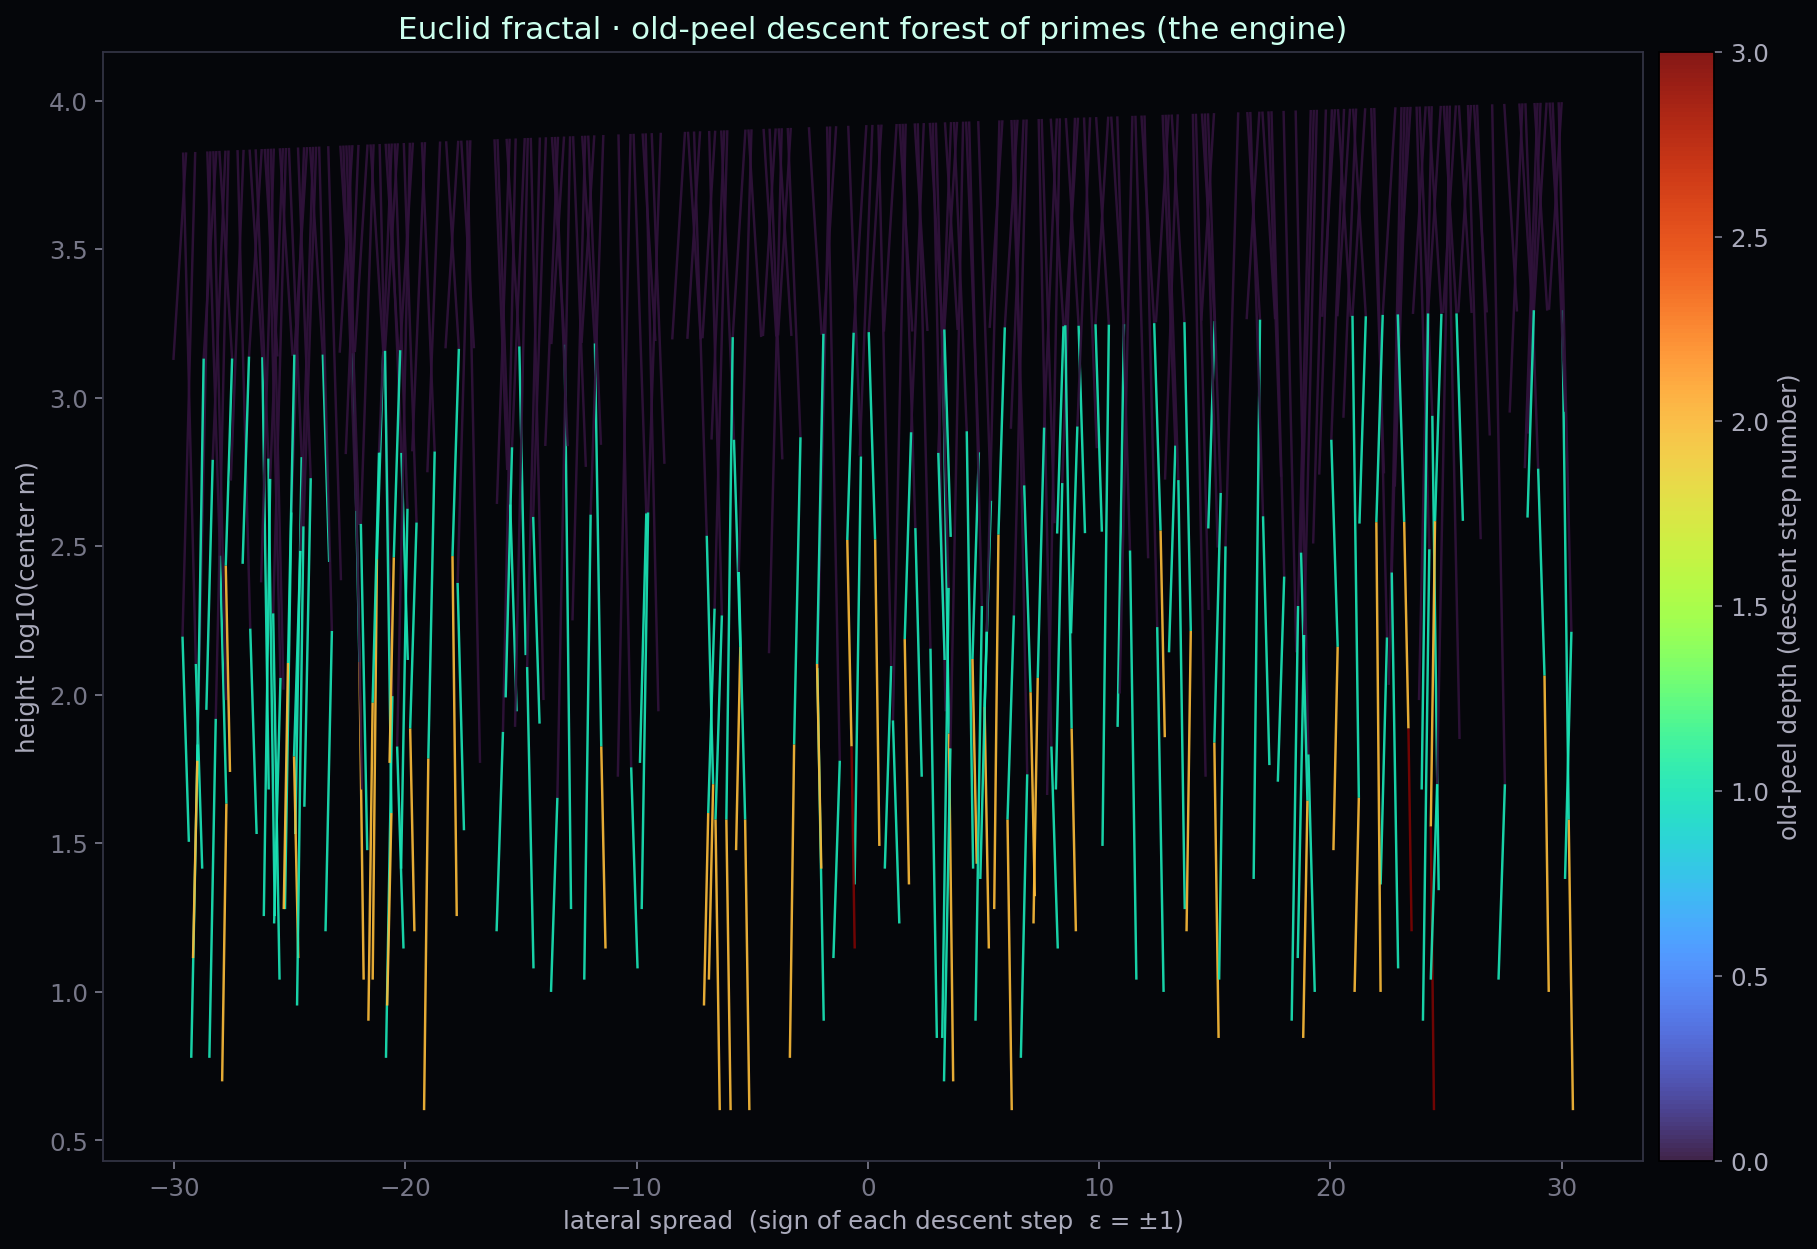
\includegraphics[width=\linewidth]{figures/1_old_peel_tree.png}
  \caption{The old-peel descent forest of primes --- the engine itself, run
  recursively from a row of large centres.}
  \label{fig:old-peel-tree}
\end{figure}

\emph{Generation algorithm (Figure~\ref{fig:old-peel-tree}).} Source:
\srcpath{tools/fractal/euclid\_fractal.py::old\_peel\_tree}. Fix $A=200$ and sieve
all primes up to $4A^2$; let the caught-prime pool be the primes $p$ with
$3<p\le A$. Seed a horizontal row of $460$ roots at abscissae $x$ evenly spaced
over $[-30,30]$, the $i$-th root carrying centre $n=\lfloor A^2/6\rfloor+7i$.
From each root run the recursive descent $\mathrm{peel}(n,\varepsilon,d,x)$ for
both signs $\varepsilon=\pm1$: it stops when depth $d>7$ or $n<2$; it requires
the side $a=6n+\varepsilon$ to be prime with $a>A$; it takes the opposite side
$6n-\varepsilon$, finds the first pool prime $p$ dividing it, forms the quotient
$q=(6n-\varepsilon)/p$, reads its sign $\delta$ from $q\bmod6$ ($\delta=+1$ if
$q\equiv1$, $\delta=-1$ if $q\equiv5$, aborting otherwise), and sets the child
centre $t=(q-\delta)/6$ (aborting if $t\le0$). The step draws a segment from
$(x,\ \log_{10}(n+1))$ to $(x+\varepsilon\cdot0.55/(d+1),\ \log_{10}(t+1))$, then
recurses into $t$ with both signs at depth $d+1$. The vertical axis is height
$\log_{10}(\text{centre})$; the horizontal offset encodes the descent sign
$\varepsilon$; segments are coloured by descent depth $d$ (turbo palette).

\begin{figure}[H]
  \centering
  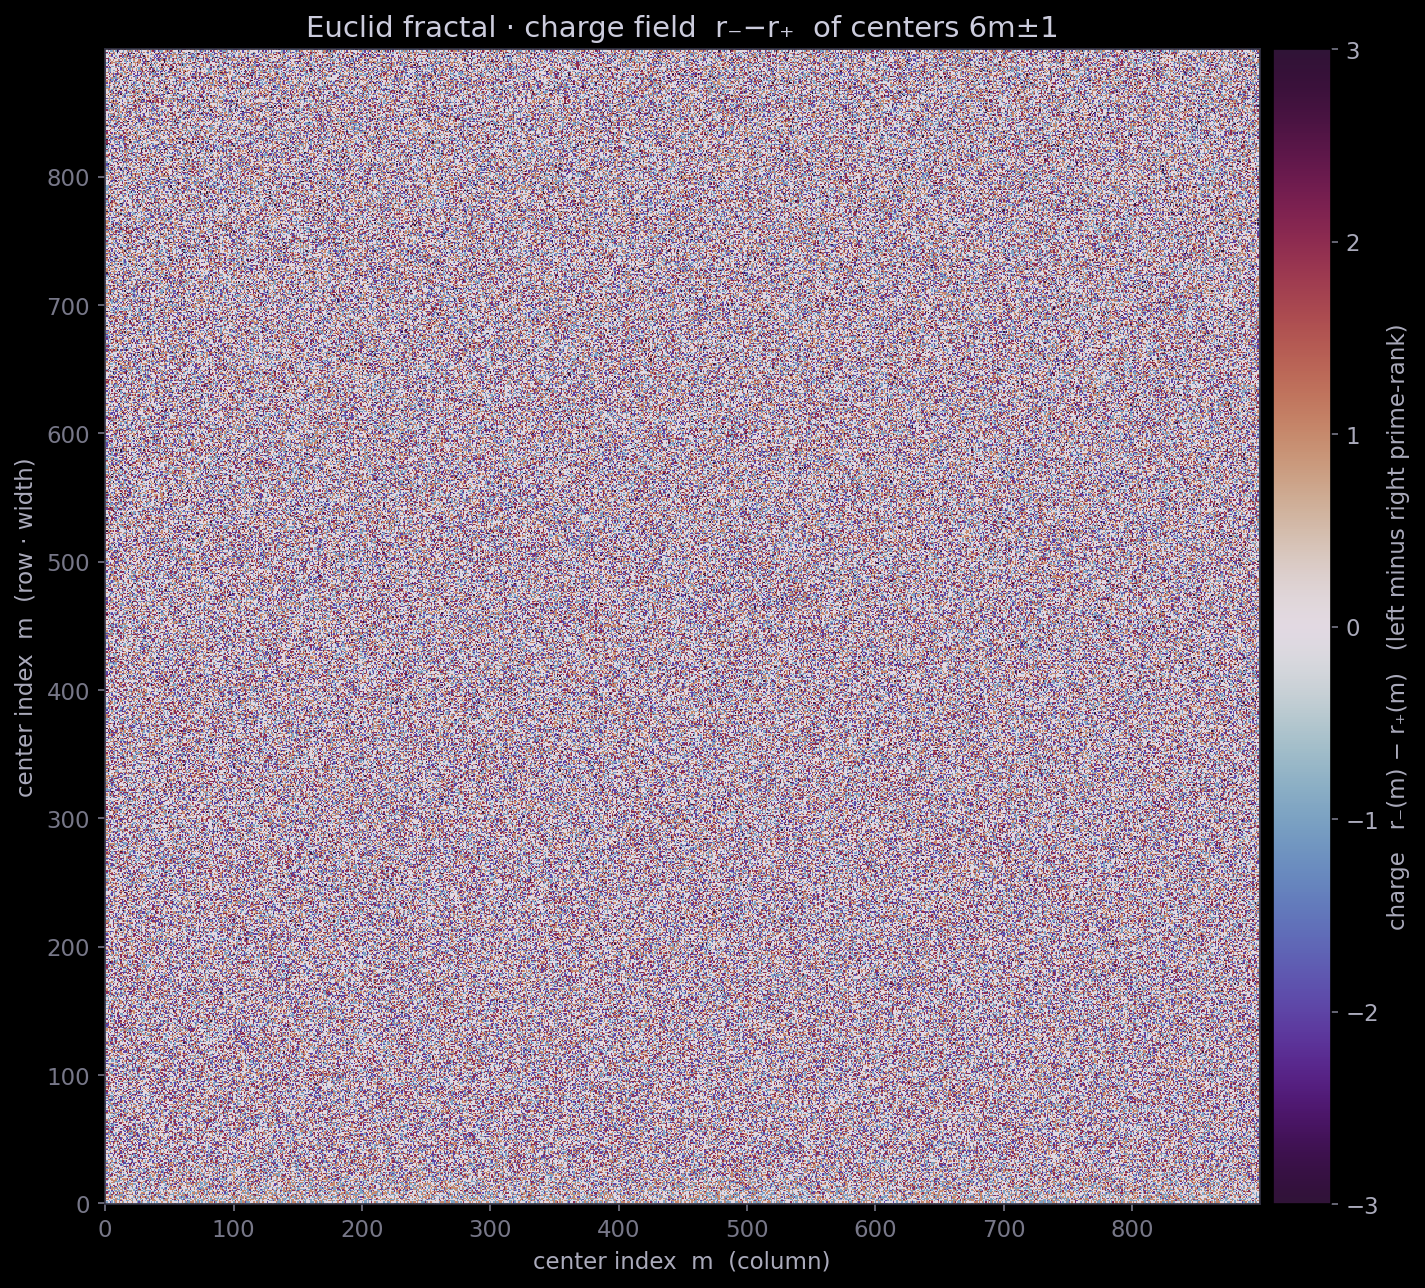
\includegraphics[width=\linewidth]{figures/2_rank_field.png}
  \caption{The charge field $r_-(m)-r_+(m)$ of the centres $6m\pm1$: the
  fractal generating function of prime rank.}
  \label{fig:rank-field}
\end{figure}

\emph{Generation algorithm (Figure~\ref{fig:rank-field}).} Source:
\srcpath{tools/fractal/euclid\_fractal.py::rank\_field}. Parameters $A=60$,
$W=900$; the prime layer is $\{p:\ A<p\le A^2\}$. For each centre index
$m\in\{0,\dots,W^2-1\}$ two ranks are counted: $r_-(m)$, the number of layer
primes dividing the lower side $6m-1$, and $r_+(m)$, the upper side $6m+1$. For
each $p$ the congruence $6m\equiv\pm1\pmod p$ is solved via the inverse
$6^{-1}\bmod p$, giving the root $r\equiv\pm6^{-1}\pmod p$, the start offset
$(r-1)\bmod p$, and a unit added to every $p$-th position of the array $r_\mp$.
The charge $r_-(m)-r_+(m)$ is imaged: the length-$W^2$ vector is reshaped into a
$W\times W$ matrix (row $=\lfloor m/W\rfloor$, column $=m\bmod W$) and drawn with
the diverging twilight-shifted palette (opposite charge signs at the two ends,
zero at the centre), lower origin.

\begin{figure}[H]
  \centering
  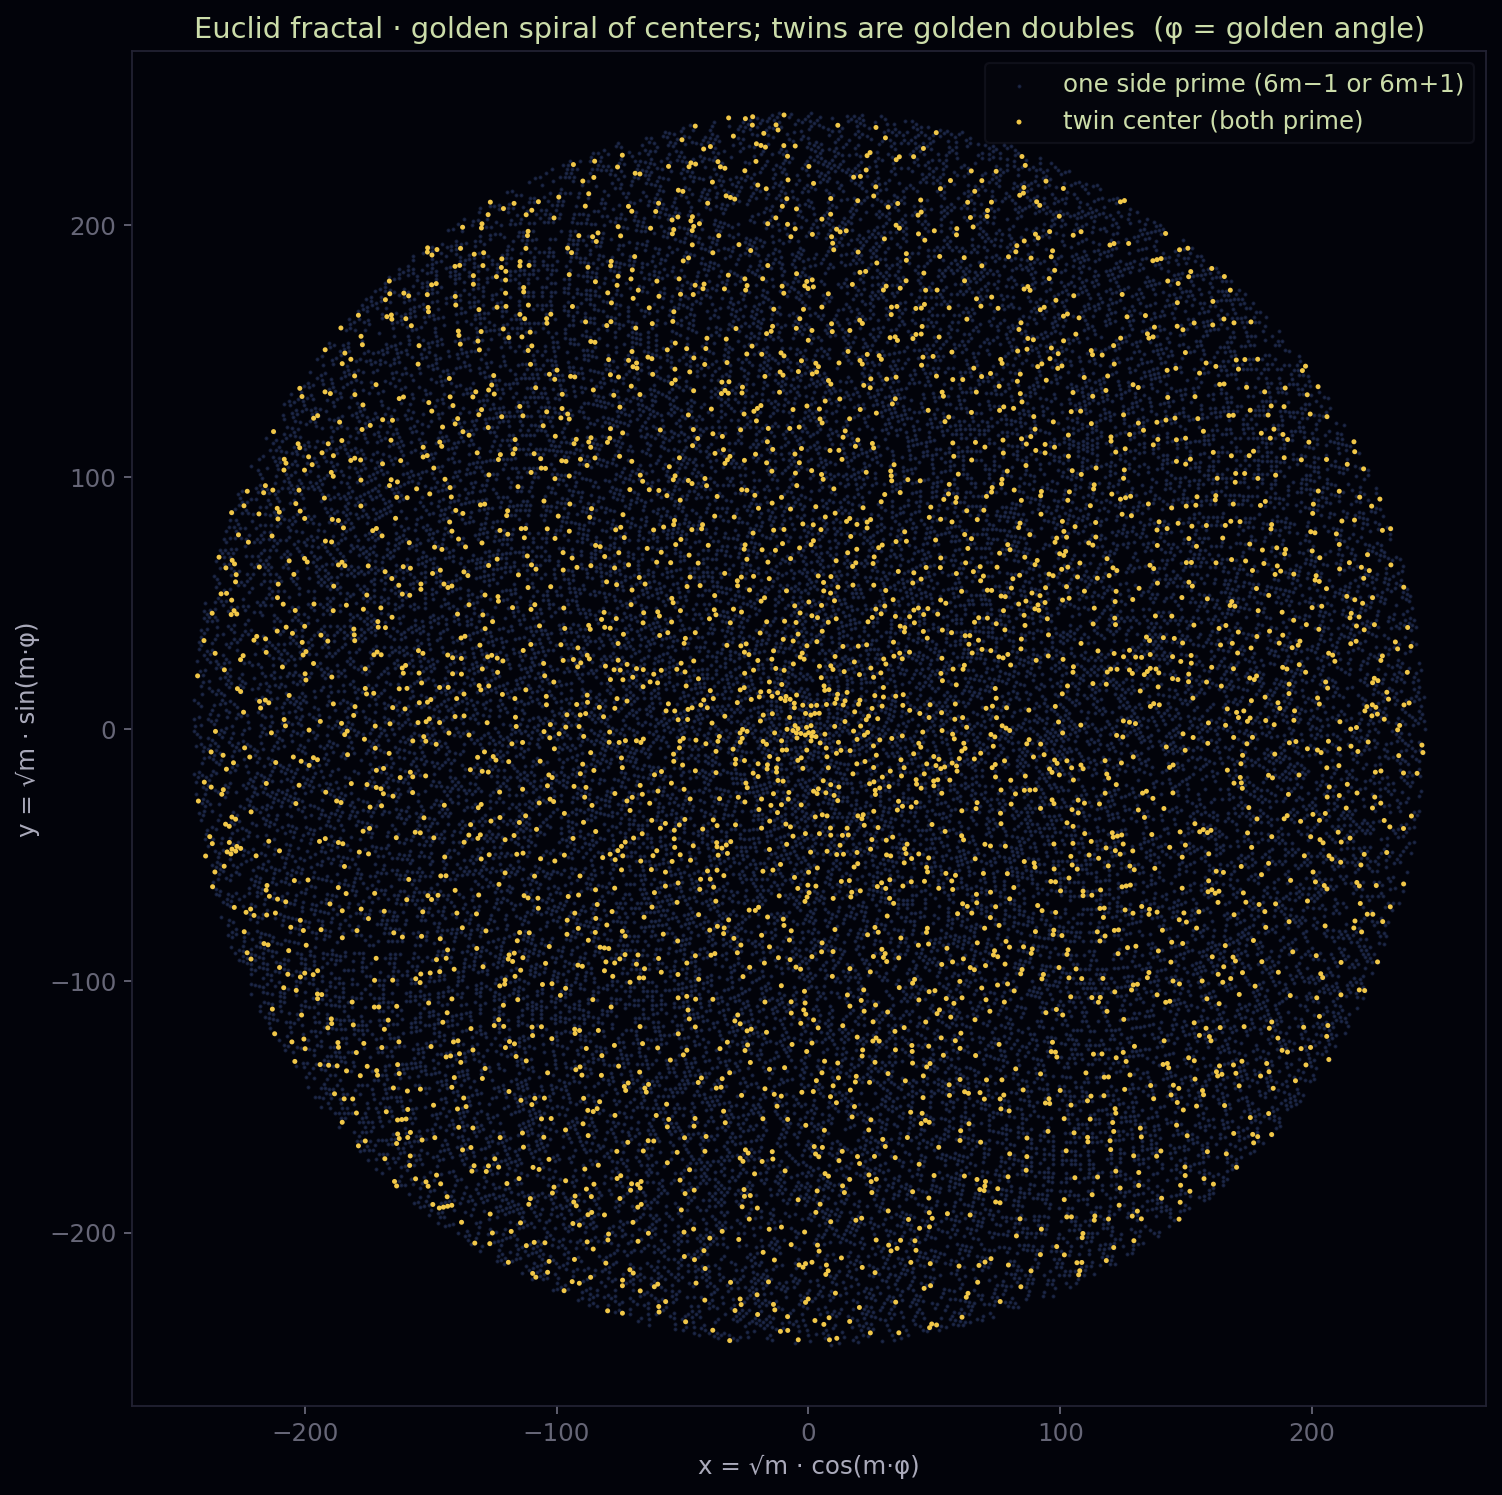
\includegraphics[width=\linewidth]{figures/3_twin_spiral.png}
  \caption{The golden spiral of centres; twin-centres are the golden doubles.}
  \label{fig:twin-spiral}
\end{figure}

\emph{Generation algorithm (Figure~\ref{fig:twin-spiral}).} Source:
\srcpath{tools/fractal/euclid\_fractal.py::twin\_spiral}. For each centre
$m=1,\dots,M-1$ (default $M=60000$) a point is placed on the golden spiral
\begin{equation}\label{eq:golden-spiral}
  x=\sqrt{m}\,\cos(m\varphi),\qquad
  y=\sqrt{m}\,\sin(m\varphi),\qquad
  \varphi=\pi(3-\sqrt5),
\end{equation}
with $\varphi$ the golden angle. A centre is marked one-sided prime when
$6m-1$ or $6m+1$ is prime (dim blue points), and a twin-centre when both sides
$6m\pm1$ are prime (large golden points). The radius $\sqrt m$ gives uniform
density per unit area; the colour is fixed per class.

\begin{figure}[H]
  \centering
  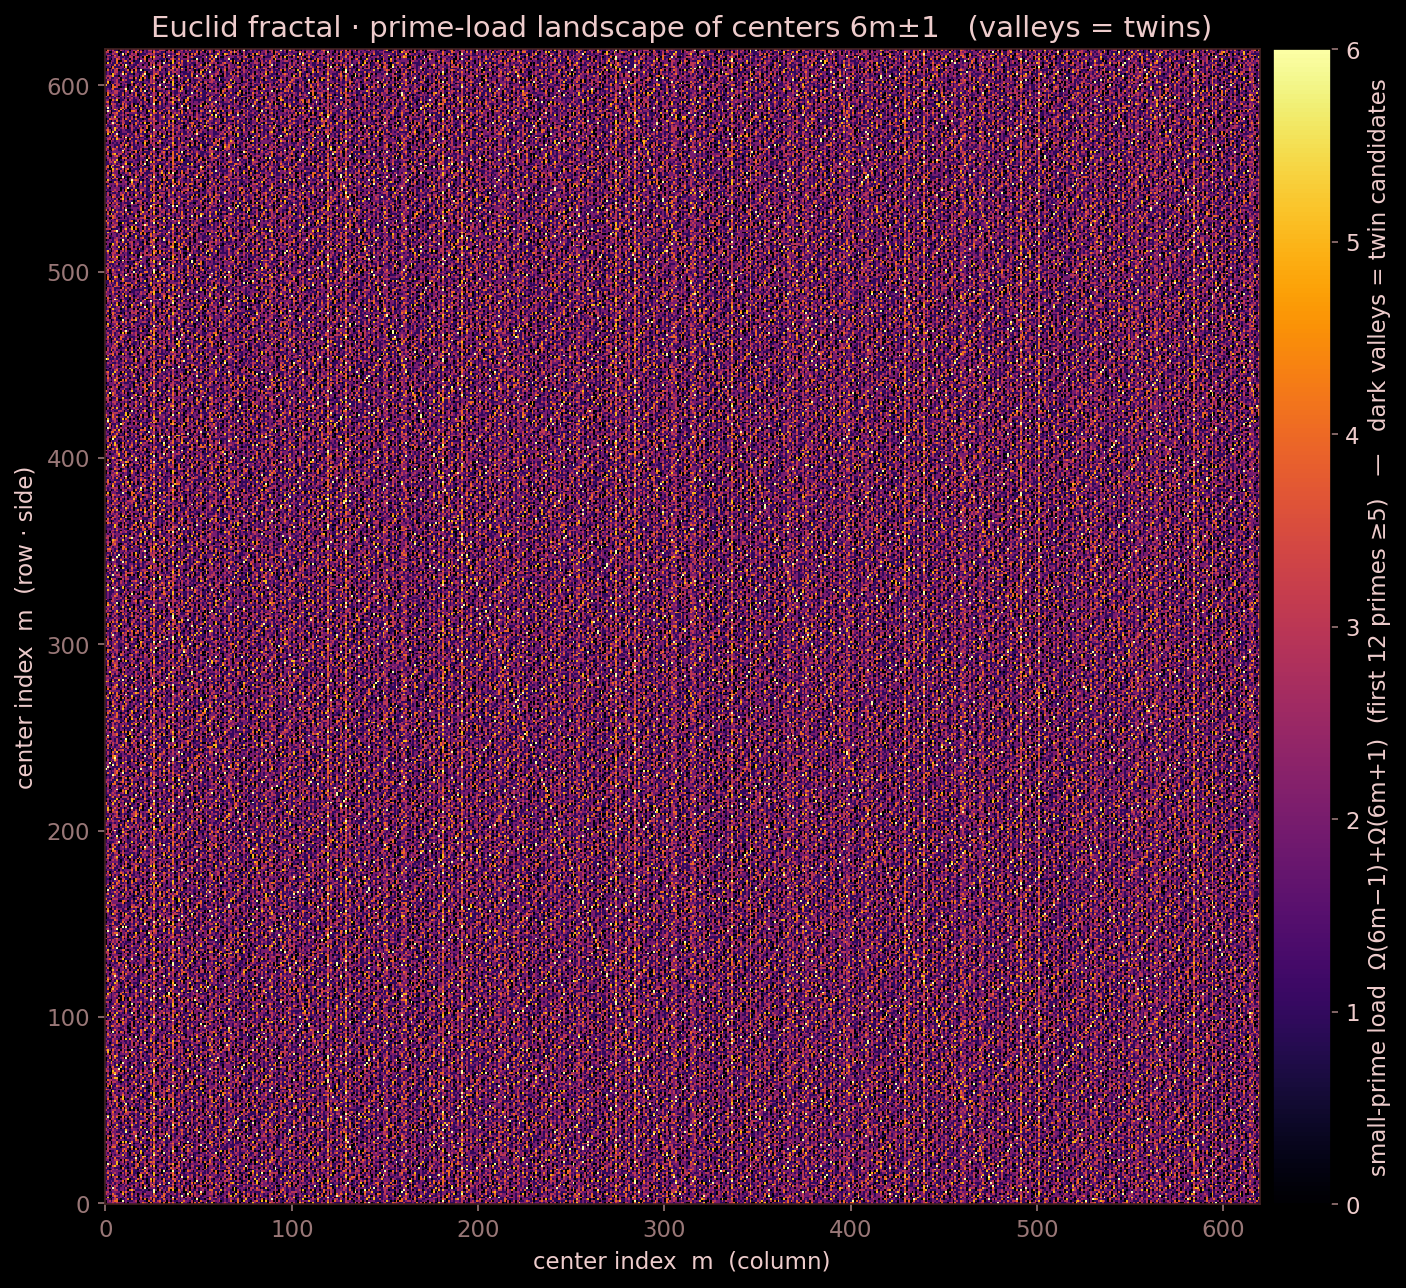
\includegraphics[width=\linewidth]{figures/4_descent_landscape.png}
  \caption{The prime-load landscape of the centres $6m\pm1$; the dark valleys
  are the twin candidates.}
  \label{fig:descent-landscape}
\end{figure}

\emph{Generation algorithm (Figure~\ref{fig:descent-landscape}).} Source:
\srcpath{tools/fractal/euclid\_fractal.py::descent\_landscape}. For every centre
$m=0,1,\dots,S^2-1$ laid on an $S\times S$ raster ($S=620$, row-major in $m$),
compute the small-prime load
\begin{equation}\label{eq:small-prime-load}
  L(m)\;=\;\Omega_B(6m-1)+\Omega_B(6m+1),
\end{equation}
where $\Omega_B(x)$ is the number of prime factors of $x$, counted with
multiplicity and restricted to the first $B=12$ primes $\ge5$ (that is,
$5,7,11,\dots,41$). Colour each cell by $L(m)$ (inferno palette, clipped at the
99th percentile). Twin centres --- where both sides $6m\pm1$ are prime --- have
$L(m)=0$ and appear as the dark valleys; the self-similar relief is the
Chinese-remainder periodicity of the small primes.

\begin{figure}[H]
  \centering
  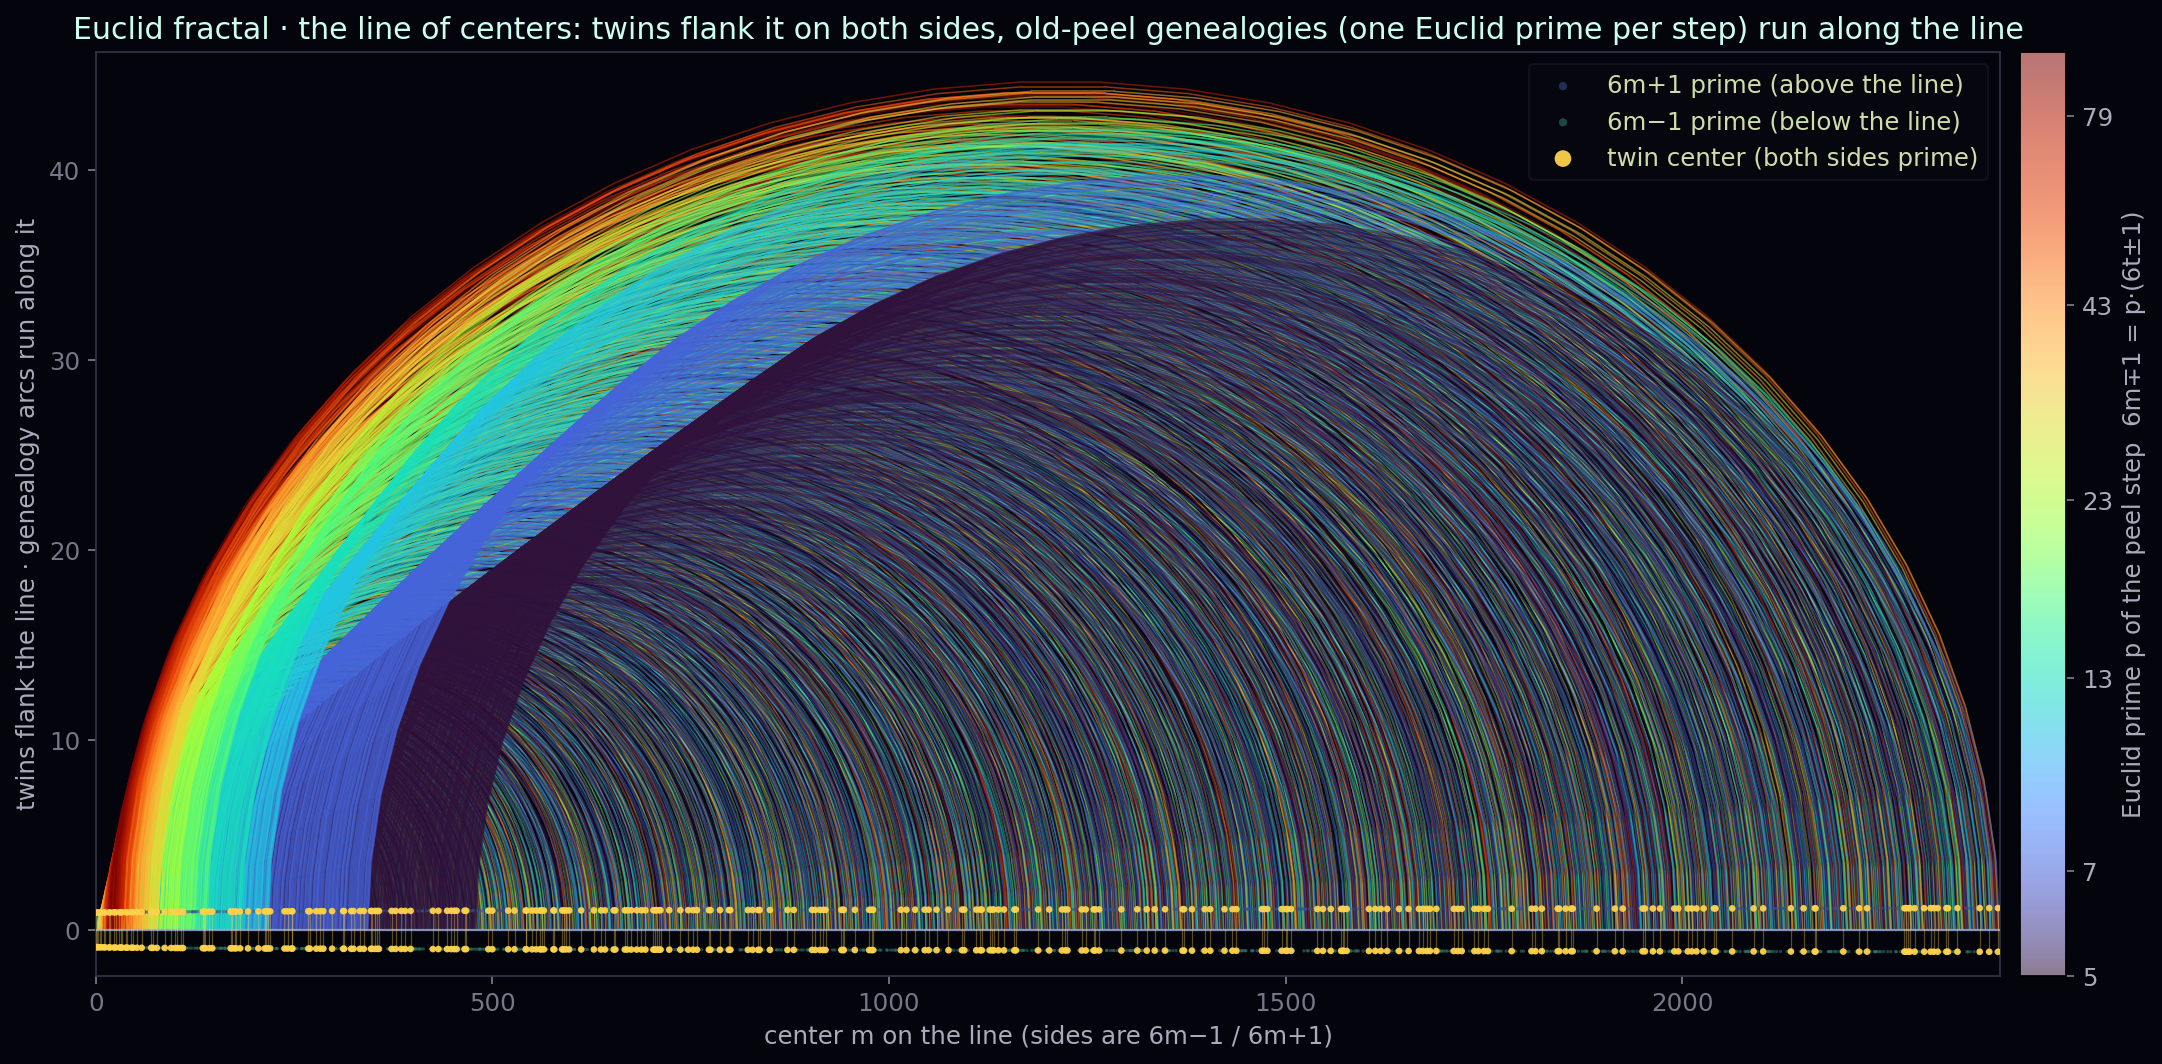
\includegraphics[width=\linewidth]{figures/5_twin_line_genealogy.png}
  \caption{The line of centres: twins flank it on both sides, old-peel
  genealogies (one Euclid prime per step) run along it.}
  \label{fig:twin-line-genealogy}
\end{figure}

\emph{Generation algorithm (Figure~\ref{fig:twin-line-genealogy}).} Source:
\srcpath{tools/fractal/euclid\_fractal.py::twin\_line\_genealogy}. Centres
$m=1,\dots,M$ ($M=2400$) are laid along the horizontal axis $y=0$. The side
$6m+1$ is marked by a point \emph{above} the line at height
$\mathrm{wing}(m)=0.9+0.25\sqrt{m/M}$, the side $6m-1$ by a symmetric point
below, whenever the corresponding number is prime (sieve to $6M+2$). A twin
centre (both sides prime) is marked by a golden vertical
$[-\mathrm{wing},\,+\mathrm{wing}]$ with points at its ends. Along the line, for
each $m$ the old-peel step is computed: if $6m\mp1=p\,(6t\pm1)$ with a Euclid
witness prime $p\in[5,97]$, a semicircular arc $m\to t$ is drawn of height
$h=0.06\,|m-t|^{0.85}+0.4$ (36 points,
$x=\tfrac{m+t}{2}+\tfrac{|m-t|}{2}\cos\theta$, $y=h\sin\theta$,
$\theta\in[0,\pi]$), coloured by $\log p$ (turbo palette). Twin centres live
\emph{off} the line, the genealogy \emph{on} it.

\begin{figure}[H]
  \centering
  \includegraphics[width=\linewidth]{figures/6_genealogy_ornament.png}
  \caption{The genealogy ornament: the full old-peel descent of every centre,
  woven as chords on the circle of centres.}
  \label{fig:genealogy-ornament}
\end{figure}

\emph{Generation algorithm (Figure~\ref{fig:genealogy-ornament}).} Source:
\srcpath{tools/fractal/euclid\_fractal.py::genealogy\_ornament} ($M=4200$,
$\mathrm{PMAX}=97$, $\mathrm{DEPTH}=10$). Centres $1,\dots,M$ sit on the unit
circle at angle $2\pi m/M$. For each centre the full old-peel genealogy
$m\to t_1\to t_2\to\cdots$ (to depth $10$) is built by the step
$6k\mp1=p\,(6t\pm1)$: each step is a Bézier chord with control point
$\tfrac12(P_a+P_b)\cdot(1-0.92\min(2\Delta\theta,1))$, where
$\Delta\theta=|a-b|/M$ (long chords dive deeper toward the centre); colour by
$\log p$ (turbo). Twin-centres (empty genealogy) sit on the rim as golden
points.

The two remaining figures are conceptual: they place the \emph{real}
genealogy in a cosmological picture. We stress the honest boundary, exactly as
in the coda: only the irreversibility of time and the curvature of space are
rigorously proved (the engine impossibility of \cref{sec:engine}); the reading
of the pictures as physics is a translation, not a theorem.

\begin{figure}[H]
  \centering
  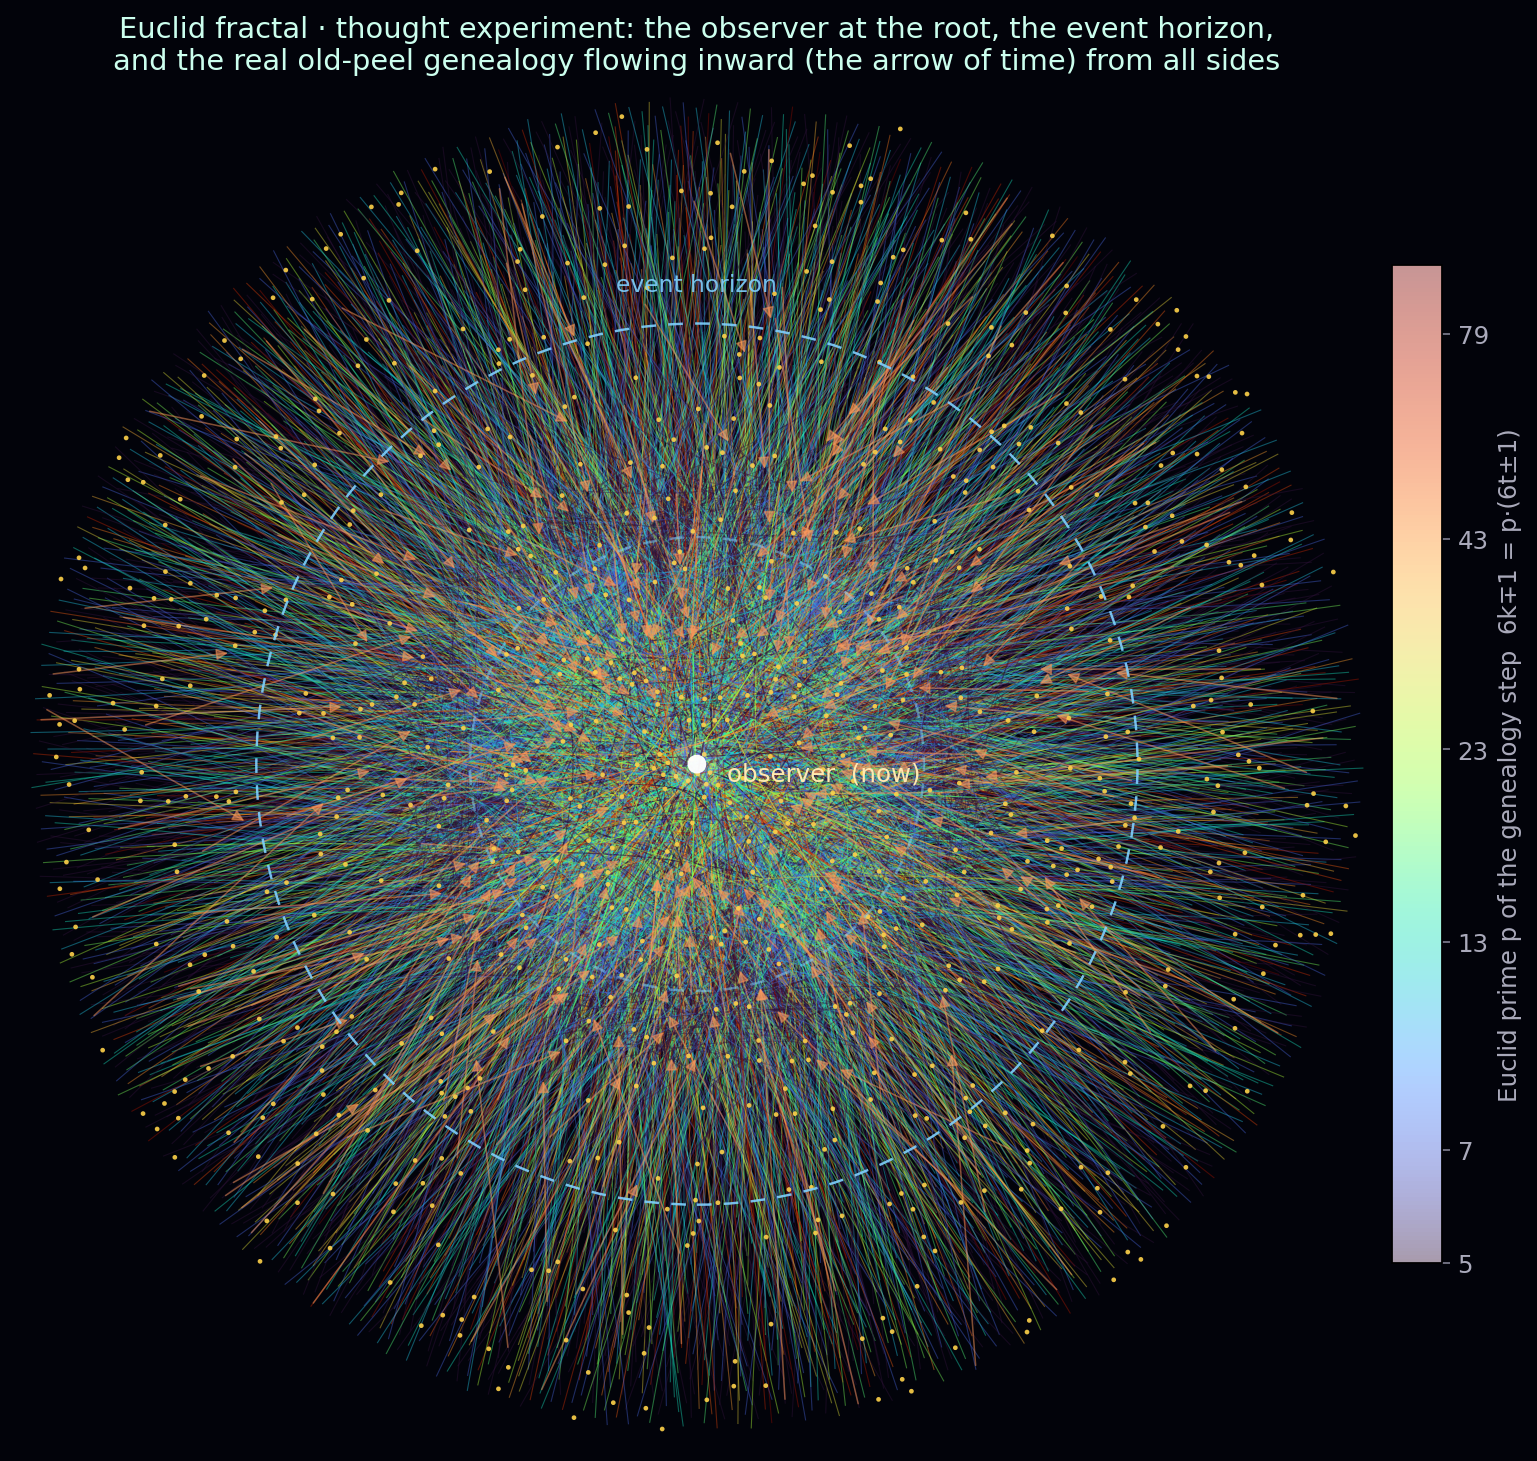
\includegraphics[width=\linewidth]{figures/7_observer_horizon.png}
  \caption{Thought experiment: the observer at the root, the event horizon, and
  the real old-peel genealogy flowing inward (the arrow of time).}
  \label{fig:observer-horizon}
\end{figure}

\emph{Generation algorithm (Figure~\ref{fig:observer-horizon}).} Source:
\srcpath{tools/fractal/euclid\_cosmology.py::observer\_horizon} ($M=9000$,
$\mathrm{PMAX}=97$, $\mathrm{DEPTH}=9$). Centre $k$ is placed on a golden spiral
by radius-height $r=\sqrt{k/M}$ and angle $k\varphi$ ($\varphi$ the golden
angle): small $k$ near the centre (the observer), large $k$ on the periphery.
The full old-peel genealogy of each centre is built by the step
$6k\mp1=p\,(6t\pm1)$ (smallest prime divisor $p\in[5,97]$ of the composite side,
$t<k$), iterated to depth $9$. Each step $k\to t$ is drawn as a quadratic Bézier
with control point $\tfrac12(P_k+P_t)\cdot0.72$ pulled toward the origin (the arc
dives inward); colour by $\log p$ (turbo palette). Orange arrows are placed on
real first steps with $r>0.30$ and point from $k$ to $t$ (inward). The dashed
circles of radius $0.66$ and $0.34$ are the event horizon; golden dots are
twin-centres.

\begin{figure}[H]
  \centering
  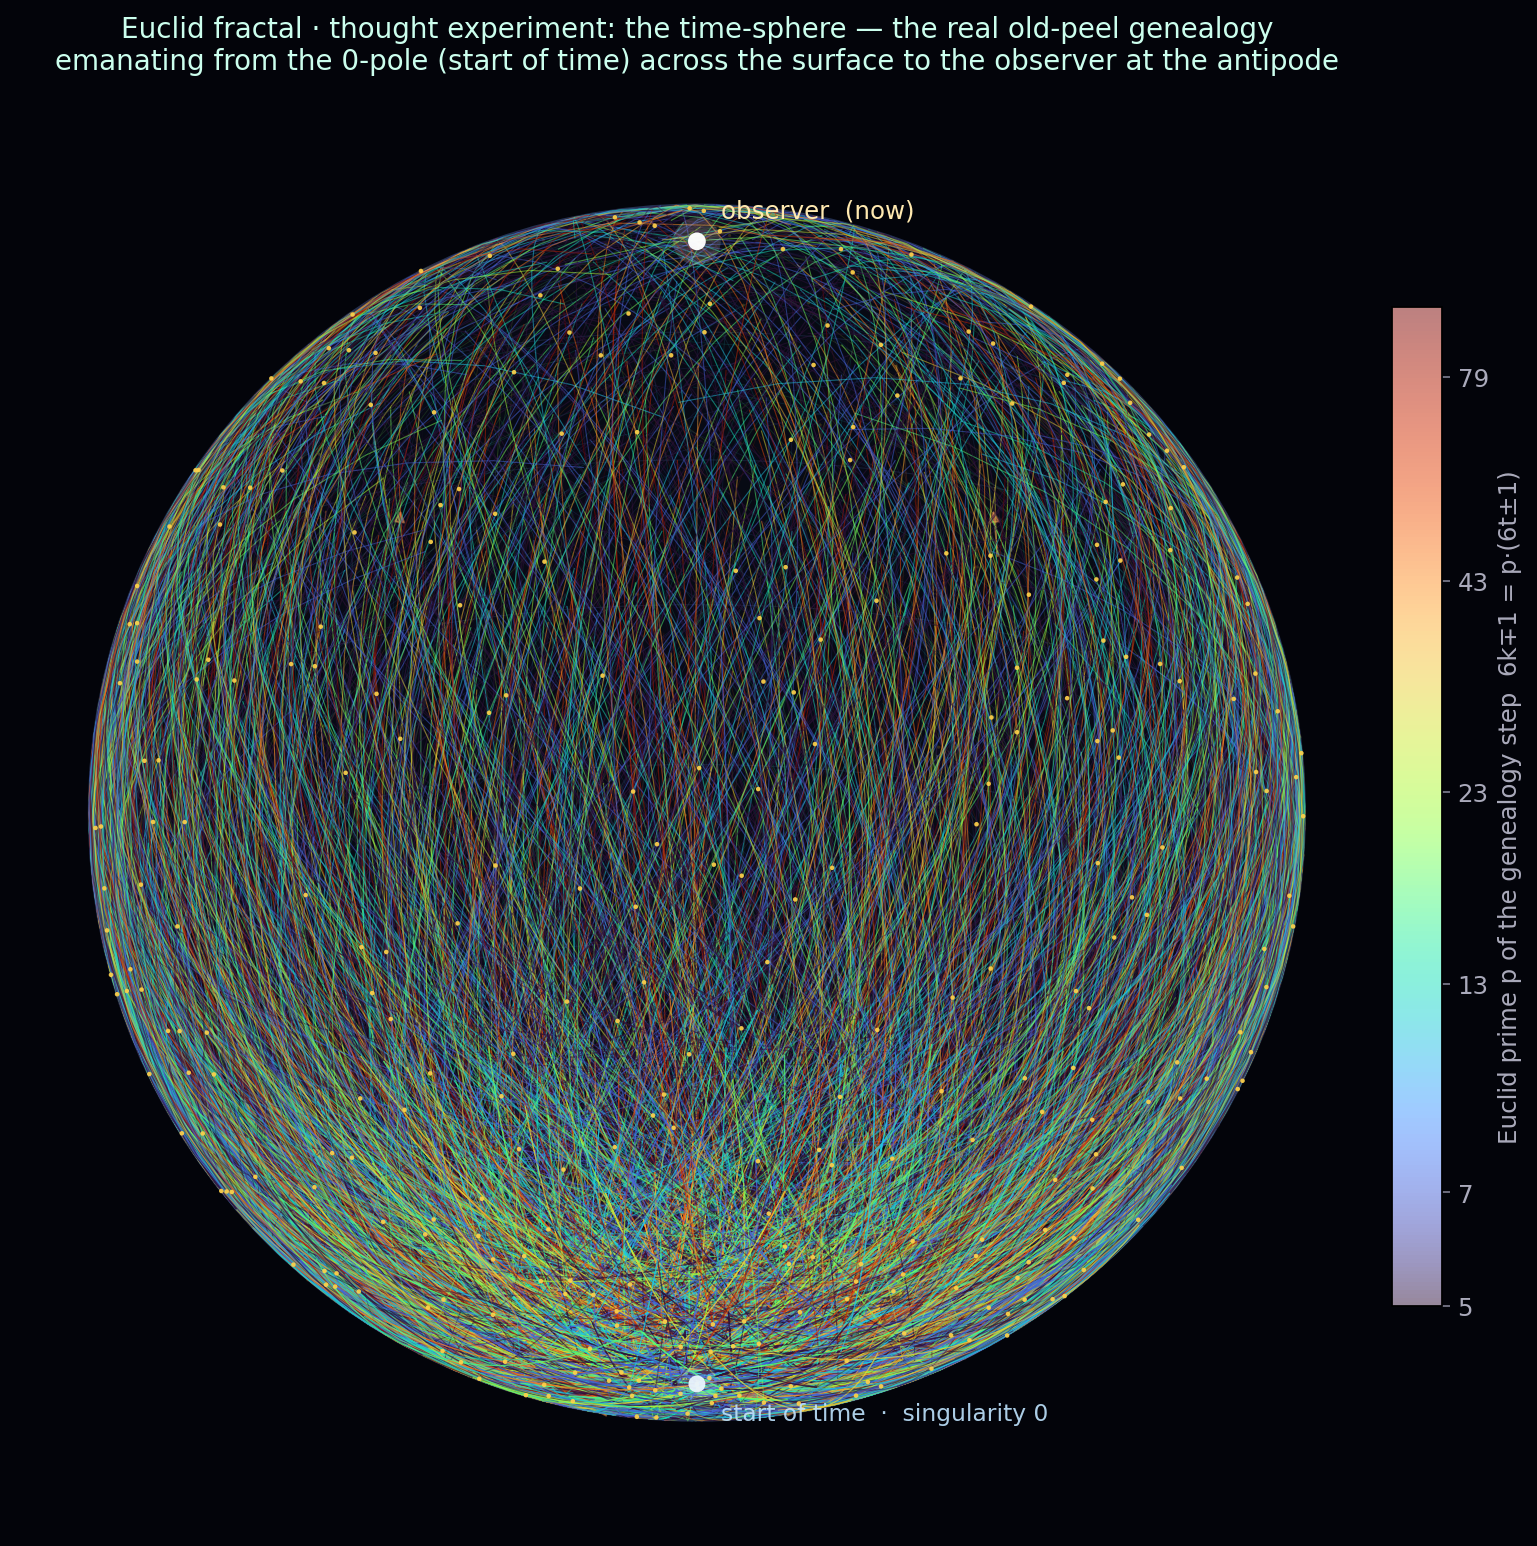
\includegraphics[width=\linewidth]{figures/8_time_sphere.png}
  \caption{Thought experiment: the time-sphere --- the real old-peel genealogy
  emanating from the $0$-pole (start of time) to the observer at the antipode.}
  \label{fig:time-sphere}
\end{figure}

\emph{Generation algorithm (Figure~\ref{fig:time-sphere}).} Source:
\srcpath{tools/fractal/euclid\_cosmology.py::time\_sphere} ($M=7000$,
$\mathrm{PMAX}=97$, $\mathrm{DEPTH}=9$). Centre $k$ maps to a unit vector on the
sphere: height $z=-1+2(k-1)/(M-1)$ (so $k=1$ is at the $0$-pole, $z=-1$; $k=M$ at
the observer-pole, $z=+1$), longitude $k\varphi$ by the golden angle,
$\rho=\sqrt{1-z^2}$. The full old-peel genealogy $6k\mp1=p\,(6t\pm1)$ (depth $9$)
is drawn as great-circle arcs (spherical slerp between $V_k$ and $V_t$);
front-hemisphere arcs bright, back-hemisphere faint; colour by $\log p$ (turbo).
The projection is a $20^\circ$ rotation about the $x$-axis. Orange meridian
arrows mark the generative direction of time from the $0$-pole to the
observer-pole; golden dots are twin-centres; the two poles are labelled
``observer (now)'' and ``start of time $\cdot$ singularity $0$''.


\bibliographystyle{plain}
\bibliography{refs}

\end{document}
